\section[FE Theory for the Helmholtz Equation]{The theory of the $h$-finite-element dis\-cret\-i\-sa\-tion of the Helmholtz equation}\label{sec:helmfe}

We now shift our attention to the numerical analysis of the Helmholtz equation in heterogeneous media; in particular, we  study the conforming finite-element method for the Helmholtz equation. We first state the variational formulations of the Helmholtz equation, define the finite-element method, and recall results on the approximation properties of finite-element spaces. We then prove our main result, error bounds for the finite-element method for the heterogeneous Helmholtz equation, where the bounds hold for arbitrary (fixed) degree finite elements, and are explicit in $A$ and $n$ in a sense made clear in \cref{sec:fem} below.

  \subsection{Variational formulations for the Helmholtz equation}\label{sec:varform}
  The finite-element method is based on the variational formulation of the Helmholtz equation; for simplicity of exposition, we state the variational formulation of \cref{prob:edp,prob:tedp} in the case $\gD = 0,$ although these can be generalised to the case $\gD \neq 0.$
  
\bprob[Variational formulation of EDP when $\gD = 0$]\label{prob:vedp}
Let $\Dp, A, n,$ and $f$ be as in \cref{prob:edp}. Choose $R>0$ such that $\supp f,$ $\supp(I-A),$ $\supp(1-n) \compcont \BR,$ and define $\DR \de \Dp \cap \BR.$

We say $u \in \HozDDR$ satisfies the \defn{variational formulation of the exterior Dirichlet problem} with $\gD = 0$ if
\beqs
\aE(u,v) = \FE(v)\quad \tfa v \in \HozDDR,
\eeqs
where
\beq\label{eq:aedp}
\aE(w,v) \de \int_{\DR} \mleft(\mleft(A \grad w\mright)\cdot\grad \vbar - k^2 n\minispace w \vbar\mright) - \DPGR{\DtN \trGR w}{\trGR v}
\eeq
and
\beq\label{eq:Ledp}
\FE(v) \de \int_{\DR} f\minispace\vbar,
\eeq
where $\DtN:\HhGR\rightarrow \HmhGR$ is the Dirichlet-to-Neumann map for the homogeneous Helmholtz equation $\Lap u + k^2 u = 0$ combined with the Sommerfeld radiation condition in the exterior of $\BR$; and $\DPGR{\cdot}{\cdot}$ is the duality pairing on $\GR.$
\eprob

\ble[Equivalence of formulations for the EDP]\label{lem:edpform}
\Cref{prob:edp,prob:vedp} are equivalent in the following sense. If $u \in \HolocDp$ solves \cref{prob:edp}, then $u\restrict_{\DR} \in \HozDDR$ and $u\restrict_{\DR}$ solves \cref{prob:vedp}  (for $R$ as in \cref{prob:vedp}). Conversely, if $u \in \HozDDR$ solves \cref{prob:vedp}, then $u$ solves \cref{prob:edp}, if $u$ is extended to $\HolocDp$ by the solution of the exterior Dirichlet problem (in the exterior of $\DR$) for the homogeneous Helmholtz equation with the Sommerfeld radiation condition (with Dirichlet data $\tr u$ on $\partial \BR$).
\ele

For a proof of \cref{lem:edpform}, see \cite[Lemma 3.3]{GrPeSp:19}.

\bprob[Variational formulation of TEDP when $\gD = 0$]\label{prob:vtedp}
Let $D, A, n, f,$ and $\gI$ be as in \cref{prob:tedp}. We say $u \in \HozDD$ satisfies the \defn{variational formulation of the truncated exterior Dirichlet problem} with $\gD = 0$ if
\beq\label{eq:vtedp}
\aT(u,v) = \FT(v) \tfa v \in \HozDD,
\eeq
where
\beq\label{eq:aT}
\aT(w,v) \de \int_{D} \big(\mleft(A \grad w\mright)\cdot\grad \vbar - k^2 n\minispace w \vbar\big) - ik\DPGI{\trGI w}{\trGI v}
\eeq
and
\beqs
\FT(v) \de \int_{D} f\minispace\vbar + \DPGI{\gI}{\trGI v}
\eeqs
\eprob

\ble[Equivalence of formulations for the TEDP]\label{lem:tedpform}
\Cref{prob:tedp,prob:vtedp} are equivalent, i.e., $u \in \HozDD$ solves \cref{prob:tedp} if, and only if, $u$ solves \cref{prob:vtedp}.
\ele

For a proof of \cref{lem:tedpform}, see \cite[Lemma A.7]{GrPeSp:19}.
  
\subsection{Background concepts in finite-element theory}\label{sec:fetheory}

We now give a brief summary of elementary concepts in finite-element theory. For brevity, we focus only on those concepts that we need to prove the new error bounds for finite-element discretisations of the Helmholtz equation in \cref{thm:fembound} below. We denote the spatial domain by $D.$

Throughout this thesis, we will assume that our finite-element space is defined on a conforming triangulation of simplices in the sense of Ciarlet \cite[Paragraphs (FEM1) p. 61 and ($\cT_{h}$5) p. 71]{Ci:91} which we now recall.

\bde[Conforming triangulation of simplices]\label{def:triangulation}
We say that $\cT$ is a \defn{conforming triangulation of simplices over $D$} (or simply \defn{triangulation}) if $\Dclos$ is subdivided into a finite number of simplices $T \in \cT$ such that
\ben
\item For each $T \in \cT$, the set $T$ is closed and the interior $\Tint$ is nonempty and connected.
\item For each $T \in \cT,$ the boundary $\partial T$ is Lipschitz.
\item The equality \beqs
\Dclos = \bigcup_{T \in \cT} T
\eeqs
holds.
\item For each $T_1 \neq T_2 \in \cT,$ we have $\Tint_1 \cap \Tint_2 = \emptyset.$
  \item For any $T_1 \in \cT,$ any face of $T_1$ is either a subset of $\dD$ of a face of a different simplex $T_2 \in \cT.$
\een
\ede

We also define the mesh size of a triangulation.

\bde[Mesh size]
The \defn{mesh size} of a triangulation $\cT$ is given by
\beqs
h \de \max_{T \in \cT} \diam T.
\eeqs
We will frequently denote a triangulation with mesh size $h$ by $\Th.$
\ede

Having defined a triangulation, we are in a position to define the finite-element spaces that we will consider throughout this thesis.

\bde[Finite-element space]\label{def:Vhp}
Let $\Th$ be a triangulation of $D,$ and let $p\geq 1$ be an integer. We let $\Vhp$ be the set of continuous piecewise-polynomials of degree $p$ on $\Th$, i.e.
\beqs
\Vhp \de \set{\vh \in \CzD \st \tforall T \in \Th,\,\vh\restrict_{T} \text{ is a polynomial of degree at most }p}.
\eeqs
\ede

\bre[Do $\Th$ and $\Vhp$ exist?]\label{rem:crimes}
Observe that one can only construct a triangulation $\Th$ of $D$ if $D$ is a polyhedron (since $\dD$ must be the union of faces of simplices). However, observe that, in this case, $\Vhp$ is a conforming subspace of $\HoD$, i.e., $\Vhp \subset \HoD.$ (This inclusion is because the gradient of a function in $\Vhp$ is a piecewise-polynomial function on $\Th,$ which is clearly in $\LtDCCd.$)

However, if $D$ is not a polyhedron (for example, if $D$ is Lipschitz, or $D$ is smooth), then one cannot construct a triangulation $\Th,$ and therefore cannot construct $\Vhp.$ The solution to this problem is to modify the elements near to the boundary, using, e.g., isoparametric finite elements. When using isoparametric finite elements, elements near the boundary are mapped to the reference element using finite-element functions of degree $p,$ instead of using affine functions (as for standard finite elements). The result of this higher-order mapping is that one constructs an approximation of $D$, such that the distance from boundary of the approximation to $\dD$ is $\cO\mleft(h^{p+1}\mright)$ (see, e.g., \cite[Section 4.7]{BrSc:08}). One can then construct a finite-element space on this `curved' mesh, although this finite-element pace will still be nonconforming, and so one must analyse the resulting nonconforming error, as in, e.g., \cite[Section 10.4]{BrSc:08}.

However, in this thesis, we do not work with isoparametric finite elements, because:

\bit
\item This would complicate the presentation further, especially in our new results in \cref{sec:errbounds} below.
\item Our main concern in this \lcnamecref{sec:helmfe} is the $h$- and $k$-dependence of the finite-element-error bounds, rather than the dependence on the geometry of the domain.
\item Other literature concerning finite-element-error bounds for the Helmholtz equation does not include all the details for isoparametric finite elements, see, e.g., \cite[Top of p.785]{DuWu:15} and \cite[Top of p.5]{LaSpWu:19a}.
\item Adapting the results we prove to the case of isoparametric finite elements should be straightforward, as detailed in \cite[Section 10.4]{BrSc:08} (although \cite[Section 10.4]{BrSc:08} works with the stationary diffusion equation, rather than the Helmholtz equation).
\item The only properties of $\Vhp$ that we use are the existence of a best approximation (see \cref{lem:scottzhang} below) and the existence of an inverse inequality (see \cref{lem:inverseinequality} below). Since one can prove an analogous best approximation result for isoparametric finite elements (see, e.g., \cite[Theorem 4.7.3]{BrSc:08}), and we expect one can also prove an analogous inverse inequality (c.f. the proof of the standard inverse inequality in \cite[Section 4.5]{BrSc:08} with the definition of isoparametric finite elements in \cite[Section 4.7]{BrSc:08}), we expect that our original results in \cref{sec:errbounds} below will also hold in the case of isoparametric finite elements.
  \eit

  Therefore, throughout this thesis, we make the following \lcnamecref{ass:conforming} on our triangulations and finite-element spaces, for any spatial domain $D$ arising in this thesis.
  \ere

  \bas[Exact triangulation and conforming subspace]\label{ass:conforming}
We work with a family of triangulations $\mleft(\Th\mright)_{h>0}$ and their corresponding finite-element spaces $\mleft(\Vhp\mright)_{h>0}$, where for any $h>0,$ $\Th$ is a triangulation of $D$ (in the sense of \cref{def:triangulation}), and $\Vhp$ as defined in \cref{def:Vhp} is a conforming subspace of $\HoD.$
  \eas



%%% Assumption - exact triangulation, and therefore conforming


%    \bre[Not considering variational crimes]
%    Throughout this thesis we assume that \cref{prob:fevtedp} is a conforming discretisation of \cref{prob:vtedp}, i.e. $\Vhp \subset \HozDD.$ This inclusion is true if $D$ can be triangulated; otherwise, we must modify the definition of \cref{prob:fevtedp} and commit a variational crime by approximating the boundary of $D$ by a polygon, or introducing mesh elements with curved boundaries using interpolated boundary conditions or isoparametric finite elements. See, e.g., \cite[Chapter 10]{BrSc:08} for an overview of the additional errors introduced by variational crimes (although not in the context of the Helmholtz equation). In this thesis we  ignore such variational crimes, and the additional errors they induce; such analysis is standard. Therefore for the remainder of this thesis we assume that \cref{lem:scottzhang} holds, even if we have not triangulated the domain $D$ exactly.
%    \ere


%we use the terms `mesh` and `triangulation' to refer to a conforming triangulation of simplices in the sense of Ciarlet \cite[Paragraphs (FEM1) p. 61 and ($\cT_{h}$5) p. 71]{Ci:91}. Similarly, we use $h$ to denote the diameter of a mesh\footnote{Frequently in this thesis we will consider families of meshes indexed by their mesh size $h$.}, and we use $\Vhp$ to denote the set of continuous piecewise-polynomials of degree $p$ on a mesh with mesh size $h$.
  %%   triangulation of the domain. (Note that in this thesis we use the words `mesh' and `triangulation' interchangably; strictly speaking, the term `triangulation' only makes sense in 2-d, but we ignore this technicality.

  %%   \bde[Triangulation]
  %%   A triangulation of a polygonal domain $D$ is a finite collection of sets $\Ki \subseteq \Dclos$ such that
  %%   \ben
  %% \item $\interior{\Ki} \cap \interior{\Kj} = \emptyset$ for $ i \neq j,$
  %% \item $\bigcup_i \Ki = \Dclos,$ and
  %%   \item Something about triangles that works in 3-D too\opntodo{Find ref - Brezzi/Johnson? Make sure to use simplical meshes.}.
  %%   \een
  %%   \ede\opntodo{Change to definition in Ciarlet, Handbook of numerical analysis}

%% \bde[Mesh Size]
%% Given a mesh $\cT = \set{\Ki}$ on a domain $D$, the \defn{mesh size} of $\cT$ is defined to be
%% \beqs
%% h = \max_{\Ki} \diam{\Ki}.
%% \eeqs
%% \ede

%%     We can now define finite-element spaces associated with a triangulation; we first define the space of polynomials on a set.

%% \bde[Set of polynomials]
%% For $K \subseteq \RRd,$ $\polyp{K}$ is the set of polynomials defined on $K$ with total degree at most $p.$
%% \ede
%%     \bde[Finite element space of degree $p$]\label{def:fespace}
%%     Given a triangulation $\set{\Ki}$ with mesh size $h$ of a domain $D$, the \defn{(continuous) piecewise-polynomial finite-element space of degree $p$} associated with $\set{\Ki}$ is
%%     \beqs
%% \Vhp \de \set{\vh : D \rightarrow \CC \st \vh \in \CzD \tand \vh\restrict_{\Ki} \in \polyp{\Kiclos} \tforall \Ki }.
%%     \eeqs
%%     \ede

Throughout this thesis, we only consider the $h$-finite-element method, i.e., the degree $p$ of the polynomials associated with the space is assumed fixed, and we consider refining $h.$ This is in contrast to the $p$-finite-element method, where $h$ is fixed and $p$ is increased, and the $hp$-finite-element method, where $h$ is decreased and $p$ is increased according to some rule. Throughout this \lcnamecref{sec:fetheory} we use `finite-element method' to refer to the $h$-finite-element method.

\bre[Why not consider the $hp$-finite element method?]
$hp$-finite-element methods for the homogeneous Helmholtz equation were analysed by Melenk and Sauter in \cite{MeSa:10,MeSa:11}, who showed that the $hp$-finite-element method is quasi-optimal if $kh/p$ is sufficiently small, and $p \gtrsim 1 + \log(k)$ (i.e., we take $p$ growing logarithmically with $k$, and a ($p$-dependent) fixed number of points per wavelength). Such methods can be very effective; the error for such methods can converge exponentially with respect to the number of degrees of freedom (see, e.g., \cite[Theorem 4.51]{Sc:98}). However, their analysis relies on a fully $p$-explicit analysis of the best approximation error of the Helmholtz equation in $hp$-finite-element spaces; such analysis is currently not available for the heterogeneous problem.
\ere

%\ednote{I couldn't immediately see in these results that one obtains exponential convergence with respect to the number of DOFs---have I missed something, or is this result contained somewhere else?}, where they showed one can obtain an exponential rate of convergence with respect to the number of degrees of freedom.
%\opntodo{Get Schwab's hp book and look this up}

%    We adopt the terminology that $\vhptilde$ is the \defn{quasi-interpolant} of $v.$ For a proof of \cref{lem:scottzhang} see, e.g., \cite[Corollary 4.4.24, Remark 4.4.27]{BrSc:08}.

%%     \bre[The function $\vhptilde$]
%% The function $\vhptilde$ in \cref{lem:scottzhang} can be constructed using `averaged Taylor polynomials', see, e.g., \cite{ScZh:90},\cite[Section 4.4]{BrSc:08} for details\footnote{Observe that in \cite{BrSc:08}, the authors use different notation to us; they use $m$ to denote the regularity of $v$ and $p$ to denote the integrability of $v,$ i.e., in \cite{BrSc:08}, $v \in \WmpD.$}.
%%     \ere

    With the concept of a finite-element space established, we can now define the finite-element approximation to the variational problems \cref{prob:vedp,prob:vtedp}.

    \bprob[Finite-element approximation of \cref{prob:vtedp}]\label{prob:fevtedp}
    Find $\uh \in \Vhp$ such that
    \beq\label{eq:fevtedp}
    \aT(\uh,\vh) = \LT(\vh) \tforall \vh \in \Vhp.
    \eeq
    \eprob

    We say that $\uh$ is the \defn{finite-element approximation of $u$} (the solution to \cref{prob:vtedp}). The finite-element approximation of \cref{prob:vedp} is defined analagously.
    
    To state an approximation bound for $\Vhp,$ we first need to define the notion of a shape-regular mesh.

    \bde[Shape-regular]
    For $h>0$ and $\tau \in \Th,$ let $\Btau$ be the largest ball contained in $\tau.$ The mesh family $\mleft(\Th\mright)_{h>0}$ is \defn{shape-regular} if there exists $\rho > 0$ such that for all $h>0$ and for all $\tau \in \Th$
    \beqs
\diam \Btau \geq \rho \diam \tau.
    \eeqs
    \ede

    The following \lcnamecref{lem:scottzhang} shows how the approximation properties of the space $\Vhp$ depend on $h$ and $p$:
    \ble[Existence of approximation]\label{lem:scottzhang}
    Let the mesh family $\mleft(\Th\mright)_{h>0}$ underlying $\mleft(\Vhp\mright)_{h>0}$ be shape-regular. Let $v \in \HmD$, $m \geq 1,$ and $p \in \set{1,\ldots,m}$. Then there exists a constant $\CSZm>0$ independent of $v$ and $\vhptilde \in \Vhp$ such that

    \beqs
\NLtD{v - \vhptilde} \leq \CSZm h^s \NHsD{v}
    \eeqs
     and
    \beqs
\NHoD{v - \vhptilde} \leq \CSZm h^{s-1} \NHsD{v}
\eeqs
for $1 \leq s \leq \min\set{p+1,m}.$
    \ele

    For a proof of \cref{lem:scottzhang} see, e.g., \cite[Theorems 4.4.4 and 4.4.20 and Remark 4.4.27]{BrSc:08}.

    
    

%%     \subsection{Error bound for the heterogeneous IIP}\label{sec:errbound}

%%     We now move on to present new work---bounds on the error $\uh-u$ between the finite-element approximation and the true solution of \cref{prob:vtedp}. These bounds, proven here for the Helmholtz equation in \emph{heterogeneous} media are generalisations of results already in the literature that the finite-element error in the $L^2$- and $H^1$-norms is bounded (as $k\rightarrow \infty$) provided $h \lesssim k^{-(2p+1)/2p}$. These results are crucial for our analysis of the multi-level Monte Carlo method for the Helmholtz equation in \cref{chap:mlmc}.

%% The proof of these results uses a so-called `elliptic projection' technique, introduced by Feng and Wu in \cite{FeWu:09} for Discontinuous Galerkin methods for the Helmholtz equation and modified by Du and Wu \cite{DuWu:15}, where the variational formulation of a PDE related to \cref{prob:vtedp} is used as part of the proof. We  only prove results for \cref{prob:fevtedp}, and not for the finite-element approximation of \cref{prob:vedp}, as our proof uses properties of the related PDE and these properties have only been proven with impedance boundary conditions (in the recent preprint \cite{ChNiTo:18}) and not with an exact Dirichlet-to-Neumann map on the truncation boundary. However, we imagine the results proven for the related PDE with an impedance boundary condition also hold for an exact Dirichlet-to-Neumann boundary condition, and so we anticipate that the results we prove here also hold for finite-element approximations of \cref{prob:vedp}.\opntodo{This paragraph needs rewriting---acknowledge Du \& Wu}

\subsection{Discussion of the finite-element method for the Helmholtz equation}\label{sec:helmfedisc}

We now discuss three possible properties of the $h$-finite-element method for the Helmholtz equation that we wish to investigate:
\bit
\item The relative error $\displaystyle \frac{\NHokD{u-\uh}}{\NHokD{u}}$ is bounded,
\item The error $\NHokD{u-\uh}$ is bounded in terms of norms of the data $f$ and $\gI$, and
  \item The finite-element method is quasi-optimal, $\displaystyle \NHokD{u-\uh} \lesssim \inf_{\vh \in \Vhp} \NHokD{u-\vh},$
    \eit
    with a hidden constant independent of $k$ and $h.$

    The key question we ask is: What mesh conditions lead to each of the three properties above? (I.e., how must one refine $h$ as $k$ increases in order for the finite-element method to satisfy each of the three properties above?)

    We will now summarise the state of the literature regarding each of the three properties above. We will:
    \ben
  \item Define each of the three properties formally,
  \item\label{it:sum2} State the sharpest results known in the literature,
  \item\label{it:sum3} Give a complete overview of all results in the literature concerning the three properties, and
    \item\label{it:sum4} Give a detailed discussion of proof techniques for each of the three properties.
      \een

Regarding \cref{it:sum2,it:sum3}: there is not a complete overview of all of these three properties anywhere in the literature. Moreover, research interest in these three properties has recently increased (e.g., the recent papers \cite{ChNi:18,ChGaNiTo:18,ChNi:19,LiWu:19} are all concerned with one or more of these properties, and have all been completed within the last two years), and so we believe it will be helpful and timely to provide a complete overview of the state of the literature. Regarding \cref{it:sum4}: although the different proof techniques are related, we do not know of anywhere in the literature where these techniques are expounded, compared, and contrasted. We therefore hope that such a review will be valuable for the research community.

      

\paragraph{Intuition for fixed number of points per wavelength}\label{page:ppw} Before discussing the three properties listed above, we first give a brief discussion of the commonly-used heuristic `take a fixed number of points (or elements) per wavelength'.  Recall from \cref{sec:numsolve} that if one takes the mesh size in the finite element method $h \sim 1/k$, then one expects that the interpolation (or best approximation) error is bounded uniformly in $k$. More rigorously, as solutions of the Helmholtz equation typically\footnote{If $f$ and $\gD$ are independent of $k$, and $D$ is smooth enough, or a convex polygon, combining \cref{thm:edp} and standard elliptic regularity results, gives the fact that $\NHtD{u} \lesssim k$, see, e.g., \cite[Lemma 2.12]{GaGrSp:15}.} have $\NHtD{u} \sim k,$ one can bound the $H^1$-norm of the interpolation error independently of $k$ if $h \sim 1/k$ using \cref{lem:scottzhang}:
\beqs
\NHoD{u-\uhptilde} \lesssim h \NHtD{u} \lesssim hk \sim 1.
\eeqs  As explained in \cref{sec:numsolve}, this restriction ensures there are a fixed number of discretisation points per wavelength of the solution, since the wavelength $\lambda = 2\pi/k.$

An alternative motivation for taking $h \sim 1/k$ is the Nyquist--Shannon sampling theorem (proved by Shannon in his seminal paper in information theory \cite[Theorem 1]{Sh:49}). The theorem states that any function $v$ (in 1-d) whose Fourier transform lies inside $[-k,k]$, for some $k>0$, is completely determined (via its Fourier series) by the point values $v(0)$, $v(\pm \mu),$ $v(\pm2\mu),  \ldots$, for any $\mu < 1/\mleft(2k\mright).$ Observe that $k$ is then the highest frequency present in $v$.  That is, if we interpolate $v$ at points spaced less than $ \lambda/(4\pi)=1/(2k)$ apart, where $\lambda = 2\pi/k$ is the wavelength associated with oscillations of frequency $k$, we can reconstruct $v$ from its Fourier transform. See, e.g., \cite[\S 5.21]{BaNaBe:00} for an explicit formula for reconstructioning $v$. Therefore, in the 1-d case we may reasonably expect that interpolating $v$ with points spaced less than $\lambda/(4\pi)$ apart will be a good approximation of $v$, as the Nyquist--Shannon theorem suggests such a spacing of points `captures' all of the oscillations in $v.$
%% The solution of the one-dimensional Helmholtz equation with constant coefficients is
%% \beq\label{eq:hh-1d}
%% u(x) = A \sin(kx) + B \cos(kx),
%% \eeq
%% (for some constants $A$ and $B$), and $\lambda = k/2\pi$ as $u$ has Fourier Transform
%% \beqs
%% \uhat(\xi) = \frac{A}{2i} \mleft(\delta\mleft(\xi-\frac{k}{2\pi}\mright) - \delta\mleft(\xi+\frac{k}{2\pi}\mright)\mright) + \frac{B}{2} \mleft(\delta\mleft(\xi-\frac{k}{2\pi}\mright) + \delta\mleft(\xi+\frac{k}{2\pi}\mright)\mright).
%% \eeqs
%% \opntodo{Find reference}
%% Therefore, if $u$ is sampled at regularly-spaced points that are strictly closer together than $\pi/k = 1/(2\lambda)$, then $u$ can be reconstructed perfectly from these samples.\opntodo{Consider writing something about mutliple dimensions} In conclusion, one expects the be able to interpolate the solution of the Helmholtz equation with uniform error in $k$ if $h \sim 1/k.$

%% However, as was stated in \cref{sec:numsolve}, the finite-element method for the Helmholtz equation suffers from pollution; and $h \sim 1/k$ is not sufficient to keep the finite-element error bounded as $k\rightarrow \infty.$ Therefore we  now provide an overview of previous work giving mesh conditions under which the finite-element error $\NW{u-\uh}$ is bounded as $k\rightarrow \infty$, as well as mesh conditions under which the finite-element method is quasi-optimal. Concerning errors, it would be more natural to consider the relative error $\NW{u-\uh}/\NW{u};$ and to investigate the conditions on $h$ which enable the relative error to be bounded as $k\rightarrow \infty.$ However, current technology typically only allows us to prove results for the error, not the relative error, and so we investigate the error instead.

%We will now briefly review the literature that seeks to answer the question `What mesh condition will keep the relative error bounded as $k \rightarrow \infty$?'


%% \bde[Bounded finite-element error]
%% Let $(\Th)_{h \in (0,1)}$ be a shape-regular family of triangulations of $\DR$, where we assume $h$ is a function of $k$ (e.g., $h(k) = 1/k$). We say that \defn{the error in the finite-element method is bounded uniformly in $k$} if for all $A,n$ in some class there exists $C(A,n)$ (but independent of $k$ and $h$) such that
%% \beqs
%% \NW{u-\uh} \leq C\mleft(\NLtD{f} + \NLtGD{\gD} + \NLtGI{\gI}\mright).
%% \eeqs
%% \ede



 %% In $d=2$ or $3$ with $D$ a convex polygon or polyhedron,  \cite[Theorem 6.1]{Wu:14} showed that the error (but not the relative error) in both the $H^1$ seminorm and the $L^2$ norm is bounded uniformly in $k$ if $h \lesssim k^{-3/2}$. The proof of \cite[Theorem 6.1]{Wu:14} showed an analagous result for a continuous interior-penalty method, and then took the limit as the penalty parameter tends to 0 to obtain the result for the continuous piecewise-linear finite-element method. In summary, the mesh condition $h \lesssim k^{-3/2}$ seems to be sufficient for the (relative) error to be bounded uniformly in $k.$

\subsubsection{Formal definition of the properties of the finite-element method above}\label{sec:femprops}

These definitions may seem overly technical, however their technical definition is necessary to capture the, at times, complicated behaviour of finite-element methods for the Helmholtz equation. Whilst stating the definitions, we give some examples of what they mean for finite-element discretisations of the Helmholtz equation. These definitions are based on, and developed from, \cite[Definition 2.3]{DiMoSp:19}. We define all of these properties for \cref{prob:vtedp} only, although one could define them completely analogously for \cref{prob:vedp}.

In the following definitions, we consider the \cref{prob:vtedp}, and its discretisation \cref{prob:fevtedp}, as parameterised by the wavenumber $k,$ that is, we write $u(k)$ for the solution of \cref{prob:vtedp} with wavenumber $k$, and $\uh(k)$ for its finite-element approximation, the solution of \cref{prob:fevtedp}.

\bde[$\hka{a}$-quasi-optimal]\label{def:hkqo}
Given $a > 0,$ we say that an $h$-finite-element method for the Helmholtz equation is \defn{$\hka{a}$-quasi-optimal} if, given $\kz > 0$, there exist $\Co(\kz), \Cqo(\kz) > 0$ such that if
\beqs
hk^{a} \leq \Co,
\eeqs
then the Galerkin solutions $\uh(k)$ exist, are unique (for each $k$), and satisfy
\beqs
\NHokD{u(k) - \uh(k)} \leq \Cqo \inf_{\vh \in \Vhp} \NHokD{u(k) - \vh},
\eeqs
for all $k \geq \kz.$
\ede

\bde[$\hk{a}{b}$-data-accurate]\label{def:hkdataacc}
Given $a,b>0$, we say that an $h$-finite-element method for \cref{prob:vtedp} is \defn{$\hk{a}{b}$-data-accurate} if, given $0 < \eps < 1,$ and $\kz > 0,$ there exist $\Co(\kz),$ $\Ct(\eps,\kz) > 0$ such that if
\beq\label{eq:hkdataacca}
hk^a \leq \Co
\eeq
and
\beq\label{eq:hkdataaccb}
hk^b \leq \Ct,
\eeq
then the Galerkin solutions $\uh(k)$ exist, are unique (for each $k$), and satisfy
\beq\label{eq:hkdataacc}
\frac{\NHokD{u(k)-\uh(k)}}{\NLtD{f} + \NHhGI{\gI}} \leq \eps \quad \tor \quad \frac{\NHokD{u(k)-\uh(k)}}{\NLtD{f} + \NLtGI{\gI}} \leq \eps
\eeq
for all $k \geq \kz.$

If $a=b$ we say the $h$-finite-element method is $\hka{a}$-data-accurate.
\ede

To aid understanding of the above definition, we give the following illustrative example.

\bre[Example achieving $\hk{a}{b}$-data-accuracy]\label{rem:dataacc}
In \cite[Corollary 4.2]{ZhWu:13}, Zhu and Wu proved that if $u$ is the solution of \cref{prob:vtedp}, $\uh$ is the solution of \cref{prob:fevtedp}, $k \geq \kz$, and $h^{p+1}k^{p+2} \leq \Co$,  then
\beq\label{eq:hkacceg}
\NHokD{u(k) - \uh(k)} \leq \Cttilde \mleft(h + h^pk^p + h^{2p}k^{2p+1}\mright)\mleft(\NLtD{f}+\NHhGI{\gI}\mright)
\eeq
for some $\kz, \Co, \Cttilde > 0.$

For $0 < \eps < 1,$ if we take
\beq\label{eq:egmin}
\Ct = \min\set{\frac{\eps}{3\Cttilde}\kz^{\frac{2p+1}{2p}},\mleft(\frac{\eps}{3\Cttilde}\kz^{\half}\mright)^{\frac1p},\mleft(\frac{\eps}{3\Cttilde}\mright)^{\frac1{2p}}}
\eeq
then the $h$-finite-element method is $\hk{(p+2)/(p+1)}{(2p+1)/(2p)}$-accurate.

When $hk^{(2p+1)/2p} \leq \Ct,$ the first term in the minimum \cref{eq:egmin} ensures $h \leq \eps/\mleft(3\Cttilde\mright),$ the second term in \cref{eq:egmin} ensures $h^pk^p \leq \eps/\mleft(3\Cttilde\mright),$ and the third term in \cref{eq:egmin} ensures $h^{2p}k^{2p+1} \leq \eps/\mleft(3\Cttilde\mright).$ Therefore by \cref{eq:hkacceg} the bound \cref{eq:hkdataacc} holds.

We choose this example to illustrate:
\bit
\item Many results in the literature have $a \neq b$; here $a > b.$
\item Often (as in this case) $a > b.$ I.e., whilst the mesh constraint `$hk^b$ sufficiently small' makes the finite-element error small, the additional constraint `$hk^a$ sufficiently small' is \emph{more} restrictive.
\eit
\ere

\bde[$\hk{a}{b}$-accurate]\label{def:hkacc}
Given $a,b>0$, we say that an $h$-finite-element method for the Helmholtz equation is \defn{$\hk{a}{b}$-accurate} if, given $0 < \eps < 1,$ and $\kz > 0,$ there exist $\Co(\kz),$ $\Ct(\eps,\kz) > 0$ such that if
\beq\label{eq:hkacca}
hk^a \leq \Co
\eeq
and
\beq\label{eq:hkaccb}
hk^b \leq \Ct,
\eeq
then the Galerkin solutions $\uh(k)$ exist, are unique (for each $k$), and satisfy
\beq\label{eq:hkacc}
\frac{\NHokD{u(k)-\uh(k)}}{\NHokD{u(k)}} \leq \eps
\eeq
for all $k \geq \kz.$

If $a=b$ we say the $h$-finite-element method is $\hka{a}$-accurate.
\ede

\bre[Why have two mesh conditions in \cref{def:hkacc,def:hkdataacc}?]
Frequently a more restrictive mesh condition is needed to show existence and uniqueness of a finite-element solution, but once one has shown existence and uniqueness, the finite-element error can be bounded under a less restrictive mesh condition. Therefore, as will be made clear in \cref{sec:prooftechniques} below, the first mesh conditions \cref{eq:hkdataacca,eq:hkacca} are needed to show existence and uniqueness of the finite-element solution, and the second mesh conditions \cref{eq:hkdataaccb,eq:hkaccb} are needed to show that the finite-element error is bounded.
\ere

To give some intuition behind the definition of $\hka{a}$-accuracy, we refer to \cref{fig:dataaccuracyplot}, where we assume we have a $\hka{a}$-accurate finite-element method. Observe that if $h$ is chosen to depend on $k$ so that $hk^{a}$ is constant, then (after a pre-asymptotic phase), the relative finite-element error is constant. However, if $h$ is chosen so that $hk^{a_2}$ is constant, where $a < a_2,$ then the relative finite-element error \emph{decreases} after a pre-asymptotic phase. This decrease is because the finite-element mesh is being over-refined, and therefore all the terms in a finite-element error bound such as \cref{eq:hkacc} decrease with respect to $k.$ Similarly, if $h$ is chosen so that $hk^{a_1}$ is constant, where $a_1 < a,$ then the relative finite-element error \emph{increases} after a pre-asymptotic phase, because the finite-element mesh is being under-refined\footnote{Observe that \cref{fig:dataaccuracyplot} does not tell the whole story, since under $\hka{a}$-accuracy, one also requires $hk^{a}$ to be sufficiently small in order to guarantee that the finite-element solution $\uh(k)$ exists. Therefore, if we only have that $hk^{a_1}$ is sufficiently small, then we cannot guarantee the existence of $\uh(k).$ However, for the purposes of intuition, we ignore this detail here.}. We note that intuition for $\hk{a}{b}$-accuracy is more complex, since one must also consider the criterion \cref{eq:hkacca} for the existence of the finite-element solution.

\begin{figure}
  \centering
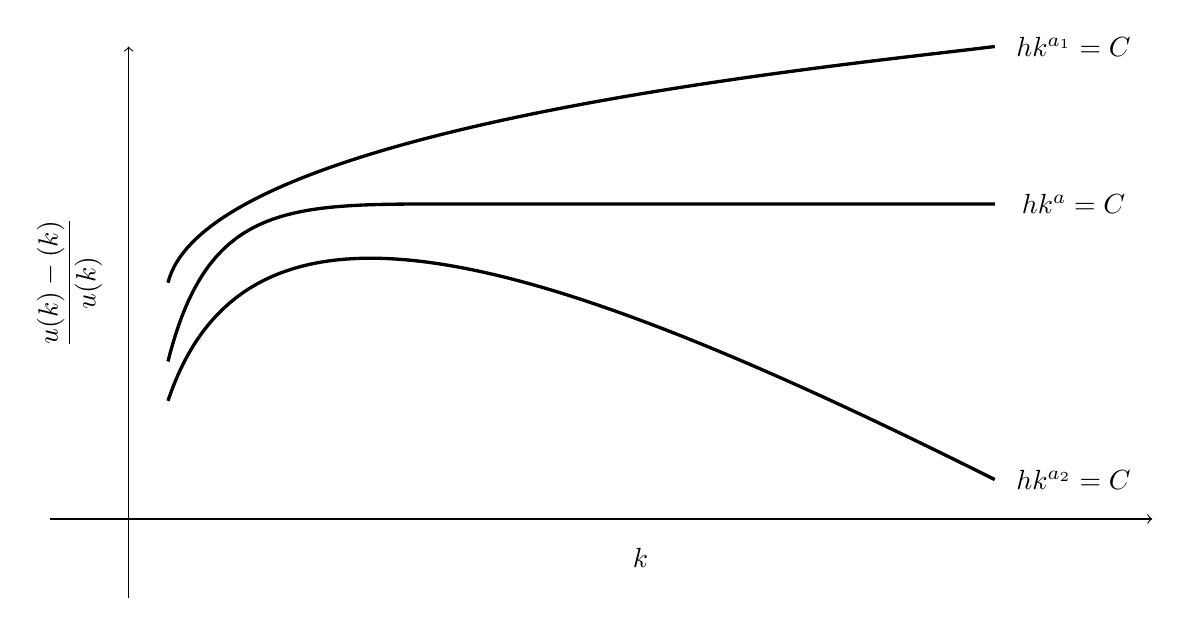
\begin{tikzpicture}
  
% axes
  
  \draw[->] (-1.0,0.0) -- (13.0,0.0);
  \draw[->] (0.0,-1.0) -- (0.0,6.0);

  \draw (6.5,-0.5) node {$k$};

  \draw (-0.75,3.0) node {\rotatebox{90}{$\displaystyle \frac{\NHokD{u(k)-\uh(k)}}{\NHokD{u(k)}}$}};
  % Found out about rotatebox from https://tex.stackexchange.com/a/45852

  

  % Good graph
  \draw[very thick] (0.5,2.0) .. controls (1.0,4.0) and (2.0,4.0) .. (4.0,4.0) -- (11.0,4.0);

  \draw (12.0,4.0) node {$hk^{a}=C$};

  % Bad graph
  \draw[very thick] (0.5,3.0) .. controls (1.0,5.0) and (9.0,5.75) .. (11.0,6.0);

    \draw (12.0,6.0) node {$hk^{a_{1}}=C$};

  % Overgood graph
    \draw[very thick] (0.5,1.5) .. controls (1.5,4.5) and (5.0,3.5) .. (11.0,0.5);

        \draw (12.0,0.5) node {$hk^{a_{2}}=C$};
  
  \end{tikzpicture}

\caption[A schematic of the expected behaviour of an $\hka{a}$-accurate finite-element method.]{A schematic of the expected behaviour of an $\hka{a}$-accurate finite-element method, when $hk^{a_1} = C,$ $hk^{a} = C,$ and $hk^{a_2} = C,$ for $C>0$ chosen appropriately, where $0 < a_{1} < a < a_{2}.$\label{fig:dataaccuracyplot}}
\end{figure}


\bre[$\hka{a}$-Quasi-optimality implies (better than) $\hka{a}$-data-accuracy]
Observe that, under standard assumptions on $u$, if the finite-element method is $\hka{a}$-quasi-optimal, then it is $\hka{a}$-data-accurate. We show this fact in the first order case, i.e., we take $p=1$ and $a=2.$ We assume $\NHtD{u} \leq\CHt k\NLtD{f}$ for some $k$-independent constant $\CHt>0$ (see, e.g., \cite[Lemma 2.12]{GaGrSp:15} for a setting in which this bound holds), and refer to  \cref{tab:qo} below for references for the fact that the first-order finite-element method is usually $\hka{2}$-quasi-optimal.

We show, in fact, that the finite-element method is $\hk{2}{1}$-data-accurate. If $hk^2 \leq \Co$ (where $\Co$ is given in the definition of $\hka{2}$-quasi optimality), then
\begin{align}
  \NHokD{u-\uh} &\leq \Cqo \NHokD{u-\uhptilde}\text{ where } \uhptilde \text{ is the approximation in \cref{lem:scottzhang},}\nonumber\\
  &\leq \Cqo \mleft(\NHoD{u-\uhptilde} + k\NLtD{u-\uhptilde}\mright)\nonumber\\
  &\leq \Cqo \CSZfn{2} \mleft(h\NHtD{u} + h^2k\NHtD{u}\mright) \text{ by \cref{lem:scottzhang},}\nonumber\\
    &\leq \Cqo \CSZfn{2}\CHt\mleft(hk + h^2k^2\mright)\NLtD{f}.\label{eq:qobetter}
\end{align}
Therefore, for $\eps \in (0,1)$ we define
\beqs
\Ct(\eps) = \frac1{\Cqo \CSZfn{2}\CHt} \min\set{\eps,\sqrt{\eps}}.
\eeqs
\ere
Hence if $hk^2 \leq \Co$ and $hk \leq \Ct,$ then $\NHokD{u-\uh}/\NLtD{f} \leq \eps,$ i.e. the finite-element method is $\hk{2}{1}$-data-accurate (and therefore if $k \geq\kz>0$ the finite-element method is $\hka{2}$-data-accurate, because $hk\lesssim hk^2$).

Observe, however, that the finite-element method is actually \emph{better than} $\hka{2}$-data-accurate, because the finite-element error \emph{decreases} as $k$ increases. With the above choices for $\Co,$ $\Ct,$ and $h$, from \cref{eq:qobetter} we have
\beqs
\NHokD{u-\uh} \leq \Cqo \CSZfn{2} \mleft(\frac{\Co}{k} + \frac{\Co^2}{k^2}\mright)\NLtD{f} \rightarrow 0 \quad\tas k \rightarrow \infty.
\eeqs
I.e., because we only need $hk$ sufficiently small to bound the interpolation error, but have taken $hk^2$ sufficiently small to ensure quasi-optimality, the finite-element error decreases as $k \rightarrow \infty.$


\bre[Relationship between $\hk{a}{b}$-accuracy and $\hk{a}{b}$-data-accuracy]\label{rem:accuracy}

\

The only difference between the definitions of $\hk{a}{b}$-accuracy and $\hk{a}{b}$-data-accuracy is that in \cref{eq:hkacc} the error is measured relative to the solution $u$, whereas in \cref{eq:hkdataacc} the error is measured relative to the `data' $f$ and $\gI$. However, if an a priori bound such as \cref{eq:tedpbound} holds, then $\hk{a}{b}$-accuracy implies $\hk{a}b$-data-accuracy, since $\NHokD{u} \lesssim \NLtD{f} + \NLtGI{\gI}$.

On the other hand, to conclude $\hk{a}{b}$-accuracy from $\hk{a}b$-data-accuracy, one would need to show the physically realistic criterion
\beq\label{eq:reversebound}
\NLtD{f} \lesssim \NHokD{u}.
\eeq
However, in general \cref{eq:reversebound} does not hold (as one can see by taking the unphysical solution $u=e^{ik^2 \bx}\chi,$ where $\chi$ is a smooth cut-off function; in this case $f = -\mleft(\Lap u + k^2 u\mright) \sim k^4,$ but $\NHokD{u} \sim k^2$). Therefore one cannot, in general, conclude $\hk{a}{b}$-accuracy from $\hk{a}{b}$-data-accuracy.
\ere

\bre[The above conditions for heterogeneous problems]\label{rem:accuracyhetero}
For a heterogeneous problem, the constants $\Co, \Ct$, and $\Cqo$ in \cref{def:hkacc,def:hkdataacc,def:hkqo} will all depend on the coefficients $A$ and $n.$ In general, this dependence is unknown. However, in \cref{sec:fem} below we prove that the $h$-finite-element method with polynomial degree $p$ is $\hka{(2p+1)/(2p)}$-data-accurate, where the dependence of $\Co$ and $\Ct$ on $n$ is completely known.
\ere

\bre[Generalisations of $\hk{a}{b}$-data-accuracy]
For discretisations of other Helmholtz problems (e.g., full-space problems with no truncation boundary $\GI$, or problems truncated with a perfectlly matched layer (PML)), then the denominator in \cref{eq:hkdataacc} should be adapted appropriately, e.g., the denominator should equal $\NLtD{f}$ for full-space problems and PML problems. In our discussion of the literature below (which includes such problems), we will make such an adaption without comment.
\ere




\subsubsection{Optimal mesh conditions for the finite-element method}

We now provide a brief overview of the optimal values of $a$ and $b$ for $\hk{a}{b}$-accuracy, $\hk{a}{b}$-data-accuracy, and $\hka{a}$-quasi-optimality. By `optimal', we mean the values of $a$ and $b$ that are smallest, corresponding to the least restrictive conditions on the mesh size $h$. We also, where possible, comment on whether these optimal conditions have been shown to be sharp. The literature reviews in this, and the next, section draw heavily on the literature reviews in \cite[pp. 182--183]{GrLoMeSp:14} and \cite[p. 112]{DiMoSp:19}. Unless otherwise stated, all the problems treated in this literature review are nontrapping (in the wider sense discussed under `\techtitle' in \cref{sec:wpdisc}), have constant coefficients, and have a impedance boundary condition on at least part of the boundary.

\bre[$hp$-methods for the Helmholtz equation]
We briefly mention the mesh conditions one obtains for $hp$-finite-element methods, even though they are not the focus of this thesis. The landmark results on $hp$-finite-element methods for the Helmholtz equation were achieved by Melenk and Sauter \cite{MeSa:10,MeSa:11} who used a novel splitting of the solution of the Helmholtz equation (see the comments at the start of \cref{sec:decomp} below) to show that the $hp$-finite-element method is quasi-optimal if $hk/p \leq \co$ and $p \geq \ct \ln k$ (for some constants $\co,\ct>0$). Melenk and Sauter proved this result for the full-space problem in \cite{MeSa:10} and for: (i) the exterior Dirichlet problem, and (ii) the interior impedance problem in an analytic domain or a 2-d convex polygon in \cite{MeSa:11}. These results were generalised to an arbitrary 2-d Lipschitz polygon by Esterhazy and Melenk in \cite[Theorem 4.2]{EsMe:12}. Other results in the literature for $hp$-finite-element methods are those of Zhu and Wu \cite[Equation (1.7)]{ZhWu:13} who showed the $hp$-finite-element method for the Helmholtz equation is data-accurate\footnote{We do not use the $\hk{a}b$-accurate, etc., terminology for $hp$-methods, as it does not represent the interplay between the polynomial degree $p$ and the wavenumber $k$.} provided
\beqs
\frac{kh}p \leq C_0\mleft(\frac{p}k\mright)^{\frac1{p+1}},
\eeqs
where $C_0>0$ is some constant.% Finally, in \cite[Corollary 3.2]{IhBa:97} Ihlenburg and Babu\v{s}ka proved a bound on the error for the finite-element method in 1-d that is explicit in $k,$ $h$, and $p$, although the bound is probably not sharp in $p,$ and therefore could not be used to prove results on $hp$-finite-element methods.
\ere


\paragraph{$\hk{a}b$-accuracy} In 1-d the $h$-finite-element method has been proved to be $\hka{3/2}$-accurate for first-order finite elements by Ihlenburg and Babu\v{s}ka in \cite[Theorem 5 and Equation (3.25)]{IhBa:95a} and \cite[Equation (4.5.15)]{Ih:98}. For higher-order finite-elements (still in 1-d) they proved the $h$-finite-element method is $\hka{(2p+1)/(2p)}$-accurate in \cite[Corollary 3.2]{IhBa:97} and \cite[Theorem 4.27 and Equation 4.7.41]{Ih:98}. However, all the above results were only measured in the $H^1$ seminorm (and so we are slightly abusing the notation of $\hka{a}$-accuracy here), and the higher-order results were proved under the assumptions that $f \in \HpmoD,$ $u \in \HppoD,$ and $\SNHppoD{u} \sim k^p \SNHoD{u}.$

These $\hka{a}$-accuracy results were confirmed numerically (for $p=1$) to be sharp by \cite[Figure 11]{IhBa:95a} and \cite[Figure 4.13]{Ih:98}, which showed that the relative error is bounded if $h \sim k^{-3/2}$ and by \cite[Figure 4.10]{Ih:98}, which showed that the relative error is not bounded if $h \sim k^{-1}.$

These results were proved using the properties of the `discrete Green's function' for the Helmholtz equation. This function was used to first prove an a priori bound on the finite-element approximation of the solution, and the error bounds were then concluded from this a priori bound. Furthermore, the higher-order proofs in \cite{IhBa:97,Ih:98} showed the finite-element error was bounded by $\SNHppoD{u}$, and then used the fact that
\beq\label{eq:ratio1d}
\frac{\SNHppoD{u}}{\SNHoD{u}} \sim k^p
\eeq
to bound the finite-element error by $\SNHoD{u},$ and hence conclude a bound on the relative error. The relation \cref{eq:ratio1d} follows because the solution of the Helmholtz equation in 1-d is given by
\beq\label{eq:soln1d}
A \cos(kx) + B \sin(kx)
\eeq
(for some constants $A$ and $B$).

As the discrete Green's function is only known explicitly in 1-d, and because \cref{eq:soln1d} only holds in 1-d (and therefore one can, in general, only prove \cref{eq:ratio1d} in 1-d), the proofs of $\hka{a}$-accuracy have not been extended to higher dimensions, although we conjecture they are true.  The only computational results for higher dimensions are those by Bayliss, Goldstein, and Turkel, who observed in \cite[Section 3, Tables 1--3]{BaGoTu:85} that, for low wavenumbers $k \in (4.16,8.32)$ the relative error for first-order finite-elements is bounded if $h \sim k^{-3/2}$, but is not bounded if $h \sim k^{-1}.$

\paragraph{$\hk{a}b$-data-accuracy} The best results known to date are the same (in terms of $a$ and $b$) as those for $\hk{a}b$-accuracy, except results for $\hk{a}b$-data-accuracy hold in higher dimensions. In \cite[Theorem 5.1, Corollary 5.2]{DuWu:15} Du and Wu essentially proved that the $h$-finite-element method for the IIP is $\hka{(2p+1)/(2p)}$-data-accurate for arbitrary (fixed) polynomial degree $p$ and $d = 2$ or $3$, provided $u \in \HppoD$ (although this result can be shown for lower-regularity solutions by combining \cite[Theorem 5.1]{DuWu:15} with \cite[Lemma 3.5]{DuWu:15}). This result was proved for the IIP in $d = 2$ or $3$ for $p=1$ by Wu in \cite{Wu:14}. We recall from \cref{rem:accuracy} that in physically realistic cases where \cref{eq:reversebound} holds, $\hk{a}{b}$-data-accuracy implies $\hk{a}{b}$-accuracy.

%The only computational evidence we know that in some way  confirms the sharpness of this result is that of Chaumont-Frelet and Nicaise \cite[Section 6.3, Figure 9]{ChNi:18}. They show that for scattering by a re-entrant corner, the relative $L^2$-error is bounded independently of $k$ provided $h^{2p}k^{2p+1}$ is bounded, for $p = 1,2,$ and $6.$ However, in general the result for $\hk{a}b$-data-accuracy coincides with the (sharp) best case for $\hk{a}b$-accuracy (in terms of the valuyes of $a$ and $b$), and so we expect the result for $\hk{a}b$-data-accuracy is also sharp.


\paragraph{$\hka{a}$-quasi-optimality} The best known result for $\hka{a}$-quasi-optimality for the Helmholtz equation is that the $h$-finite-element method is $\hka{(p+1)/p}$-quasi-optimal. This was first proved for $p=1$ in 1-d by Aziz, Kellog, and Stevens in \cite[Theorem 3.1]{AzKeSt:88} and Ihlenburg and Babu\v{s}ka in \cite[Theorem 3]{IhBa:95a} and \cite[Theorems 4.9 and 4.13]{Ih:98}, with \cite[Figures 7-9]{IhBa:95a} and \cite[Section 4.5.4 and Figures 4.11-4.12]{Ih:98} showing this result is sharp in 1-d (although Ihlenburg and Babu\v{s}ka only work in the $H^1$-semi norm). The result was proved for $p=1$ and $d=2$ for the IIP by Melenk \cite[Proposition 8.2.7]{Me:95}, and for higher-order finite elements (for the full-space problem, IIP, and EDP) by Melenk and Sauter in \cite[Corollary 5.6]{MeSa:10} and \cite[Theorem 5.8]{MeSa:11} respectively. This result was shown for a PML problem by Chaumont-Frelet, Gallistl, Nicaise, and Tomezyk in \cite[Theorem 5.1]{ChGaNiTo:18}, and extended to a class of time-harmonic wave propagation problems by Chaumont-Frelet and Nicaise in \cite[Theorem 2.15]{ChNi:19}, who showed that if the constant in the a priori bound \cref{eq:bgbound} grows like $k^\alpha,$ then the $h$-finite-element method is $\hka{(p+\alpha+1)/p}$-accurate. They give numerical experiments in \cite[Figure 8]{ChNi:19} showing the sharpness of $\hka{(p+1)/p}$-quasi-optimality for $p=1, 2$ for a heterogeneous IIP.

\paragraph{Link with dispersion error} When computing on regular grids, one can mathematically analyse the `dispersion error' of the finite-element method for the Helmholtz equation; i.e., the difference between the wavenumber of the true solution $u$ (i.e., $k$) and the wavenumber of the approximation $\uh.$ We mention briefly that Ainsworth  analysed the dispersion error for the $hp$-finite-element method for the Helmholtz equation and proved the dispersion error is of the order $h^{2p}k^{2p+1}$ \cite[Equation (3.5)]{Ai:04} (cited in \cite[Remark 5.3(a)]{DuWu:15}). Observe that this is the same order as the best-available results for $\hka{a}$-accuracy and $\hka{a}$-data-accuracy discussed above. Therefore, results from finite-element error analysis and dispersion analysis both suggest that the error (measured in a suitable sense in each case) is bounded if $h^{2p}k^{2p+1}$ is sufficiently small. See, e.g., \cite[Remark 5.3(a)]{DuWu:15} for more references on dispersion error analysis for the Helmholtz equation.

\bre[Comparison with $hp$-finite-element methods]
Observe that the optimal results for higher-order finite elements become less stringent as $p$ increases, i.e., the finite-element method is $\hka{(2p+1)/(2p)}$-data-accurate, and $(2p+1)/(2p) \downarrow 1$ as $p \rightarrow \infty.$ Therefore, in the $p\rightarrow \infty$ limit, we recover the mesh condition `$hk$ is sufficiently small'; that is, a fixed number of points per wavelength (recall the discussion on page \pageref{page:ppw} above).

Observe that the mesh condition `$hk$ is sufficiently small' implies that the number of degrees of freedom in the resulting linear systems is of the order $k^d.$ This same scaling for the number of degrees of freedom is obtained for $hp$-methods for the Helmholtz equation, see \cite[Remark 5.9]{MeSa:11}. Therefore, in the $p\rightarrow\infty$ limit, the number of degrees of freedom required for the $h$-finite-element method scales optimally, as for the $hp$-finite-element method.
\ere

%\paragraph{Observations} Observe that, in general, the mesh conditions required for quasi-optimality are more restrictive than those required for the error to be bounded. I.e., in general, if the finite-element method is both $\hka{\ao}$-quasi-optimal and $\hka{\at}$-data-accurate, then one sees that $\ao > \at$ (compare the entries in \cref{tab:acc,tab:dataacc} with those in \cref{tab:qo}). Therefore, whilst one can show the finite-element method is $\hka{a}$-data-accurate (for some $a$) by first showing quasi-optimality, this approach will result in a more restrictive mesh condition than proving $\hka{a}$-data-accuracy directly. Also 

\subsubsection{Complete summary of results in the literature}

In \cref{tab:acc,tab:dataacc,tab:qo} we list all of the mathematical (as opposed to computational) results in the literature for $\hk{a}b$-accuracy, $\hk{a}b$-data-accuracy, and $\hka{a}$-quasi-optimality. We list these in chronological order, with any relevant comments in the `Notes' column. The `Proof technique' column details the method used in the proof; see \cref{sec:prooftechniques} below for an extended discussion of these techniques. However, we now make a few general comments on the history of these results.

\paragraph{Lack of coercivity} Recall that proving quasi-optimality (or an error bound) for the finite-element method for the Helmholtz equation is more difficult than for the stationary diffusion equation \cref{eq:stdiff}. For the stationary diffusion equation, one immediately obtains quasi-optimality for \emph{any} mesh by C\'ea's Lemma (and one then obtains that the relative error is bounded by \cref{lem:scottzhang}). We emphasise again that this result holds for any shape-regular mesh, with no restriction on $h.$

However, C\'ea's Lemma relies on the coercivity of the sesquilinear form, and the sesquilinear forms arising from standard discretisations of the Helmholtz equation are not coercive for large $k$. Therefore, to prove quasi-optimality, one instead uses the so-called Schatz argument, a modification of the standard Aubin--Nitsche duality argument\footnote{First introduced by Aubin \cite{Au:67} and Nitsche \cite{Ni:68} for coercive problems.} However, using the Schatz argument, one only obtains quasi-optimality under some $k$-dependent restriction on the mesh size $h.$

\paragraph{Quasi-optimality using the Schatz argument} The Schatz argument was first used for problems satisfying a G\r{a}rding inequality by Schatz \cite{Sc:74} and first used for Helmholtz problems by Aziz, Kellogg, and Stephens \cite{AzKeSt:88}. In \cite{AzKeSt:88} they proved that in 1-d the finite-element method for the Helmholtz equation is $\hka{2}$-quasi-optimal, and this result was extended to $d=2$ by Melenk \cite{Me:95} in his PhD thesis. However, the Schatz argument was first presented in the framework we use below by Sauter \cite[Section 2]{Sa:06}. Observe that for large values of $k,$ $\hka{2}$-quasi-optimality and the related mesh restriction `$hk^2$ is sufficiently small' is computationally prohibitive---it would result in linear systems of size, e.g., $~10^{12}$, for the Helmholtz equation with $k=100$ in 3-d.

\paragraph{Error bounds using elliptic projections} Because of the severe mesh restrictions required for quasi-optimality for Helmholtz problems, recent research efforts have been focused on directly proving error bounds for the finite-element method. The key proof techniques are so-called elliptic projection ideas; these ideas are at the heart of our results in \cref{sec:fem} below, and are discussed in more detail in \cref{sec:prooftechniques} below. To our knowledge, the first use of elliptic projections to prove error estimates for Galerkin approximations was by Wheeler\footnote{Mentioned in \cite{MaNo:03}.} \cite[Theorem 3.1 ff.]{Wh:73}, who proved bounds on the error for a nonlinear parabolic problem by splitting the error into the error from an elliptic projection and the remaining error between the elliptic projection and the Galerkin approximation. The idea of using elliptic projections for Helmholtz problems was first introduced to prove error bounds for discontinuous Galerkin methods for \cref{prob:tedp} by Feng and Wu \cite{FeWu:09,FeWu:11}, and then used for standard finite-element methods (or closely-related continuous-interior-penalty methods) beginning with the work of Wu and Zhu \cite{ZhWu:13,Wu:14}.

\afterpage{% Heard about from https://tex.stackexchange.com/questions/11471/how-to-wrap-text-around-landscape-page
\begin{landscape} % Heard about from https://tex.stackexchange.com/questions/19017/how-to-place-a-table-on-a-new-page-with-landscape-orientation-without-clearing-t/19021#19021 and https://tex.stackexchange.com/questions/25369/how-to-rotate-a-table 
\begin{table}[h]
  \centering
  \begin{threeparttable}[c]
    \begin{tabular}{Sc Sc Sc Sc}
  \toprule
  & $\hk{a}b$-accuracy & Notes & Proof technique\\
   \midrule
    \cite[Equation (3.25)]{IhBa:95a} & $\displaystyle\hk{1}{\frac32}$ & \makecell{$d=1$, unit interval,\\$u(0)=0,$\\impedance boundary condition at $1$\\$H^1$ seminorm}&\makecell{Discrete Green's function\\(specific to $d=1$)}\\
    \cite[Theorem 4]{IhBa:95b} & $\displaystyle\hk{1}{\frac32}$ & \makecell{$d=1$, unit interval,\\$u(0)=0,$\\impedance boundary condition at $1$\\$L^2$ norm\tnote{1}}&\makecell{Discrete Green's function\\error splitting using interpolant}\\
      \cite[Corollary 3.2]{IhBa:97}&$\displaystyle\hk{1}{\frac{2p+1}{2p}}$ & \makecell{$d=1$, unit interval,\\$u(0)=0,$\\impedance boundary condition at $1$\\$H^1$ seminorm}&\makecell{Discrete Green's function,\\error splitting using interpolant}\\
  \cite[Theorem 4.13 and equation (4.5.15)]{Ih:98}& $\displaystyle\hk{1}{\frac32}$ & \makecell{$d=1$, unit interval,\\$u(0)=0,$\\impedance boundary condition at $1$\\$H^1$ seminorm}& Discrete Green's function\\
  \cite[Theorem 4.27 and equation (4.7.41)]{Ih:98}& $\displaystyle\hk{1}{\frac{2p+1}{2p}}$ & \makecell{$d=1$, unit interval,\\$u(0)=0,$\\impedance boundary condition at $1$\\$H^1$ seminorm}&\makecell{Discrete Green's function,\\error splitting using interpolant}\\ 
  \bottomrule
  \end{tabular}
  \begin{tablenotes}
\item [1] Actually, \cite[Theorem 4]{IhBa:95b} only proves a bound on the $L^2$-norm of the error in terms of the $H^2$-seminorm of the solution. However, when $d=1$, $\SNHtD{u} \sim k^2\NLtD{u}$ and so one can conclude $\hk{a}b$-accuracy.
  \end{tablenotes}
    \caption{All the results in the literature on $\hk{a}b$-accuracy for $h$-finite-element discretisations of the Helmholtz equation.}\label{tab:acc}
\end{threeparttable}
\end{table}

\begin{table}[h]
  \centering
\begin{tabular}{Sc Sc Sc Sc}
  \toprule
 & $\hk{a}b$-data-accuracy  & Notes & Proof technique\\
  \midrule
  \cite[Lemma 2.6]{DoSaShBe:93} & $\displaystyle\hka{\frac32}$ & \makecell{$d=1$, unit interval,\\impedance boundary condition at both endpoints}&Modified Schatz \\
  \cite[Theorem 5]{IhBa:95a} & $\displaystyle\hk{1}{\frac32}$ & \makecell{$d=1$, unit interval, $u(0)=0,$\\impedance boundary condition at $1$}&\makecell{Discrete Green's function\\error splitting using interpolant}\\
      \cite[Corollary 4.2]{ZhWu:13}& $\displaystyle\hk{\frac{p+2}{p+1}}{\frac{2p+1}{2p}}$   &\makecell{$d=2,3$, IIP, $D$ smooth,\\bounds obtained for $hp$-finite-element method,\\so fully $p$-explicit}& Modified Schatz\\
      \cite[Theorem 5.1]{Wu:14} & $\hka{3/2}$  &\makecell{$d=2,3$, IIP,\\$D$ a star-shaped polygon/polyhedron}& Error splitting\\
      \cite[Corollary 5.2]{DuWu:15} & $\displaystyle\hka{\frac{2p+1}{2p}}$ &  $d=2,3$, IIP, $D$ smooth, star-shaped& Error splitting\\
        \cite[Theorem 5.5]{ChNi:18}& $\displaystyle\hk{\frac{3+\sigma}{1+\alpha}}{3/2}$   &\makecell{$d=2$, TEDP with re-entrant corners,\\a priori bound grows like $k^\sigma$, $\alpha \in (1/2,1)$\\related to strength of corner singularities}& Modified Schatz\\
        \pbox{3.2cm}{\cite[Theorem 4.4 and Remark 4.5(iv)]{LiWu:19}}& $\hka{3/2}$   &\makecell{$d = 1,2,3$, full-space problem truncated with PML,\\posed in a ball}& Modified Schatz\\
        \cite[Lemma 3.3]{WuZo:18}&$\hka{3/2}$&\makecell{IIP, $D$ convex,\\$n$ heterogeneous with $\NLiDRR{n-1} \lesssim 1/k$,\\part of an argument for a\\nonlinear heterogeneous Helmholtz problem}&Error splitting\\
  \cite[Theorem 5.4]{ChGaNiTo:18}&$\displaystyle\hk{\frac{p+2}{p+1}}{\frac{2p+1}{2p}}$  & \makecell{$d=2$, EDP truncated with PML,\\posed in a ball}& Modified Schatz\\
\bottomrule
\end{tabular}
\caption{All the results in the literature on $\hk{a}b$-data-accuracy for $h$-finite-element discretisations of the Helmholtz equation.}\label{tab:dataacc}
\end{table}


  \begin{table}[h]
    \centering
      \begin{threeparttable}[c]
\begin{tabular}{Sc Sc Sc Sc}
  \toprule
& $\hka{a}$-quasi-optimality & Notes & Proof technique\\
  \midrule
  \cite[Theorem 3.1]{AzKeSt:88} & $\hka{2}$ & $d=1$ & Schatz\\
  %?  \cite{DoSaShSc:93}\\
  \cite[Theorem 3]{IhBa:95a} & $\hka{2}$ & $d=1,$ $H^1$ seminorm & Schatz\\
  \cite[Corollary 2]{IhBa:95a} & $\hka{2}$ & $d=1,$ $H^1$ seminorm &\makecell{Discrete Green's function,\\error splitting using interpolant\tnote{1}}\\
  %? \cite{IhBa:95b}
  \pbox{3.5cm}{\cite[Theorems 4.9 and 4.13]{Ih:98}} & $\hka{2}$ & \makecell{$d=1,$ $H^1$ seminorm,\\\cite[Theorem 4.9]{Ih:98} is \cite[Theorem 3]{IhBa:95a}} & \makecell{Schatz and error splitting\\using interpolant, respectively}\\
  \cite[Proposition 8.2.7]{Me:95} & $\hka{2}$ & \makecell{$d=2,$ IIP, $D$ smooth and star-shaped or convex} & Schatz\\
  \cite[Corollary 5.6]{MeSa:10} & $\displaystyle\hka{\frac{p+1}p}$ & Full-space problem & Schatz\\
%  \cite[Theorem 5.8]{MeSa:11} & $\hka{(p+1)/p}$ & \makecell{$d = 2,3$,\\polynomial growth of constant in a priori bound,\\IIP ($\Dm$ analytic or Lipschitz convex polygon)\\and EDP ($\Dm$ analytic)} & Schatz\\
  \cite[Theorem 5.3]{ChNi:18} & $\hka{2+\sigma}$ & \makecell{$d=2$, TEDP with re-entrant corners\\a priori bound grows like $k^\sigma$} & Schatz\\
  \cite[Theorem 5.1]{ChGaNiTo:18} & $\displaystyle\hka{\frac{p+1}p}$&$d=2$, EDP truncated with PML, posed in a ball  &Schatz\\
    \cite[Theorem 2.15]{ChNi:19} & $\displaystyle\hka{\frac{p+\alpha+1}p}$ & \makecell{Class of time-harmonic wave problems,\\a priori bound grows at rate $k^\alpha$} & Schatz\\
    \pbox{3.5cm}{\cite[Theorems 4.2 and 4.5, Remark 4.6(ii)]{GrSa:18}} &$\hka{2}$ & \makecell{IIP, $D$ Lipschitz, star-shaped w.r.t. a ball,\\$n$ heterogenenous, constants fully explicit in $n$}& Schatz\\
    \cite[Theorem 3]{GaSpWu:18} & $\hka{2}$ & \makecell{EDP, $A$ and $n$ heterogeneous, $\Dm,$ $A$, and $n$ $C^\infty$,\\constants fully explicit in $A$ and $n$} & Schatz\\
\bottomrule
\end{tabular}
  \begin{tablenotes}
\item [1] Actually, \cite[Corollary 2]{IhBa:95a} proves  quasi-optimality with contstant proportional to $k$ if $hk$ is sufficiently small.
  \end{tablenotes}
  \caption{All the results in the literature on $\hka{a}$-quasi-optimality for $h$-finite-element discretisations of the Helmholtz equation.}\label{tab:qo}
  \end{threeparttable}
\end{table}
\end{landscape}
}


\subsection{Extended discussion of proof techniques for finite-element errors for the Helmholtz equation}\label{sec:prooftechniques}
We now discuss in some detail the proof techniques used to obtain either $\hk{a}b$-accuracy, $\hk{a}b$-data-accuracy, or $\hka{a}$-quasi-optimality. We note that frequently quasi-optimality results are refereed to as \defn{asymptotic} error estimates, and accuracy or data-accuracy results (when they are proved under weaker mesh constraints than asymptotic estimates) are referred to as \defn{pre-asymptotic} error estimates. This terminology is used because the mesh conditions to ensure quasi-optimality are more restrictive than those for bounded error, and therefore they hold only for smaller values of $h.$

For simplicity, our exposition below will assume that we are treating \cref{prob:vtedp} with homogeneous coefficients (i.e., $A=I$ and $n=1$) with $\gI = 0,$ and that the problem is nontrapping\footnote{Recall that we say that the problem is nontrapping if $C$ in \cref{eq:bgbound} is bounded independent of $k,$ for $k \geq \kz$.}, and therefore in particular the solution $u$ of \cref{prob:vtedp} is unique. Also, we suppress all of the constants involved, instead opting to use $\lesssim$ notation, where $a \lesssim b$ if $a \leq C b,$ with $C$ independent of $k$ and $h$. The new results we present in \cref{thm:fembound} consider heterogeneous problems that may be trapping, and state all of the constants involved explicitly, at the price of being more technical to state.

\subsubsection{Comparison of the different classes of argument}
We first briefly discuss the positive and negative points for each of the two classes of argument we will outline below: (modified) duality arguments and error-splitting arguments.

The merits of duality arguments are their simplicity---we will state the arguments in their entirety in this overview section. Moreover, the mesh conditions and error bounds one obtains are completely $h$-, $p$-, and $k$-explicit. However, the main drawback of duality arguments (when used to prove data-accuracy) is their lack of sharpness in the conditions imposed on $h$, see, e.g., the discussion in \cref{rem:dataacc} above.

In contrast, the merit of error-splitting arguments is that they can give mesh conditions that are sharp in their $h$-dependence; in \cite{DuWu:15}, Du and Wu proved that the finite-element method is $\hka{(2p+1)/2p}$-data-accurate, i.e., the mesh restriction needed for existence and uniqueness of $\uh$ is \emph{of the same order} as the mesh restriction needed to bound the finite-element error uniformly in $k.$

However, the drawback of error-splitting arguments is their complexity. They involve proving bounds on the solution of discrete Helmholtz problems; such bounds are complicated to prove, especially in the higher-order cases, and the constants involved depend on the polynomial degree $p$ in highly complicated ways. These drawbacks limit the likelihood that such bounds can be used for $hp$-finite-element methods, where the dependence on the polynomial degree must be known explicitly.


\subsubsection{(Modified) duality arguments}
These arguments are used to prove quasi-optimality and data-accuracy results; they include the more commonly known Schatz argument for Helmholtz problems. We first give the Schatz argument (for proving quasi-optimality), before going on to outline modified Schatz arguments (for proving data-accuracy).

Before we proceed we establish some notation that will enable us to discuss best approximation errors for solutions of Helmholtz problems. We let $\solfem:\LtD\rightarrow \HoD$ denote the solution operator for \cref{prob:vtedp} with zero impedance boundary condition, and we let $\solfems$ denote the solution operator for the corresponding adjoint problem. That is, for any $\ftilde \in \LtD$ and for all $v \in \HozDD,$
\beqs
\aT(\solfem(\ftilde),v) = \IPLtD{\ftilde}{v}
\eeqs
and
\beqs
\aT(v,\solfems(\ftilde)) = \IPLtD{v}{\ftilde}.
\eeqs
We next define the approximability constants:
\beq\label{eq:wbadef}
\wba \de \sup_{\ftilde \in \LtD}\inf_{\vh \in \Vhp} \frac{\NHokD{\solfem(\ftilde) - \vh}}{\NLtD{\ftilde}}
\eeq
and
\beqs
\wbaadj \de \sup_{\ftilde \in \LtD}\inf_{\vh \in \Vhp} \frac{\NHokD{\solfems(\ftilde) - \vh}}{\NLtD{\ftilde}}.
\eeqs

Observe that the definitions of $\wba$ and $\wbaadj$ imply that for all $\ftilde \in \LtD$
\beq\label{eq:wbaimpl}
\inf_{\vh \in \Vhp} \NHokD{\solfem(\ftilde) - \vh} \leq \wba \NLtD{\ftilde}
\eeq
and
\beq\label{eq:wbaadjimpl}
\inf_{\vh \in \Vhp} \NHokD{\solfems(\ftilde) - \vh} \leq \wbaadj \NLtD{\ftilde}.
\eeq
We will use the bounds \cref{eq:wbaimpl,eq:wbaadjimpl} in the Schatz and modified Schatz arguments below.

When dealing purely with the Schatz argument for quasi-optimality (as in \cite[Section 2.2]{Sa:06}) one only needs to consider the approximation of adjoint problems in the duality-argument step, and hence one only needs $\wbaadj$. However, in our exposition of elliptic-projection-based arguments below, we will also need to consider the approximation of standard Helmholtz problems, and hence we introduce notation for both $\wba$ and $\wbaadj.$

 \paragraph{The Schatz argument for quasi-optimality} The first step is to use the G\r{a}rding inequality \cref{eq:gardingbrief} satisfied by the Helmholtz equation to show that the error in the weighted $H^1$ norm is bounded by the best approximation error, plus the error in the $L^2$ norm\footnote{Recall that for the stationary diffusion equation, one can show the finite-element error is bounded by the approximation error simply using coercivity and boundedness of the bilinear form---this is Cea's Lemma.}. We assume $\uh$ exists, and observe that by the G\r{a}rding inequality \cref{eq:gardingbrief} (with $\aT$ as in \cref{eq:aT})
\begin{align}
\NHokD{u-\uh}^2 &\leq \Re{\aT(u-\uh,u-\uh)} + k^2 \NLtD{u-\uh}^2\nonumber\\
&= \Re{\aT(u-\uh,u-\vh)} + k^2 \NLtD{u-\uh}^2\text{ by Galerkin orthogonality,}\nonumber\\
&\lesssim \NHokD{u-\uh}\NHokD{u-\vh} + k^2 \NLtD{u-\uh}^2,\label{eq:gardingerror}
\end{align}
for any $\vh \in \Vhp.$

We now use a modification of the standard Aubin--Nitsche duality argument to bound $\NLtD{u-\uh}$ by $\wbaadj \NHokD{u-\uh}$ (and recall that $\wbaadj$ can be made small). Let $\xi \in \HozDD$ solve the adjoint Helmholtz problem
\beq\label{eq:xidef}
\aT(v,\xi) = \IPLtD{v}{u-\uh} \tforall v \in \HozDD.
\eeq
Then, taking $v = u-\uh,$ we have
\begin{align}
  \NLtD{u-\uh}^2 &= \aT(u-\uh,\xi)\label{eq:schatz0}\\
  &=\aT(u-\uh,\xi - \vh) \text{ by Galerkin orthogonality for } u-\uh, \text{ for any } \vh \in \Vhp\nonumber\\
  &\lesssim \NHokD{u-\uh}\NHokD{\xi-\vh}\nonumber\\
  &\lesssim \NHokD{u-\uh} \wbaadj \NLtD{u-\uh}\text{ by \cref{eq:wbaadjimpl}.}\nonumber
\end{align}
Cancelling a factor of $\NLtD{u-\uh},$ we obtain
\beq\label{eq:schatz1}
\NLtD{u-\uh} \lesssim \wbaadj \NHokD{u-\uh}.
\eeq
Combining \cref{eq:gardingerror,eq:schatz1}, we have
\beqs
\NHokD{u-\uh}^2 \lesssim \NHokD{u-\uh}\NHokD{u-\vh} + \mleft(k\wbaadj\mright)^2 \NHokD{u-\uh}^2,
\eeqs
and hence by cancelling a factor $\NHokD{u-\uh}$ and taking the final term on to the left-hand side, we obtain
\beq\label{eq:qofinal}
\NHokD{u-\uh} \lesssim \inf_{\vh \in \Vhp} \NHokD{u-\vh} \tif k\wbaadj \text{ is sufficiently small}.
\eeq

All results showing quasi-optimality for the Helmholtz equation (for different finite-element spaces and different domains) can then be seen as simply obtaining estimates on $\wbaadj$ in these different scenarios; this literature is summarised in \cref{tab:qo}. For example, if $p=1,$ then one can show $\wbaadj \sim hk,$ and hence we can conclude the first-order finite-element method is $\hka{2}$-quasi-optimal.

We have just shown quasi-optimality under the assumption that $\uh$ exists. For proof of existence, we follow the proof of \cite[Theorem 5.21]{Sp:15}. Via the rank-nullity theorem (since \cref{eq:fevtedp} is equivalent to a finite-dimensional linear system) existence and uniqueness of $\uh$ are equivalent. We now show uniqueness of $\uh.$ By linearity, uniqueness of $\uh$ is equivalent to showing uniqueness of the solution of
\beqs\label{eq:uniqproof}
\aT\mleft(\uhtilde,\vh\mright) = 0 \tforall \vh \in \Vhp,
\eeqs
i.e., showing $\uhtilde = 0.$ Clearly $\uhtilde$ is a finite-element approximation of $\utilde \in \HozDD$, where $\utilde$ solves
\beqs
\aT\mleft(\utilde,v\mright) = 0 \tforall \vh \in \HozDD.
\eeqs
Since our problem is assumed nontrapping, it follows that $\utilde$ is unique, and hence $\utilde = 0$. Therefore \cref{eq:qofinal} becomes
\beq\label{eq:qofinaluniq}
\NHokD{\uhtilde} \lesssim \inf_{\vh \in \Vhp} \NHokD{\vh} \tif k\wbaadj \text{ is sufficiently small}.
\eeq
The right-hand side of \cref{eq:qofinaluniq} is 0, and therefore $\uhtilde=0.$ As outlined above, uniqueness of $\uh$ follows and therefore $\uh$ exists and is unique.

\paragraph{Modified Schatz arguments for data-accuracy} The main difference between the Schatz argument and modified Schatz arguments is that modified Schatz arguments only prove a \emph{bound} on the finite-element error, rather than proving quasi-optimality. Modified Schatz arguments (and error-splitting arguments, that we outline later) use the elliptic projection of a function. Therefore, we first outline the definition and some properties of elliptic projections.



The elliptic projection of a function $ w \in \HozDD$ is the finite-element function $\Ph w$ that has the same action as $w$ on the finite-element space $\Vhp$ with respect to a coercive and continuous sesquilinear form\footnote{The definition of the elliptic projection depends on the exact sesquilinear form used in the discretisation of the Helmholtz equation, and on the norm one is using to measure the error. For example, elliptic projection arguments for the Helmholtz equation originated in the study of discontinuous Galerkin methods for the Helmholtz equation (in \cite{FeWu:09,FeWu:11}); therefore the sesquilinear forms associated with the discretisation included penalty terms. These penalty terms were incorporated into the sesquilinear form $\aep$ and the norms used to measure the error also included these penalty terms. In the following exposition, we will work with standard finite-element discretisations of the Helmholtz equation and standard Sobolev norms, and so the elliptic projections we used will be based on this setting.}; i.e., $\Ph w$ is defined by
\beqs
\aep(\vh,\Ph w) = \aep(\vh,w) \tforall \vh \in \Vhp,
\eeqs
for some coercive and continuous sesquilinear form $\aep$. For \cref{prob:vtedp}, with sesquilinear form given by \cref{eq:aT}, choices for $\aep(\vo,\vt)$ used in the literature are either
\beq\label{eq:aepho}
\aep(\vo,\vt) = \IPLtD{\grad \vo}{\grad \vt},
\eeq
\beq\label{eq:aeplower}
\aep(\vo,\vt) = \IPLtD{\grad \vo}{\grad \vt} + \IPLtD{\vo}{\vt},
\eeq
or
\beq\label{eq:aepused}
\aep(\vo,\vt) = \IPLtD{\grad \vo}{\grad \vt} - ik\IPLtGI{\vo}{\vt}.
\eeq
These elliptic projections correspond to finding finite-element approximations of the solution of the PDEs
\begin{subequations}
  \label{eq:sda}
\begin{align}
  \Delta w &= F \tin D,\label{eq:sd1}\\
  w &= 0 \ton \GD,\tand\label{eq:sd2}\\
  \dn w &= 0 \ton \GI\label{eq:sd3};
\end{align}
\end{subequations}
\begin{subequations}
    \label{eq:sdb}
\begin{align}
  \Delta w + w&= F \tin D,\label{eq:sd4}\\
  w &= 0 \ton \GD,\tand\label{eq:sd5}\\
  \dn w &= 0 \ton \GI;\label{eq:sd6}
\end{align}
\end{subequations}
or
\begin{subequations}
    \label{eq:sdc}
\begin{align}
  \Delta w &= F \tin D,\label{eq:sd7}\\
  w &= 0 \ton \GD,\tand\label{eq:sd8}\\
  \dn w -ikw &= 0 \ton \GI\label{eq:sd9}
\end{align}
\end{subequations}
respectively, where $F$ is an appropriately chosen function. In the following exposition, we will assume $\aep$ is given by \cref{eq:aepused}, and to ease the exposition, we assume the solution of \cref{eq:sdc} is in $\HtD$. One can show in this case that the energy norm $\Nep{\cdot}$ corresponding to \cref{eq:aepused} is equivalent to the weighted $H^1$-norm $\NHokD{\cdot}$, with equivalence constants independent of $k$, i.e.,
\beq\label{eq:aepnormequiv}
\Nep{v} \sim \NHokD{v} \tforall v \in \HozDD,
\eeq
by the multiplicative trace inequality (\cref{thm:multiplicativetrace}) and the Poincar\'e--Friedrich's inequality (\cref{lem:poincare}). Since $\Ph$ is a Galerkin projection, one can show that in its energy norm , $\aep$ is coercive and continuous\footnote{For comment on showing coercivity and continuity for the other definitions of $\aep$, see \cref{rem:epdef} below.}, and hence $\Ph$ is quasi-optimal:
\beq\label{eq:epho}
\Nep{w-\Ph w} \lesssim \inf_{\vh \in \Vhp} \Nep{w-\vh}.
\eeq
Also, by the Aubin--Nitsche duality argument (since $\aep$ is coercive),
\beq\label{eq:eplt}
\NLtD{w-\Ph w} \lesssim h \Nep{w-\Ph w}.
\eeq

Combining \cref{eq:epho,eq:eplt} is a modification of the Schatz argument above. We first adopt the notation that, for $v \in \HozDD,$ the function $\Ih v \in \Vhp$ is the function achieving the infimum in \cref{eq:wbaimpl}. We assume $\uh$ exists, and start from \cref{eq:schatz0}, but instead of introducing an arbitrary $\vh \in \Vhp$ into the second argument, we instead introduce the elliptic projection $\Ph \xi$ by Galerkin orthogonality for $u-\uh$:
\newpage
\begin{align}
  \NLtD{u-\uh}^2 &= \aT(u-\uh,\xi-\Ph\xi)\nonumber\\
  &= \aep(u-\uh,\xi-\Ph\xi) - k^2\IPLtD{u-\uh}{\xi-\Ph\xi}\text{ by \cref{eq:aepused},}\nonumber\\
  &= \aep(u-\Ih u,\xi-\Ph\xi) - k^2\IPLtD{u-\uh}{\xi-\Ph\xi}\nonumber\\
  &\quad\quad\text{ by Galerkin orthogonality for }\xi-\Ph\xi,\nonumber\\
    & \lesssim \Nep{u-\Ih u}\Nep{\xi - \Ph\xi}- k^2\IPLtD{u-\uh}{\xi-\Ph\xi}\nonumber\\
  &\lesssim \wba \NLtD{f} \Nep{\xi-\Ph\xi} + k^2 \NLtD{u-\uh} \NLtD{\xi-\Ph\xi}\text{ by \cref{eq:aepnormequiv} and \cref{eq:wbaimpl},}\nonumber\\
  &\lesssim \wba \NLtD{f} \wbaadj \NLtD{u-\uh} + k^2 \NLtD{u-\uh} \NLtD{\xi-\Ph\xi}\nonumber\\
  &\quad\quad\text{ by \cref{eq:epho}, \cref{eq:aepnormequiv}, \cref{eq:xidef}, and \cref{eq:wbaadjimpl}}\nonumber\\
  &\lesssim \wba\wbaadj \NLtD{f}\NLtD{u-\uh} + k^2 \NLtD{u-\uh} h\wba \NLtD{u-\uh}\label{eq:schatz2}\\
  &\quad\quad\text{ by \cref{eq:eplt}, \cref{eq:epho}, \cref{eq:aepnormequiv}, and \cref{eq:wbaimpl}.}\nonumber
\end{align}
Therefore if $hk^2\wba$ is sufficiently small, the second term on the right-hand side of \cref{eq:schatz2} can be absorbed into the left-hand side, and cancelling a factor of $\NLtD{u-\uh},$ we obtain
\beq\label{eq:ep1}
k \NLtD{u-\uh} \lesssim k \wba\wbaadj \NLtD{f} \tif hk^2\wba \text{ is sufficiently small.}
\eeq
%this is \cref{eq:epbound}. %(We consider $k\NLtD{u-\uh}$ so as to compare with the quasi-optimality results above, as the $L^2$ term in $\NHokD{\cdot}$ is also multiplied by a factor $k$.)

To obtain a bound on the error in the weighted $H^1$ norm, we put \cref{eq:ep1} into \cref{eq:gardingerror} to get
\beqs
\NHokD{u-\uh}^2 \lesssim \NHokD{u-\uh}\NHokD{u-\vh} + \mleft(k\wba\wbaadj\mright)^2 \NLtD{f}^2,
\eeqs
and taking $\vh = \Ih v,$ by \cref{eq:wbaimpl} we have
\beqs
\NHokD{u-\uh}^2 \lesssim \NHokD{u-\uh}\wba\NLtD{f} + \mleft(k\wba\wbaadj\mright)^2 \NLtD{f}^2,
\eeqs
We then obtain for any $\eps > 0$ by Cauchy's inequality \cref{eq:cauchy}
\beq\label{eq:ep2}
\NHokD{u-\uh}^2 \lesssim \eps \NHokD{u-\uh}^2 + \frac1\eps\wba^2 \NLtD{f}^2 + \mleft(k\wba\wbaadj\mright)^2 \NLtD{f}^2.
\eeq
Taking $\eps$ sufficiently small, moving the first term on the right-hand side of \cref{eq:ep2} to the left-hand side, and taking a square root, we obtain
\beq\label{eq:ep3}
\NHokD{u-\uh} \lesssim\mleft(\wba  + k\wba\wbaadj\mright) \NLtD{f} \tif hk^2\wba\text{ is sufficiently small}.
\eeq

Finally, we conclude existence and uniqueness of $\uh$ using a similar argument to the one used for the Schatz argument above, except now we use the bound \cref{eq:ep3} with $f = 0$ to conclude uniqueness of $\uhtilde$.

By definition of $\wba$ \cref{eq:wbaimpl}, the term $\wba\NLtD{f}$ on the right-hand side of \cref{eq:ep3} is, up to a constant, the best-approximation error for $u$ (i.e., the error when one interpolates/quasi-interpolates $u$), and the term $k\wba\wbaadj$ is the \defn{pollution} term arising from the numerical method.%As for the quasi-optimality results above, we remark that different bounds on the finite-element error (for different finite-element space $\Vhp$ and different domains) can be thought of as proving bounds on $\eta$ in these different situations.
%\ednote{Both---I don't yet have a clear explanation of \emph{why} this works. Currently, it seems just like a trick to me. I don't know if that's an issue!}
\subsubsection{Error-splitting arguments}\label{sec:errorsplit}
The second class of arguments used in the literature are error-splitting arguments, used to prove accuracy and data-accuracy results. In these arguments the finite-element error is split using the elliptic projection of the solution $u$. To begin, we assume $\uh$ exists and make the observation that
\beqs\label{eq:split1}
u-\uh = \mleft(u-\Ph u\mright) + \mleft(\Ph u - \uh\mright)
\eeqs
and therefore
\beqs
\NHokD{u-\uh} \leq \NHokD{u-\Ph u} + \NHokD{\Ph u - \uh}.
\eeqs
An error bound for $u-\uh$ can therefore be obtained by proving an error bound for the elliptic projection error $u- \Ph u$ and proving a bound on the difference $\Ph u - \uh.$ The former can either be accomplished by showing quasi-optimality of the elliptic projection (as above) or by proving such an error bound directly. The first approach is taken in \cite{DuWu:15,ChGaNiTo:18,LiWu:19}, and the second approach is taken in \cite[Lemma 5.2]{FeWu:09}\footnote{Although the proof is only contained in \cite[Lemma 5.2]{FeWu:08}), \cite[Lemma 4.3]{FeWu:11}, and \cite[Lemma 4.2]{Wu:14}.}. In \cite{FeWu:09,FeWu:11,Wu:14} the bound on the elliptic projection error is proved by observing that the sesquilinear form $\IPLtD{\grad \vo}{\grad \vt}$ is coercive on $\HozDD$, and then also controlling the additional term arising from the impedance boundary condition.

To bound the difference $\Ph u - \uh,$ one first shows that it solves a deterministic Helmholtz problem:
For any $\vh \in \Vhp$ we have $\aT(u-\uh,\vh) = 0$ and $\aep(u-\Ph u,\vh) = 0$ by Galerkin orthogonality for $u-\uh$ and $u-\Ph u$ respectively\footnote{For the arguments in this \lcnamecref{sec:errorsplit}, we define the elliptic projection in the first argument, see \cref{eq:ellprojfirst} below.}. Therefore
\begin{align*}
  \aT(\Ph u - \uh,\vh) &= \aT(\Ph u - u,\vh) + \aT(u-\uh,\vh)\\
  &= \aT(\Ph u - u,\vh)\\
  &= \aep(\Ph u - u,\vh) - k^2\IPLtD{\Ph u - u}{\vh}\\
  &= - k^2\IPLtD{\Ph u - u}{\vh},
\end{align*}
that is, $\Ph u - \uh$ solves the \emph{discrete} Helmholtz problem
\beq\label{eq:vhhdisc}
\aT(\Ph u - \uh,\vh) = \IPLtD{\ftilde}{\vh} \tforall \vh \in \Vhp,
\eeq
where $\ftilde = -k^2\mleft(u-\Ph u\mright).$ One then uses this fact that $\Ph u - \uh$ satisfies a discrete Helmholtz problem to prove a bound on the difference $\Ph u - \uh$ directly.



All that remains to be discussed is how to prove the bound on $\Ph u - \uh$, using the fact that it solves the discrete Helmholtz problem \cref{eq:vhhdisc}. In \cite{FeWu:09,FeWu:11,Wu:14} a discrete multiplier argument is used to prove a bound on $\Ph u - \uh$, reminiscent of the multiplier arguments used to prove a priori bounds on Helmholtz problems in \cref{sec:pdetheory}. In \cite{DuWu:15} an argument using higher-order (discrete) norms is used in an argument conceptually similar to the modified duality arguments above; this argument is the heart of the proof in \cref{sec:fem} below. In essence the argument in \cite{DuWu:15} reduces to showing the bounds
\beq\label{eq:duwu1}
\NLtD{\Ph u - \uh} \lesssim \mleft(h + \mleft(hk\mright)^p\mright)\NHokD{u-\Ph u} + \mleft(h^{p+1}k^2 + h^{2p}k^{p+2}\mright)\Nfn{p-1,h}{\Ph u - \uh}
\eeq
and
\beq\label{eq:duwu2}
\Nfn{p-1,h}{\Ph u - \uh} \lesssim h^{2-p} \NHokD{u- \Ph u} + k^{p-1} \NLtD{\Ph u - \uh},
\eeq
where $\Nfn{p-1,h}{\cdot}$ is a discrete norm analogous to the Sobolev norm of order $p-1$. The bounds \cref{eq:duwu1,eq:duwu2} are then combined (under the assumption that $hk\lesssim 1$) to show
\beqs
\NLtD{\Ph u - \uh} \lesssim \mleft(h + \mleft(hk\mright)^p\mright)\NHokD{u-\Ph u} + \mleft(\mleft(hk\mright)^{p+1} + h^{2p}k^{2p+1}\mright)\NLtD{\Ph u -\uh},
\eeqs
and the final term can be absorbed into the left-hand side if $h^{2p}k^{2p+1}$ is sufficiently small.

%\opntodo{For this section; for the first set you only need a bound on the elliptic projection error (with the right powers of $h$ and $k$). For the second one, We use quasi-optimality in $H^1$, the lower-order bounds in terms of the higher-order one, and a bound on the best approximation error. Maybe you could combine the first and third and get away with a bound on the elliptic projection error with the correct powers?}

When using the elliptic projection in such an error-splitting argument, there are therefore two differences compared to the use of an elliptic projection in modified duality arguments:
\ben
\item One does not need the elliptic projection to be quasi-optimal \cref{eq:epho}, rather, one only needs to bound the error $\NHokD{u-\Ph u}$, where $u$ solves a Helmholtz problem, in terms of $\NLtD{f}$.
\item The elliptic projection should be defined in the first argument, not the second, i.e.
  \beq\label{eq:ellprojfirst}
\aT(\Ph u,\vh) = \aT(u,\vh) \tforall \vh \in \Vhp.
  \eeq
\een


%% \subsubsection{Complete technical overview of the literature}\label{sec:litsum}
%% We now give a brief overview of the literature on rigorous quasi-optimality/error bounds for finite-element discretisations of the Helmholtz equation, where the proofs use one of the techniques outlined above. We record this information tersely, having given more insight into the various techniques above. In the columns marked `mesh condition' the quantities listed must be sufficiently small, e.g., if `mesh condition' reads `$hk^2$' then the condition is `$hk^2$ sufficiently small'. If a quantity depends on $p$, but `$p$ fixed' is not specified, then the result holds for varying $p,$ i.e., for $hp$-finite-element methods. IF $p$ does not appear, then the results are for first-order finite-element methods only.
%% Work
%% Mesh condition
%% Error bound
%% Notes
%\paragraph{Quasi-optimality}

%\opntodo{Would it be better to put bounds on $\eta$ here?}


%%5 Can put the below somewhere %%

%% To keep the finite-element error bounded when solving \eqref{eq:introdet}, one must over-refine the numerical grid. That is, rather than using a fixed number of points per wavelength, one must increase the number of points per wavelength as $k$ increases. To achieve bounded finite-element error, one must refine the finite-element mesh size $h$ like $k^{-3/2}$. Whilst this result has been known numerically for some time, it was proven for \eqref{eq:introdet} only with constant coefficients (on various domains and for various finite-element spaces) in \cite{IhBa:95a,Wu:14,DuWu:15,ChNi:18}, and the first proof (to our knowledge) for \eqref{eq:introdet} with heterogeneous coefficients  is contained in \cref{chap:background}. Choosing $h \sim k^{-3/2}$ means \eqref{eq:intromat} is a linear system of size $k^{3d/2}$, larger than if one merely wants the interpolation error to be bounded. Hence, requiring a bounded finite-element error gives rise to very large linear systems.

%% More briefly, if one wants the finite-element solution to be quasi-optimal (that is, up to a constant, the finite-element solution is the best approximation in the finite-element space), then one must over-refine even more, and take $h \sim k^{-2}$. This mesh condition will give rise to linear systems with $k^{2d}$ degres of freedom. See \cref{chap:background} for further details on the necessity of this mesh condition, and further discussion of all the mesh conditions discussed above.\opntodo{EDIT THE ABOVE TO REMOVE `OVER-REFINE'}


%% \subsection{New error bounds for the Helmholtz equation in heterogeneous media}\label{sec:heterr}
%% In this section, we prove that the finite-element approximation of the solution to the Helmholtz TEDP exists if $ h \lesssim k^{-3/2}.$ Moreover, we give an expression for the hidden constant that is completely explicit in $A$ and $n$, and we also prove a bound on the finite-element error, again completely explicit in $A$ and $n$. The argument in this section closely follows those in \cite{FeWu:11,ChNi:18} in its use of an elliptic projection argument to prove the required finite-element existence result and error bound. The paper \cite{FeWu:11} proved a similar result for the Helmholtz equation in homogeneous media, and \cite{ChNi:18} does so for the homogeneous Helmholtz equation with corner singularities.

%% Whilst we prove the results in this section for the TEDP, we expect that they can be extended to the Helmholtz Exterior Dirichlet Problem (EDP) where the infinite domain is truncated, and the Dirichlet-to-Neumann map is realised exactly on the truncated boundary. However, our proof below uses recently-proved bounds on the solution of a related problem to the TEDP from \cite{ChNiTo:18}; in order to extend our results to the EDP we would need analogues to the results in \cite{ChNiTo:18} for the EDP.

%% %% \paragraph{Problem Set-up} Let $\Dm$ be a bounded Lipschitz\ednote{We actually need this to be a $C^{k,\lambda}$ set, for $k+\lambda > 1.5,$ so that we can do the whole non-zero Dirichlet data thing. This is getting a bit complicated. I guess our options are (i) persevere, (ii) give up and just do the theory for zero Dirichlet data, or (iii) assume that we know $\ud,$ not just $\gD.$ Thoughts?} open set such that the open complement $\Dp\de \RRd\setminus \Dmclos$ is connected. Let $\Dtilde$ be a bounded connected Lipschitz open set such that $\Dmclos \subset\subset\Dtilde$. 
%% %% Let $D\de\Dtilde\setminus\Dm$, $\GD\de \partial \Dm$, and $\GI \de\partial \Dtilde$, so that $\partial D= \GD \cup \GI$ and $\GD\cap \GI = \emptyset$. Throughout $\tr$ will denote the trace onto the whole boundary $\dD,$ whereas $\trGI$ and $\trGD$ will denote the traces on $\GI$ and $\GD$ respectively. Throughout we assume there exists some $\kz > 0$ such that $k \geq \kz$. Let $\NW{v}$ denote the weighted $H^1$ norm on $\HoD$:
%% %% \beqs
%% %% \NW{v}^2 \de \NLtD{\grad v}^2 + k^2 \NLtD{v}^2.
%% %% \eeqs


%% %% Let
%% %% \bit
%% %% \item $f\in \LtD$ 
%% %% \item $\gD\in \HthtGD$,
%% %% \item $\gI\in \LtGI$
%% %% \item $n\in \LiDRR$ such that $\dist\mleft(\supp\mleft(1-n\mright),\GI\mright)>0$, satisfying
%% %% \beq
%% %% 0<\nmin \leq n\mleft(\bx\mright)\leq\nmax<\infty\,\, \text{ for almost every } \bx \in D,
%% %% \eeq
%% %% \item $A \in \WoiDRRdtd$ such that $\dist\mleft(\supp\mleft(I -A\mright),\GI\mright)>0$, $A$ is symmetric, and there exist $0<\Amin\leq \Amax<\infty$ such that
%% %% \beq\label{eq:AellEDP}
%% %%  \Amin |\bxi|^2\leq\mleft(A\mleft(\bx\mright) \bxi\mright) \cdot \overline{ \bxi}  \leq \Amax|\bxi|^2 \quad\text{ for almost every }\bx \in D \text{ and for all } \bxi\in \CCd.
%% %% \eeq
%% %% \eit
%% %we say $u\in \HoD$ satisfies the Helmholtz Truncated Exterior Dirichlet Problem (TEDP) if 
%% %\beqs
%% %\grad\cdot\mleft(A \grad u \mright) + k^2 n u = -f \quad \tin D,
%% %\eeqs
%% %\beqs
%% %\trGD u =\gD \quad\ton \GD,
%% %\eeqs
%% %and 
%% %\beq\label{eq:TEDP3}
%% %\dn u - \ii k  \trGI u = \gI \ton \GI.
%% %\eeq
%% In order to study the TEDP with $\gD\neq0,$ we must, in essence reformulate to the TEDP with $\gD=0$ but a different right-hand side for the domain term.

%% %% Define the space
%% %% \beqs
%% %% \HozDD \de \set{v \in \HoD \st \trGD u = 0}.
%% %% \eeqs
%% %and the sesquilinear form and antilinear functional
%% %The variational formulation of the TEDP with $\gD = 0$ is%\opntodo{Check exactly what's needed in hetero}
%% %
%% %\beq\label{eq:tedpz}
%% %\text{Find } u \in \HozDD\quad \tst\quad a(u,v) = F(v)\quad \tfa v \in \HozDD,
%% %\eeq
%% %
%% %where
%% %
%% %\beqs
%% %a(u,v) \de \int_D \mleft(A \grad u\mright)\cdot \grad \vb - k^2 n u\vb - ik \int_{\GI} \trGI u \trGI \vb\quad \tand\quad F(v) \de \int_D f\vb + \int_{\GI} \gI\trGI \vb.
%% %\eeqs
%% %
%% %% In order to deal with non-zero Dirichlet data $\gD,$ we let  $\ud \in \HtD$ be such that $\trGD \ud = \gD$, and $\esssup \ud \compcont D$. The proof that such a $\ud$ exists is in \cref{lem:ud}.
%% %% The variational formulation of the TEDP is then
%% %% \beq\label{eq:tedp}
%% %% \text{Find } u \in \HozDD\quad \tst\quad a(u,v) = F(v)\quad \tfa v \in \HozDD,
%% %% \eeq
%% %% where
%% %% \beqs
%% %% a(u,v) \de \int_D \mleft(A \grad u\mright)\cdot \grad \vb - k^2 n u\vb - ik \int_{\GI} \trGI u \trGI \vb
%% %% \eeqs
%% %% and
%% %% \beqs
%% %% F(v) \de  \int_D \mleft(f - \grad \cdot \mleft(A\grad \ud\mright) - k^2 n\ud\mright)\vb + \int_{\GI} \mleft(\gI-\dn\ud\mright)\trGI \vb.
%% %% \eeqs
%% %% The function $\us = u+ \ud$ is then the solution of the Helmholtz equation
%% %% \beqs
%% %% \grad\cdot\mleft(A \grad \us \mright) + k^2 n \us = -f \quad \tin D,
%% %% \eeqs
%% %% \beqs
%% %% \trGD \us =\gD \quad\ton \GD,
%% %% \eeqs
%% %% and 
%% %% \beq\label{eq:TEDP3}
%% %% \dn \us - \ii k  \trGI \us = \gI \ton \GI.
%% %% \eeq
%% %% \bre[Reducing the smoothness of $\gD$]
%% %% The assumption that $\gD \in \HthtGD$ is made so that the lifting $\ud$ of $\gD$ is in $\HtD$ (see \cref{app:ud}). As $\ud \in \HtD,$ the antilinear functional $F$ defined above is well-defined. We could reduce the smoothness of $\gD$ to $\HoGD$ (meaning $\ud \in \HthtD$) but this reduction in smoothness would then require us to reformulate the functional $F$ as
%% %% \beqs
%% %% F(v) = \int_D \mleft(A \grad \ud\mright)\cdot \grad \vb - k^2 n \ud \vb + f \vb + \int_{\GI} \mleft(\gI - \dn \ud\mright)\vb.
%% %% \eeqs\opntodo{Put a proof of this somewhere, in 28/2/19 notes}
%% %% With this reformulation, $F \in \HozDDprime,$ but does not have a representative function in $\LtD$. Our proofs below will use results from \cite{ChNiTo:18}, which are stated for the TEDP with zero Dirichlet boundary condition and $L^2$ right-hand side. To avoid the complications stated above, and to allow us to use the results in \cite{ChNiTo:18}, we therefore impose the additional smoothness on $\gD.$ Also, in the case with $F$ only in $\HozDDprime$, proving a priori bounds on the solution of the TEDP is more complicated (c.f., e.g., \cite[Theorem 2.5]{GrPeSp:19} and \cite[Corollary 2.16]{GrPeSp:19} which consider the analogous EDP). For the same reason, we assume $A \in \WoiDRRdtd;$ if we only had $A \in \LiDRRdtd,$ we could reformulate $F$ as outlined above, but we would have the same complications as just described.

%% We  restrict our meshes to the following class:
%% \bde[Shape-regular]
%% A family $(\Th)_{h \in (0,1)}$ of meshes of $\DR$ is said to be \defn{shape-regular} if there exists $\rho > 0$ such that for all $T \in \Th$ and for all $h \in (0,1]$
%%   \beqs
%% \diam B(T) \geq \rho \diam T,
%% \eeqs
%% where $B(T)$ is the largest ball contained in $T$ such that $T$ is star-shaped with respect to $B(T)$.
%% \ede

%% The fact that we cannot reduce the smoothness of $\gD$ further to $\HhGD$ is due to the Morawetz multiplier techniques used to obtain the a priori bounds in \cite{GrPeSp:19}, see \cite[(iii), p. 2874]{GrPeSp:19}.
%% %% \ere
%% Also, for later use we state the \defn{adjoint} problem.
%% \beq\label{eq:tedpadj}
%% \text{Find } u \in \HozDDR\quad \tst\quad \aadj(u,v) = F(v)\quad \tfa v \in \HozDDR,
%% \eeq
%% where
%% \beqs
%% \aadj(u,v) \de \int_D \mleft(A \grad u\mright)\cdot \grad \vb - k^2 n u\vb + ik \int_{\GI} \trGI u \trGI \vb.
%% \eeqs
%% %and
%% %\beqs
%% %\Fadj(v) \de \aadj(\uz,v) + \int_D f\vb + \int_{\GI} \gI\trGI \vb.
%% %\eeqs

%% The statement of the main result requires the following related sesquilinear form and \lcnamecref{lem:relatedwp}.

%% \bde[Related sesquilinear form]
%% For $\vo, \vt \in \HozDDR$ we define
%% \beqs
%% \api(\vo,\vt) = \int_D \IP{A \grad \vo}{\vt} - ik\int_{\GI} \vo\vtbar.
%% \eeqs
%% \ede

%% \ble[Related PDE is well-posed and solution is in $H^2$]\label{lem:relatedwp}
%% If $A \in \CzoDRRRdtd,$ then the solution $\psi \in \HozDDR$ of the related PDE
%% \beq\label{eq:relpde}
%% \api(u,v) = \IPLtDR{f}{v}\quad \tfa\quad v \in \HozDDR
%% \eeq
%% exists, is unique, is in $\HtDR,$ and satisfies the a priori bound
%% % \beqs\label{eq:relpdehobound}
%% % \NW{\psi} \lesssim \frac{\max\set{\Amin^{-1},1}}k,
%% % \eeqs
%% % and
%% % \beqs
%% % \NHoD{\psi} \lesssim \CHoell \NLtD{f}
%% % \eeqs
%% % and
%% \beqs
%% \NHtDR{\psi} \lesssim \CHtell \NLtDR{f}.
%% \eeqs
%% for some constant $\CHtell > 0$ depending on $A,$ but independent of $k.$
%% \ele

%% \bre[Proof of \cref{lem:relatedwp}]
%% \Cref{lem:relatedwp} is proved in \cite{ChNiTo:18}, although the dependence on $A$ is not made explicit.
%% \ere

%% %\paragraph{Finite-Element Set-up} Let $\Vh$ be the first-order linear finite-element space on some mesh on $D$ with mesh size $h.$

%% \bas[Existence, uniqueness, and an a priori bound]\label{ass:bound}
%% We assume that the coefficients $A$ and $n$ are such that for all $k \geq \kz$ the solutions of the \cref{prob:vtedp} and its adjoint \eqref{eq:tedpadj} exist, are unique, are in $\HtDR,$ and satisfy the bound
%% \beq\label{eq:hhbound}
%% \NHtDR{u} \lesssim \CHthh \,k \mleft(\NLtDR{f} + \Nunsure{g} + \NLtGD{\gradGD \gD} + k \NLtGD{\gD}\mright),
%% \eeq
%% where $\gradGD$ is the surface gradient on $\GD,$ $u$ is the solution of the TEDP or its adjoint, and $\CHthh >0$ is a constant dependent on $A$, $n,$ and possibly $k.$
%% % \footnote{Determining the dependence of $\CHthh$ on $A$ and $n$ could be tricky. It was done in \cite{ChScTe:13} for a $C^2$ domain with scalar $A$ and homogeneous Dirichlet boundary conditions.}
%%  \eas

%% %% \bde[Finite-element approximation] 
%% %%  The finite-element approximation to \eqref{eq:tedp} is the following:
%% %% \beq\label{eq:tedpfe}
%% %% \text{Find } \uh \in \Vh\quad \tst\quad \aT(\uh,\vh) = F(\vh)\quad \tfa \vh \in \Vh,
%% %% \eeq
%% %% \ede

%% The main theorem we prove is the following:

%% \bth[Finite-element-error bound]\label{thm:febound}
%% If $A \in \CzoDRRRdtd,$ $h \lesssim 1/k,$ \cref{ass:bound} holds, and
%% \beq\label{eq:hcond}
%% h \lesssim \mleft(\NLiDRRR{n} \mleft(\Amax + \half\mright)\CHtell \CHthh\mright)^{-1/2}k^{-3/2}, % There should be a factor of a half in front of the right-hand side of this, as it makes things clearer what's going on in the proof. However, since we're doing everything with \lesssim, a factor of a half doesn't matter. We could replace the half with any \eps in (0,1), but then the constant hidden in the \lesssim in \eqref{eq:hherrltbound} has a factor 1/\eps.
%% \eeq
%% the finite-element solution $\uh$ to the \cref{prob:fevtedp} exists, is unique, and satisfies the bounds
%% \beq\label{eq:hherrltbound}
%% \NLtD{u-\uh} \lesssim \Cfemo \mleft(hk\mright)^2 \mleft(\NLtD{f} + \Nunsure{\gI} + \NLtGD{\gradGD \gD} + k \NLtGD{\gD}\mright)
%% \eeq
%% and
%% \beq\label{eq:hherrwbound}
%% \NW{u-\uh} \lesssim \mleft(\Cfemt hk +  \Cfemth h^2k^3\mright)\mleft(\NLtD{f} + \Nunsure{\gI} + \NLtGD{\gradGD \gD} + k \NLtGD{\gD}\mright),
%% \eeq
%% where
%% \beqs
%% \Cfemo \de \mleft(\Amax + \half\mright)\CHthh^2,
%% \eeqs
%% \beqs
%% \Cfemt \de \frac{\Amax+\half}{\Amin} \CHthh,
%% \eeqs
%% \beqs
%% \Cfemth \de \frac{\mleft(\Amin+ \NLiDRRR{n}\mright)^{1/2}}{\Amin^{1/2}}\Cfemo,
%% \eeqs
%% and $u$ is the solution of \cref{prob:vtedp}.
%% \enth

%% \subsubsection{Properties of the Elliptic Projection, and a related PDE}

%% The proof technique we use below (adapted from \cite{FeWu:11,ChNi:18}) uses an `elliptic projection' of the solution of the TEDP using the related sesquilinear form $\api.$ We define the energy norm induced by the sesquilinear form $\api$:
%% \beqs
%% \Npi{\vo} = \sqrt{\abs{\api(\vo,\vo)}}.
%% \eeqs

%% \ble[Energy Norm is a norm]\label{lem:inducednorm}
%% The induced norm $\Npi{\cdot}$ is a norm on $\HoD.$
%% \ele

%% \bpf[Proof of \cref{lem:inducednorm}]
%% The main thing to check is that, for $v \in \HoD,$ $\Npi{v}=0 \implies v=0.$ By construction, if $\Npi{v}=0,$ then $\int_{D} \IP{A \grad v}{\grad v} =0$ and $\NLtGI{v}^2 = 0,$ as these are the real and imaginary parts of $\api(v,v).$ By \eqref{eq:AellEDP}, it follows that $\Amin \abs{\grad v}^2 \leq 0,$ and thus $v$ is constant. As $\NLtGI{v} = 0,$ it follows that $\trGI v =0,$ and hence by the trace theorem, as $v$ is constant, it follows that $v=0.$

%% Other properties of norms follow analagously as with any definition of an energy norm.
%% \epf
%% \ble[Energy norm is equivalent to weighted norm]\label{lem:normbound}
%% If $v \in \HoD,$ then
%% \beq\label{eq:boundew}
%% \Npi{v} \lesssim \sqrt{\Amax+\half}\NW{v}
%% \eeq
%% and
%% \beq\label{eq:boundwe}
%% \NW{v} \lesssim \max\set{\Amin^{-\half},1} \Npi{v}
%% \eeq
%% \ele

%% \bpf[Proof of Lemma \ref{lem:normbound}]
%% To show \eqref{eq:boundew}, for $ v \in \HoD$ we have
%% \begin{align*}
%%   \Npi{v}^2 &= \abs{\api(v,v)}\\
%%             &\lesssim \abs{\int_{D} \IP{A \grad v}{\grad v}} + k\NLtGI{v}^2 \\
%%             &\lesssim \abs{\int_{D} \IP{A \grad v}{\grad v}} + k\NLtD{v}\NHoD{v}, \text{ by the multiplicative trace inequality}\\
%%             &\lesssim \Amax \NLtD{\grad v}^2 + \half k^2 \NLtD{v}^2 + \half \NHoD{v}^2\\
%%   &\lesssim \mleft(\Amax+\half\mright)\NW{v}^2
%% \end{align*}
%% as required.

%% To show \eqref{eq:boundwe} we first show that, for $v \in \HoD,$ $\Npi{v} \gtrsim \min\set{\Amin^{\half},1} \mleft(\NLtD{\grad v} + k^{\half} \NLtGI{\trGI v}\mright)$:
%% \begin{align}
%%   \Npi{v} &= \mleft(\abs{\api(v,v)}\mright)^{\half}\nonumber\\
%%           &= \mleft(\mleft(\int_D \IP{A \grad v}{\grad v}\mright)^2 + k^2 \mleft(\int_{\GI}\abs{\trGI v}^2\mright)^2\mright)^{\quarter}\nonumber\\
%%   &\geq \mleft(\mleft(\int_D \Amin \abs{\grad v}\mright)^2 + k^2 \NLtGI{\trGI v}^4\mright)^{\quarter}\nonumber\\
%%           &= \mleft(\Amin^2 \NLtD{\grad v}^4 + k^2 \NLtGI{\trGI v}^4\mright)^{\quarter}\nonumber\\
%%           &\geq \min\set{\Amin^{\half},1}\mleft(\NLtD{\grad v}^4 + k^2 \NLtGI{\trGI v}^4\mright)^{\quarter}\nonumber\\
%%   &\gtrsim \min\set{\Amin^{\half},1} \mleft(\NLtD{\grad v} + k^{\half} \NLtGI{\trGI v}\mright), \text{ as } \mleft(x+y\mright)^4 \lesssim x^4 + y^4.\label{eq:Npifour}
%% \end{align}

%% We recall the fact that for $v \in \HoD,$
%% \beq\label{eq:poincarelike}
%% \NLtD{v} \lesssim \NLtD{\grad v} + \NLtGI{\trGI v},
%% \eeq
%% see, e.g., \cite[Equation (6.16)]{Sp:15}. We can then prove \eqref{eq:boundwe}:
%% \begin{align*}
%%    \NW{v} &\lesssim \NLtD{v}+ \NLtD{\grad v}\\
%%           &\lesssim \NLtGI{\trGI v}+ \NLtD{\grad v} + \NLtD{\grad v}\text{ by \eqref{eq:poincarelike}}\\
%%           &\lesssim k^{\half}\NLtGI{v} + \NLtD{\grad v}\\
%%   &\lesssim \max\set{\Amin^{-\half},1}\Npi{v}, \text{ by \eqref{eq:Npifour}.}
%% \end{align*}
%% \epf

%% % \ble[Bound on $L^2$ norm]\label{lem:ltbound}
%% % If $v \in \HoD$ then the bound
%% % \beqs
%% % \NLtD{v} \lesssim  \NLtGI{\trGI v} + \NLtD{\grad v}
%% % \eeqs
%% % holds.
%% % \ele

%% % \bpf[Proof of \cref{lem:ltbound}]
%% % \opntodo{Look at proof in IbyPs article}
%% % If $v \in \HozDD,$ then by the Poincar\'e inequality, we have that $\NLtD{v} \lesssim \NLtD{\grad v}.$ Alternatively, if $\GD = \emptyset$ and $\trGI v$ is constant, then $v - \trGI v \in \HozDD,$ and thus (abusing notation, and letting $\trGI v$ denote the value of the constant, and also a constant function defined on $D$ taking that value everywhere)
%% % \begin{align*}
%% %   \NLtD{v} &\leq \NLtD{\trGI v} + \NLtD{v-\trGI v}\\
%% %   &= \NLtGI{\trGI v} + \NLtD{v-\trGI v}\\
%% %            &\lesssim \NLtGI{\trGI v} +  \NLtD{\grad \mleft(v-\trGI v\mright)}\\
%% %              &= \NLtGI{\trGI v} + \NLtD{\grad v},
%% % \end{align*}
%% % as required.
%% % \epf

%% % \ble[Bound on weighted norm by energy norm]\label{lem:othernormbound}
%% % If $v \in \HozDD,$ or if $\GD = \emptyset$ and $\trGI v$ is constant, the bound
%% % \beq\label{eq:boundwe}
%% % \NW{v} \lesssim \max\set{\Amin^{-\half},1} \Npi{v}
%% % \eeq
%% % holds.
%% % \ele

%% % \bpf[Proof of \cref{lem:othernormbound}]
%% % \epf

%% We now define the elliptic projection of a function in $\HoD.$% and also define a related PDE that will be used in proving the approximation properties of the elliptic projection.

%% \bde[Elliptic Projection]
%% For $w \in \HoD$ we define the \defn{elliptic projection} $\Ph w \in \Vhp$ of $w$ by
%% \beq\label{eq:ellproj}
%% \api(\vh,\Ph w) = \api(\vh,w) \tfa \vh \in \Vhp.
%% \eeq
%% \ede

%% % \bde[Related PDE]\label{lem:relpde}
%% % Given $f \in \LtD$ we define the related (adjoint) PDE; find $\psi \in \HoD$ such that for all $v \in \HoD$
%% % \beq\label{eq:relpde}
%% % \api(\psi,v) = \IPLtD{f}{v}.
%% % \eeq\ede

%% % \bpf[Proof of \cref{lem:relatedwp}]
%% % By \eqref{eq:boundwe} we have, for $v \in \HozDD$
%% % \beqs
%% % \min\set{\Amin,1}\NW{v}^2 \lesssim \abs{\api(v,v)},
%% % \eeqs
%% % and we also have that
%% % \beqs
%% % \NWs{\IP{f}{\cdot}} \leq \frac1k \NLtD{f},
%% % \eeqs
%% % where $\NWs{\cdot}$ denotes the norm on $\HozDDs$ induced by $\NW{\cdot}.$ By the Lax--Milgram Theorem, we can therefore conclude that $\psi$ exists, is unique, and satisfies the bound
%% % \beqs
%% % \NW{\psi} \lesssim \frac{\max\set{\Amin^{-1},1}}{k}\NLtD{f}.
%% % \eeqs
%% % Use Grisvard Magic to get $H^2.$\opntodo{this}
%% % \epf

%% \ble[Properties of elliptic projection]\label{lem:ellprojbounds}
%% Let $A \in \CzoDRRRdtd.$ If $w \in \HtDR,$ then the elliptic projection $\Ph w$ exists, is unique, and the error satisfies the bounds
%% \beq\label{eq:ellprojenbound}
%% \Npi{w-\Ph w} \lesssim \sqrt{\Amax+\half}\,h\NHtDR{w},
%% \eeq
%% and
%% \beq\label{eq:ellprojltbound}
%% \NLtDR{w-\Ph w} \lesssim  \mleft(\Amax+\half\mright)\CHtell\,h^2\NHtDR{w}.
%% \eeq
%% \ele

%% \bpf[Proof of \cref{lem:ellprojbounds}]
%% We first assume $\Ph w$ exists. To show \eqref{eq:ellprojenbound} we apply C\'{e}a's Lemma in $\Vhp$ using the energy norm $\Npi{\cdot}$ to conclude
%% \beqs
%% \Npi{w-\Ph w} \leq \Npi{w-\Ih w}.
%% \eeqs
%% We then apply \cref{lem:normbound,lem:scottzhangbound} to conclude \eqref{eq:ellprojenbound}.

%% To prove \eqref{eq:ellprojltbound} we let $\psi$ solve the related PDE \eqref{eq:relpde} with $f = w-\Ph w.$ By \cref{lem:relatedwp} $\psi \in \HtDR$ and thus by  \cref{lem:normbound} and \cref{lem:scottzhangbound}
%% \beqs
%% \Npi{\psi - \Ih \psi} \lesssim \sqrt{\Amax + \half}\CHtell \,h\NLtDR{w-\Ph w}.
%% \eeqs

%% If we now set $v = w-\Ph w$ in \eqref{eq:relpde}, then we obtain
%% \begin{align}
%%   \NLtDR{w - \Ph w}^2 &= \api\mleft(\psi,w-\Ph w\mright)\nonumber\\
%%                      &= \api\mleft(\psi-\Ih \psi,w-\Ph w\mright) \text{ by Galerkin orthogonality for } w-\Ph w\nonumber\\
%%                      &\leq \Npi{\psi-\Ih \psi}\Npi{w-\Ph w}\nonumber\\
%%                        &\lesssim \sqrt{\Amax + \half}\CHtell \,h\NLtDR{w-\Ph w}\Npi{w-\Ph w}\label{eq:epltfinal}.
%% \end{align}
%% By cancelling $\NLtDR{w- \Ph w}$ from both sides of \eqref{eq:epltfinal} and using \eqref{eq:ellprojenbound} we obtain \eqref{eq:ellprojltbound}.

%% We have proved the bounds \eqref{eq:ellprojenbound} and \eqref{eq:ellprojltbound} under the assumption of existence. To show uniqueness, suppose $\wh, \whtilde$ both satisfy \eqref{eq:ellproj} (with $\Ph = \wh$ or $\whtilde$ respectively). Then by linearity, for all $\vh \in \Vhp,$
%% \beqs
%% \api\mleft(\vh,\Ph\mleft(\wh-\whtilde\mright)\mright) = \IP{\vh}{w-w} = 0.
%% \eeqs
%% That is, the function $\wh - \whtilde$ is an elliptic projection of the zero function.

%% Therefore, by \eqref{eq:ellprojltbound} $\NLtDR{0 - \mleft(\wh - \whtilde\mright)} \lesssim 0,$ i.e., $\wh = \whtilde.$ Therefore, if the elliptic projection $\Ph w$ exists, it is unique. As the space $\Vhp$ is finite-dimensional, by the Rank--Nullity Theorem, the uniqueness of $\Ph w$ implies its existence; hence $\Ph w$ exists, and is unique, as required.
%% \epf


%% \subsubsection{Proof of Main Result}

%% We let $\Ih$ denote the Scott--Zhang quasi-interpolant in $\Vhp$ (see \cite{ScZh:90}), and  use its following property.
%% \ble[Properties of Scott-Zhang interpolant]\label{lem:scottzhangbound}
%% let $h \lesssim 1/k.$ If $w \in \HtDR,$ then
%% \beq\label{eq:scottzhangbound}
%% \NW{w - \Ih w} \lesssim h \NHtDR{w}.
%% \eeq
%% \ele

%% \bpf[Proof of \cref{lem:scottzhangbound}]
%% The Scott-Zhang interpolant $\Ih w$ satisfies
%% \beq\label{eq:szlt}
%% \NLtDR{w-\Ih w} \lesssim h^2 \NHtDR{w}
%% \eeq
%% \and
%% \beq\label{eq:szho}
%% \NHoDR{w-\Ih w} \lesssim h \NHtDR{w}.
%% \eeq
%% Hence by the definition of $\NW{\cdot},$ by combining \eqref{eq:szlt} and \eqref{eq:szho} we have
%% \beqs
%% \NW{w-\Ih w} \lesssim h\mleft(1+hk\mright)\NHtDR{w}.
%% \eeqs
%% As $h\lesssim 1/k,$ \eqref{eq:scottzhangbound} follows.
%% \epf

%% The following \lcnamecref{cor:hhszbound} follows from \cref{ass:bound}, and is used to prove \cref{thm:febound}.

%% \bco\label{cor:hhszbound}
%% If $u$ is the solution of the Helmholtz Interior Impedance Problem (or its adjoint) then the error in the Scott--Zhang quasi-interpolant satisfies
%% \beq\label{eq:hhszbound}
%% \NW{u-\Ih u} \lesssim \CHthh hk \mleft(\NLtDR{f} + \Nunsure{g} + \NLtGD{\gradGD \gD} + k \NLtGD{\gD}\mright).
%% \eeq
%% \eco

%% The proof of the main theorem (\cref{thm:febound} below) also uses the fact that $a$ satisfies a G\r{a}rding inequality.
%% \ble[G\r{a}rding inequality]
%% If $v \in \HozDDR,$ then
%% \beq\label{eq:garding}
%% \Re\mleft(\aT(v,v)\mright) \geq \Amin \NW{v}^2 - k^2\mleft(\Amin + \NLiDRRR{n}\mright)\NLtDR{v}^2,
%% \eeq
%% where $\Re$ denotes the real part.
%% \ele

%% Finally, we recall \defn{Cauchy's inquality}: For all $a,b \in \RR$, and for all $\eps > 0,$
%% \beq\label{eq:cauchy}
%% ab \leq \frac{a^2}{2\eps} + \frac{\eps b^2}{2}.
%% \eeq

%% \bpf[Proof of \cref{cor:hhszbound}]
%% The proof follows from \cref{lem:scottzhangbound,ass:bound}.
%% \epf

%% We are now in a position to prove our main theorem.




%% \bpf[Proof of \cref{thm:febound}]
%% In this proof, for brevity we let
%% \beqs
%% \Mfg = \NLtDR{f} + \Nunsure{\gI} + \NLtGD{\gradGD \gD} + k \NLtGD{\gD}.
%% \eeqs
%% By \cref{ass:bound} the solution $u$ of the TEDP exists and is unique. Assume the finite-element solution $\uh$ exists. Let $\xi \in \HoD$ satisfy the adjoint TEDP \eqref{eq:tedpadj} with $f=u-\uh,$ $\gD=0,$ and $\gI=0.$ Taking complex conjugates, it follows that
%% \beq\label{eq:errordual}
%% \aT(v,\xi) = \IPLtDR{v}{u-\uh} \tfa v \in \HoDR.
%% \eeq
%% By \cref{ass:bound} $\xi$ exists, is unique and is in $\HtDR.$. Setting $v = u-\uh$ in \eqref{eq:errordual} we obtain
%% \begin{align*}
%%   \NLtDR{u-\uh}^2 &= a\mleft(u-\uh,\xi\mright)\\
%%                  &= a\mleft(u-\uh,\xi-\Ph \xi\mright) \quad\text{by Galerkin orthogonality for } u-\uh\\
%%                  &= \api\mleft(u-\uh,\xi-\Ph \xi\mright) - k^2 \IPLtDR{n\mleft(u-\uh\mright)}{\xi-\Ph \xi}\\
%%                  &= \api\mleft(u-\Ih u,\xi-\Ph \xi\mright) - k^2 \IPLtDR{n\mleft(u-\uh\mright)}{\xi-\Ph \xi}\\
%%   &\quad\quad\quad\text{by Galerkin orthogonality for }\xi  - \Ph \xi\\
%%                  &\leq \Npi{u-\Ih u}\Npi{\xi - \Ph \xi} + \NLiDRRR{n} k^2 \NLtDR{u-\uh}\NLtDR{\xi-\Ph \xi}\\
%%                  &\lesssim \sqrt{\Amax + \half}\, \CHthh\, hk \Mfg\Npi{\xi-\Ph \xi}\\
%%   &\quad\quad+  \NLiDRRR{n} k^2 \NLtDR{u-\uh}\NLtDR{\xi-\Ph \xi}\quad \text{by \eqref{eq:boundew} and \eqref{eq:hhszbound}}\\
%%                  &\lesssim \sqrt{\Amax + \half}\, \CHthh\, hk\Mfg\,\sqrt{\Amax + \half}\,h\NHtDR{\xi}\\
%%                  &\quad\quad  + \NLiDRRR{n} k^2 \NLtDR{u-\uh}\NLtDR{\xi-\Ph \xi}\quad \text{by \eqref{eq:ellprojenbound}}\\
%%                  &\lesssim \mleft(\Amax + \half\mright)\CHthh\, hk\Mfg \, \CHthh \,hk \NLtDR{u-\uh}\\
%% &\quad\quad  + \NLiDRRR{n} k^2 \NLtDR{u-\uh}\NLtDR{\xi-\Ph \xi}\quad \text{by \eqref{eq:hhbound}}\\
%% \end{align*}
%% Cancelling a factor of $\NLtDR{u-\uh}$ and rearranging terms we obtain
%% \beqs
%% \NLtDR{u-\uh} \lesssim \mleft(\Amax + \half\mright)\CHthh^2 \mleft(hk\mright)^2\Mfg + k^2 \NLiDRRR{n} \NLtDR{\xi - \Ph \xi}
%% \eeqs
%% and therefore
%% \begin{align*}
%% &  \NLtDR{u-\uh} \lesssim \mleft(\Amax + \half\mright)\CHthh^2 \mleft(hk\mright)^2 \Mfg\\
%% &\quad\quad  + h^2k^3 \NLiDRRR{n} \mleft(\Amax + \half\mright) \CHtell \CHthh \NLtDR{u-\uh}
%% \end{align*}
%%   using the definition of $\xi$, \eqref{eq:ellprojltbound}, and \eqref{eq:hhbound}Therefore if $h$ satisfies \eqref{eq:hcond} we obtain \eqref{eq:hherrltbound}.
%% % \beqs
%% % \half \NLtD{u-\uh} \lesssim \mleft(\Amax + \half\mright)\CHthh \mleft(hk\mright)^2 \mleft(\NLtD{f} + \Nunsure{g}\mright).
%% % \eeqs
%% % that is, if $\Cmess \de (\mleft(\NLiDRR{n} \mleft(\Amax + \half\mright) \CHthh \mright)^{-1/2},$ then
%% % \beqs
%% % \NLtD{u-\uh} \lesssim \mleft(\Amax + \half\mright)\CHthh \Cmess^2k^{-1} \mleft(\NLtD{f} + \Nunsure{g}\mright),
%% % \eeqs
%% To obtain the bound \eqref{eq:hherrwbound}, we use the G\r{a}rding inequality \eqref{eq:garding}:
%% \begin{align*}
%%   \Amin \NW{u-\uh}^2 &\leq \Re\mleft(a\mleft(u-\uh,u-\uh\mright)\mright) + k^2\mleft(\Amin+ \NLiDRRR{n}\mright) \NLtDR{u-\uh}^2\\
%%                      &= \Re\mleft(a\mleft(u-\uh,u-\Ih u\mright)\mright) + k^2\mleft(\Amin+ \NLiDRRR{n}\mright) \NLtDR{u-\uh}^2\\
%%   &\quad\quad\quad\text{by Galerkin orthogonality}\\
%%                      &\leq \mleft(\Amax+\half\mright) \NW{u-\uh}\NW{u-\Ih u} + k^2\mleft(\Amin+ \NLiDRRR{n}\mright) \NLtDR{u-\uh}^2\\
%%   &\quad\quad\quad\text{by \cref{lem:normbound}}\\
%%   &\leq \frac{\mleft(\Amax+\half\mright)^2}{2\Amin} \NW{u-\Ih u}^2 + \frac{\Amin}2 \NW{u-\uh}^2 + k^2\mleft(\Amin+ \NLiDRRR{n}\mright) \NLtDR{u-\uh}^2,\\
%% \end{align*}
%% by Cauchy's inequality \eqref{eq:cauchy} with $\eps = \Amin.$ Therefore,
%% \beqs
%% \NW{u-\uh}^2 \leq \frac2{\Amin} \mleft(\frac{\mleft(\Amax+\half\mright)^2}{2\Amin} \NW{u-\Ih u}^2+ k^2\mleft(\Amin+ \NLiDRRR{n}\mright) \NLtDR{u-\uh}^2\mright)
%% \eeqs
%% and hence
%% \beq\label{eq:hherrboundnearly}
%% \NW{u-\uh} \lesssim \frac1{\Amin^{1/2}} \mleft(\frac{\Amax+\half}{\Amin^{1/2}} \NW{u-\Ih u}+ k\mleft(\Amin+ \NLiDRRR{n}\mright)^{1/2} \NLtDR{u-\uh}\mright).
%% \eeq
%% By substituting \eqref{eq:hhszbound} and \eqref{eq:hherrltbound} into \eqref{eq:hherrboundnearly} we obtain \eqref{eq:hherrwbound}.

%% To show that $\uh$ exists, as in the proof of \cref{lem:ellprojbounds} we can use the error bound \eqref{eq:hherrltbound} to show that $\uh$ is unique, and we can then use the fact that $\Vhp$ is finite-dimensional to show that $\uh$ exists.
%% \epf

\section[FE Bounds for the Heterogeneous Helmholtz Equation]{New finite-element-error bounds for the heterogeneous Helmholtz equation}\label{sec:fem}

We now prove our new error bounds for higher-order finite-element approximations of the solution of the Helmholtz equation in heterogeneous media (\cref{thm:fembound} below)--- we show that (for nontrapping media) the finite-element method applied to \cref{prob:tedp} is $\hka{(2p+1)/(2p)}$-data-accurate, with constants depending on the medium. Our results are a generalisation of results proved by Du and Wu \cite{DuWu:15} for higher-order finite-element approximations of the Helmholtz equation in homogeneous media; our results and proofs broadly follow those in \cite{DuWu:15}, with the main differences that:
\ben
\item We modify the proofs to cater for the heterogeneity of the coefficients, and
\item The dependence of our results on $n$ is explicit.
\een
  In particular our results are explicit in $n$ and $k$ and are (in principle) explicit in $A$---see \cref{rem:explicita} below for a discussion of why the results are not fully explicit in $A$. The only other result on data-accuracy for \emph{heterogeneous} Helmholtz problems are by Wu and Zou \cite[Lemma 3.3]{WuZo:18} (see \cref{tab:dataacc}), where they prove the $h$-finite-element method (with $p=1$) is $\hka{3/2}$-data-accurate in the case $A=I$ and $\NLiDRR{n-1} \lesssim 1/k.$ However, the mesh conditions and error bounds in \cite[Lemma 3.3]{WuZo:18} are \emph{not} explicit in $n.$

The proofs of our results have many parts, and appear technical, largely due to the burden of explicitly keeping track of all of the constants involved. However, in essence, the proof consists of three ideas:
\ben
\item Decompose the error $u-\uh = (u - \Ph u) + (\Ph u - \uh)$, where $\Ph u$ is an elliptic projection of $u$.
\item Bound the error $u - \Ph u$ using the fact that $\Ph u$ is a Galerkin projection.
\item Bound the error $\Ph u - \uh$ in higher-order `discrete' norms, using the fact that $\Ph u - \uh$ solves a discrete Helmholtz problem.
\een

The structure of the remainder of this \lcnamecref{sec:fem} is as follows. In \cref{sec:errbounds} we state our new finite-element-error bounds in \cref{thm:fembound}. In \cref{sec:decomp} we prove a decomposition of the solution that allows us to prove a higher-order analogue of \cref{lem:scottzhang}. In \cref{sec:anbackground} we collect together some routine analysis results needed for our proofs. In \cref{sec:errgalerkin} we prove error bounds for a number of different Galerkin projections (including the elliptic projection) that we use in subsequent proofs. In \cref{sec:discsob} we develop a notion of discrete derivatives and discrete norms, and prove properties of these norms. These norms will allow us to define higher-order discrete norms of functions in our finite-element space. Finally in \cref{sec:fembound} we prove our main finite-element error bounds.



\subsection{Main result: new finite-element-error bounds}\label{sec:errbounds}
Recall that throughout this thesis we work under \cref{ass:conforming}, i.e., we assume the spatial domain $D$ is triangulated exactly, and the finite-element space $\Vhp$ is conforming; see the discussion in \cref{rem:crimes} above. Recall that under \cref{ass:conforming}, if our mesh family $\mleft(\Th\mright)_{h>0}$ is shape-regular, then \cref{lem:scottzhang} on the existence of a best approximation in $\Vhp$ holds. 

As we are using higher-order finite elements (which we assume are of degree $p$), the arguments we use to obtain full convergence rates will require extra smoothness assumptions on $A$, $n,$ and the boundaries $\GD$ and $\GI$. We also make simple assumptions on $k,$ $\nmin$, and $\NLiDRR{n}$ in order to simplify our calculations. We first recall the definition of quasi-uniformity (c.f. \cite[Definition 4.4.13]{BrSc:08}):

\bde[Quasi-uniform]\label{def:quasiuniform}
Let $\set{\cTh}_{h>0}$ be a set of triangulations of $D$ indexed by their mesh size $h.$ For each $S \in \cTh,$ let $\BT$ denote the largest ball contained in $S$.
If there exists $\rho > 0$ such that 
\beqs
\min\set{\diam \BT \st S \in \cT} \geq \rho h,
\eeqs
then $\set{\cTh}_{h>0}$ is said to be \defn{quasi-uniform}.
\ede

\bas[Assumptions for higher-$p$ finite-element method bounds]\label{ass:highp}
Assume
\bit
\item $\GD \neq \emptyset,$
\item $\GD$ and $\GI$ are $\Cpo$,
\item $\Aij \in \CpmooDclos$ for all $i,j$, and
\item $n \in \Hfn{}{\max{\set{p-1,\ceil{d/2}+1}}}{D}.$
  \item $\Vhp$ is defined on a quasi-uniform family of meshes.
%\item $f \in \HpmoD$
%  \item $\gI \in \HpmhGI$
  \eit
  \eas
  The assumption $\GD \neq \emptyset$ allows us to show the elliptic projection operator defined in \cref{eq:epdef} below is well-defined (see \cref{rem:epdef} below for a more detailed discussion). The regularity assumptions on $\GD,$ $\GI$, and $A$ ensure that we can apply a shift theorem for a related stationary diffusion equation up to order $p-1$ (see \cref{thm:shift} below). The assumption on $n$ ensures that for all $m \in [0,p-1]$ and for all $v \in \HmD,$ the product $nv \in \HmD$ (see \cref{thm:banachalg} below). However, observe that we make no additional assumptions on the data $f$ and $\gI,$ and so the solution $u$ may not be smoother than $H^2.$

We make the following \lcnamecref{ass:htwo} on the solution of \cref{prob:vtedp}. Recall that the adjoint boundary-value problem of \cref{prob:vtedp} is the same as \cref{prob:vtedp}, except \cref{eq:vtedp} is replaced by
\beq\label{eq:adjoint}
\aT(v,u) = \overline{\FT(v)} \tforall v \in \HozDD,
\eeq
see, e.g., \cite[Section 4.2]{Sp:15}.

\bas\label{ass:htwo}
For any $f \in \LtD$ and $\gI \in \LtGI,$ \cref{prob:vtedp} (and its adjoint) has a unique solution $u$ in $\HtD$, and there exists $\CAnk>0$ (possibly dependent on $A$, $n,$ and $k$) such that
\beq\label{eq:generalhtwo}
k \NLtD{u} + \SNHoD{u} + \frac1k \SNHtD{u} \leq \CAnk \Cfg,
\eeq
where
\beqs
\Cfg \de \NLtD{f} + \NLtGI{\gI}.
\eeqs
\eas

\bre[One can derive \cref{ass:htwo} for the adjoint from \cref{ass:htwo} for \cref{prob:vtedp}]
Suppose \cref{ass:htwo} only holds for solutions of \cref{prob:vtedp}, not its adjoint. Observe that by taking complex conjugates of both sides of \cref{eq:adjoint}, we can write the adjoint problem \cref{eq:adjoint} as: Find $\utilde \in \HozDD$ such that
\beqs
\aTadj(\utilde,v) = \FT(v) \tforall v \in \HozDD,
\eeqs
where
\beqs
\aTadj(w,v) = \int_{D} \big(\mleft(A \grad w\mright)\cdot\grad \vbar - k^2 n\minispace w \vbar\big) + ik\int_{\GI} \trGI w\minispace\trGI \vbar.
\eeqs
Therefore, by \cref{cor:adjoint} in \cref{chap:nbpc} below, we see $\utildebar$ satisfies \cref{prob:vtedp} with right-hand side $\overline{\FT(\vbar)} = \int_D \fbar \vbar + \int_{\GI} \gIbar \trI \vbar.$ That is, $\utildebar$ satisfies \cref{prob:vtedp} with right-hand sides $\fbar$ and $\gIbar.$ Therefore, by \cref{ass:htwo}, $\utildebar$ exists, is unique, is in $\HtD$ and satisfies \cref{eq:generalhtwo}, and hence all these properties also hold for $\utilde,$ i.e., for the adjoint problem.
\ere

Finally, we make the following \lcnamecref{ass:convenient} to simplify the proofs in this section. \Cref{ass:convenient} is by no means necessary, but greatly simplifies the proofs.

\bas[Assumptions for convenience of proofs]\label{ass:convenient}
Assume: $\nmax \de \NLiDRR{n} \geq 1,$ $k \geq 1$, $\nmin \leq 1$, $hk \leq 1$, and $\CAnk \geq 1.$
\eas
%Note that one could require $\NHhGI{\gI}$ on the right-hand side of \cref{eq:generalhtwo} (as $\gI \in \HhGI$); however, since the bound in \cref{thm:tedp} only has $\NLtGI{\gI}$, we use the form \cref{eq:generalhtwo} to include \cref{thm:tedp}.

Throughout this \lcnamecref{sec:fem}, we adopt the following piece of notation.
\beqs
\nvar = \frac{\nmax}{\nmin}.
\eeqs
%% and
%% \beqs
%% \En = \max\set{\frac{\NHsD{n}}{\nmin^2} \st s \in (d/2,p-1];\frac{\NWsiD{n}}{\nmin^2}\st s \in [2,d/2];1}\nvar.
%% \eeqs
%The quantity $\En$ arises from bounds on the `elliptic projection' mentioned above in weighted norms, see \cref{lem:ellprojerrw} below.

Our main result is the following \lcnamecref{thm:fembound}.
\bth[Error bound for higher-order finite-element approximation of the heterogeneous Helmholtz equation]
Let $u$ be the solution of \cref{prob:vtedp}. Under \cref{ass:highp,ass:htwo,ass:convenient}, there exist constants $\CFEMLt, \CFEMHo, \Chcond > 0$, independent of $h$, $k$, and $n$, such that if
\beq\label{eq:hfemcond}
h \leq \Chcond \Condn(n) \CAnk^{-\frac1{2p}}k^{-1-\frac1{2p}},
\eeq
then the finite-element solution $\uh$ of \cref{prob:fevtedp} exists, is unique, and satisfies the error bounds
\beq
\NLtD{u-\uh} \leq \mleft(h^2 + \CAnk h(hk)^p + \CAnk^2 (hk)^{2p}\mright)\CcorLt \CLtn(n)\Cfg\tand\label{eq:femltbound}
\eeq
\beq
\NHokD{u-\uh} \leq \mleft(h + \CAnk (hk)^p + \CAnk^2k (hk)^{2p}\mright)\CcorHo \CHon(n)\Cfg,\label{eq:femhobound}
\eeq
where
\beqs
\Condn(n) = \mleft(\mleft(\mleft(\En\nvar\mright)^{\half(\floor{\frac{p-1}2}+1)}\nmax\nmin^{-\frac{p}2}\mright)^{p-1} \mleft(\En\nvar\mright)^{\half(\floor{\frac{p-1}2}+1)} \nmax^2 \Pfn{p-2}\mleft(n\mright)\mright)^{-\frac1{2p}},
\eeqs
\beq\label{eq:CLtn}
\CLtn(n) = \mleft(\mleft(\En\nvar\mright)^{\half(\floor{\frac{p-1}2}+1)}\nmax\nmin^{-\frac{p}2}\mright)^{p-1} \nvar^5 \nmin^{-(p+1)} \mleft(\En\nvar\mright)^{\half(\floor{\frac{p-1}2}+1)} \Pfn{p-2}(n)^2 + \Pfn{p-2}(n)
\eeq
and
\begin{align*}
  \CHon(n) = \max&\Bigg\{\Pfn{p-2}\mleft(n\mright),\\
  &\Bigg[ \mleft(\mleft(\En\nvar\mright)^{\half(\floor{\frac{p-1}2}+1)}\nmax\nmin^{-\frac{p}2}\mright) \mleft(\frac{\CLtn(n)}{\Pfn{p-2}\mleft(n\mright)}-1\mright)\\
    &\quad\quad+\mleft(\mleft(\En\nvar\mright)^{\half(\floor{\frac{p-1}2}+1)}\nmax\nmin^{-\frac{p}2}\mright)\nvar^2\nmax \Bigg]\Pfn{p-2}\mleft( n\mright),\\
    &\CLtn(n)-\Pfn{p-2}\mleft(n\mright)\Bigg\},
\end{align*}
where the function $\Pfn{j}(x)$ is defined in \cref{eq:p} below, and the $n$-dependent constant $\En$ is defined in \cref{eq:en} below.\label{thm:fembound}
\enth
%\bco[Higher-order-finite-element bound]\label{cor:fembound}
%Under the assumptions of \cref{thm:fembound},
%\eco

The proof of \cref{thm:fembound} is on \cpageref{page:thmfembound} below.

\bre[\Cref{thm:fembound} is a higher-order result]\label{rem:higherorder}
At first glance, \cref{thm:fembound} appears not to be a higher-order result, because the lowest-order terms in \cref{eq:femltbound,eq:femhobound} are $h^2$ and $h,$  respectively. However, we make two observations:
\ben
\item In general the solution $u$ is only in $\HtD$ (as in \cref{ass:htwo}), and so we do not expect a typical higher-order error bound in $h$ (involving $h^{p+1}$ for $\NLtD{u-\uh}$ or $h^p$ for $\NHokD{u-\uh}$).
  \item The bounds \cref{eq:femltbound,eq:femhobound} \emph{are} higher-order bounds in $h$, in the sense that the lower-order terms in $h$ do not dictate the rate of convergence. For example, if one takes $k(hk)^{2p} \sim 1$ (so that \cref{eq:hfemcond} is satisfied and the final term in \cref{eq:femhobound} is bounded) then for $k$ large, $h \sim k^{-(2p+1)/2p} \ll 1$ and $(hk)^p \sim k^{-1/2} \ll 1$. Therefore the dominant term in \cref{eq:femhobound} (with regards to the magnitude of the finite-element error) is the final term. (Moreover, if $k(hk)^{2p} \sim 1$, then the magnitude of the other terms \emph{decreases} as $k \rightarrow \infty$.) One could perform a similar analysis for \cref{eq:femltbound}.
\een
\ere

\bco[$\hka{(2p+1)/(2p)}$-data-accuracy]\label{cor:dataacc}
Under the assumptions of \cref{thm:fembound}, if $\CAnk \lesssim 1$ (i.e., \cref{prob:tedp} is nontrapping), then the finite-element method is $\hka{(2p+1)/(2p)}$-data-accurate (where the constants $\Co$ and $\Ct$ in \cref{def:hkdataacc} depend on $A$ and $n$).
\eco

Whilst the calculations in this \lcnamecref{sec:fem} are explicit in all the constants involved, these dependencies are complicated and, to a large extent, unnecessary to understand the flow of the arguments. Therefore, for ease of reference, the definition of all the constants in this \lcnamecref{sec:fem} (which are many-layered and interdependent) are given in \cref{app:constants}; i.e., any constant introduced or defined in \cref{sec:fem} will be listed in \cref{app:constants}. Also, for ease of reference, if a constant is only used inside a proof (and not in the statement of a theorem, or similar) it will typically be numbered using the equation number of its first appearance, similar to the approach in \cite{ChScTe:13}.



\subsubsection{Discussion of new finite-element-error bounds in \cref{thm:fembound}}

\bre[Relationship of new bounds to the work of Du and Wu]
In \cite{DuWu:15} Du and Wu proved that the $h$-finite-element method for the \emph{homogeneous} Helmholtz interior impedance problem is $\hka{(2p+1)/(2p)}$-data-accurate.  Our proof follows theirs, and achieves analogous results, see \cref{cor:dataacc}. We note as above that our results and proof have the following modifications to those of Du and Wu (the modifications listed in order of their impact upon the proof).
\ben
\item We prove bounds for \emph{heterogeneous} coeffcients, whereas \cite{DuWu:15} only has bounds for \emph{homogeneous}  coefficients. In particular, \cite{DuWu:15} uses the splitting argument of Melenk and Sauter (developed in \cite{MeSa:10,MeSa:11}) to prove a bound on the interpolation error that is higher-order in $h$. However, such a splitting argument only works in the homogeneous case, and so we instead use the recent work of Chaumont-Frelet and Nicaise \cite{ChNi:19}, who provide a similar splitting in the heterogeneous case.
\item  Because we work with heterogeneous coefficients, in several places in the proof we must work with $n$-weighted inner products and norms; see \cref{rem:why} for more details on why $n$-weighted inner products and norms are required.
\item We explicitly track all of the constants involved in the proof---our results are completely explicit in $n$, and are in theory explicit in $A$ (see \cref{rem:explicita} below for information on the explicitness in $A$).
\item We allow for the possibility that the Helmholtz problem is trapping---the constant $\CAnk$ appearing in \cref{eq:hfemcond} may depend on $k$ (as well as $A$ and $n$). If the Helmholtz problem was nontrapping, $\CAnk$ would be independent of $k$.
  \item We assume the existence of a Dirichlet scatterer $\Dm,$ as opposed to only considering the interior impedance problem, where $\Dm=\emptyset.$
\een
\ere

\bre[Why are the results not fully explicit in $A$?]\label{rem:explicita}
The condition \cref{eq:hfemcond} and the bounds \cref{eq:femltbound,eq:femhobound} are not fully explicit in $A$, i.e. the constants $\Ccond, \CcorLt,$ and $\CcorHo$ may depend on $A$. This dependence is because the constants in the shift theorem for the stationary diffusion equation (\cref{thm:shift} below) are not explicit in their $A$-dependence. In principle one can determine this dependence (it is determined for a right-hand side in $\LtD$ and a solution in $\HtD$ in \cite[Appendix A]{ChScTe:13}).
\ere
\bre[Why the appearance of $\nvar$?]\label{rem:nvar}
The quantity $\nvar = \nmax/\nmin$ appears in multiple places in the definition of the $n$-dependent constants $\Condn(n), \CLtn(n),$ and $\CHon(n).$ This appearance is mainly due to the fact that in multiple places in the proof of \cref{thm:fembound}, we must convert from working in an $n$-weighted norm to a standard norm, and then later convert back to an $n$-weighted norm again.

This conversion is usually necessary because certain results (such as \cref{thm:shift,lem:poincare,thm:trace,thm:multiplicativetrace}) are only available in the literature in standard (non-$n$-weighted) norms, and so to apply these results we must first transfer to non-$n$-weighted norms, apply the results, and then transfer back. If one could prove these results for $n$-weighted norms (under sufficient smoothness conditions on $n$) with constants that were completely explicit in $n$, then many of the instances of $\nvar$ could be removed.
\ere

\bre[Bounds not sharp in $n$]\label{rem:nsharp}
The $n$-dependence of the three constants $\Condn(n), \CLtn(n),$ and $\CHon(n)$ is almost certainly not sharp, because
\ben
\item The proof of \cref{thm:fembound} is complicated, and involves recursively applying bounds on finite-element functions (as in, e.g., the proof of \cref{lem:negdiscsum}, see \cref{eq:evenrecursivesum,eq:oddrecursive}). These arguments may well result in non-sharp $n$-dependence.
  \item As described in \cref{rem:nvar} above, many of the appearances of $\nvar$ in the constants $\Condn(n),$ $\CLtn(n),$ and $\CHon(n)$ are purely due to changing to non-$n$-weighted norms, using results such as \cref{thm:shift}, then changing back, and so it is possible that the dependence of these constants on $\nvar$ (and therefore $n$) is not sharp. One could mitigate these appearances of $\nvar$ by proving versions of, e.g., \cref{thm:shift} in $n$-weighted norms, but it is not clear what $n$-dependence would result.
    \een
Nevertheless, \cref{thm:fembound} is the first finite-element error bound for the heterogeneous Helmholtz equation that is completely explicit in $n.$
\ere

\bre[$p$-dependence]
To prove error bounds for $hp$-finite-element methods, one must know explicitly how the error bounds \cref{eq:femltbound,eq:femhobound} depend on $p$ as well as $h$ and $k$. 
%Such an analysis was carried out for the Helmholtz equation in homogeneous media by Melenk and Sauter in \cite{MeSa:10,MeSa:11} and for the related time-harmonic Maxwell's equations in homogeneous media in \cite{MeSa:18}.
Establishing the $p$-dependence for our finite-element error bounds would be challenging, and moreover, the $p$-dependence may not be sharp. It would be challenging because several of the constants in our argument depend on $p$ in unknown ways (although this dependence could, in principle, be determined); e.g., the constants in \cref{thm:shift,thm:trace,thm:expansion,lem:bestapprox,thm:banachalg,lem:ellprojerr,lem:ellprojerrw}. Moreover, even if one knew the $p$-dependence of all these constants explicitly, the $p$-dependence may still not be sharp, for similar reasons that the $n$-dependence of our results may not be sharp, as outlined in \cref{rem:nsharp} above.
\ere

\bre[Special cases of $n$]
In order to better understand the constants $\Condn(n), \CLtn(n),$ and $\CHon(n)$ it may be instructive to note their behaviour in the following three cases:
\bit
\item If $n=1,$ then $\Condn(n)=1, \CLtn(n)=1,$ and $\CHon(n)=2$.
\item If either $\nmin$ is fixed, and $\nmax \rightarrow \infty,$ or $\nmax$ is fixed, and $\nmin \rightarrow 0,$ then $\Condn(n)\rightarrow 0,$ (i.e., the condition \cref{eq:hfemcond} becomes more restrictive), $\CLtn(n)\rightarrow \infty,$ and $\CHon(n)\rightarrow \infty$ (i.e., the right-hand sides of the error bounds \cref{eq:femltbound,eq:femhobound} become larger).
%\item If  then $\Condn(n)\rightarrow 0,$ $\CLtn(n)\rightarrow \infty,$ and $\CHon(n)\rightarrow \infty$ (i.e., \cref{eq:hfemcond} becomes more restrictive, and the right-hand sides of \cref{eq:femltbound,eq:femhobound} become larger).
  \eit
 % One can easily check each of these behaviours using the definition of $\nvar$, the definition of the constants $\Condn(n),$ $\CLtn(n)$, and $\CHon(n)$, and the definition of the polynomial $\Pfn{j}(x)$ in \cref{eq:p} below, and the definition of $\En$ in \cref{eq:en} below.
  \ere

  \bre[Extension to different boundary conditions on $\GI$]
  As in \cite[Remark 5.3(e)]{DuWu:15}, we remark that it is not obvious how to extend the proof of \cref{thm:fembound} to a Helmholtz problem with an exact Dirichlet-to-Neumann (DtN) boundary condition on $\GI.$ In \cref{lem:higherbound,lem:ltthetahbound} below one must bound terms involving $\NLtGI{\DtNapprox\thetah} = k\NLtGI{\thetah}$, where $\DtNapprox$ is the impedance approximation to the DtN map $\DtN,$ i.e., $\DtNapprox = ik$. These bounds are achieved using \cref{lem:boundarybound}, where we bound $\NLtGI{\thetah}$ by higher-order discrete norms of $\thetah$ and by the $k$-weighted $H^1$-norm of $\rho.$ However, a crucial part of the proof of \cref{lem:boundarybound} is the fact that one has the equality $\IPLtGI{\DtNapprox\thetah}{\thetah} = \Im \IPLtGI{\DtNapprox \thetah}{\thetah}$ (see \cref{eq:boundboundarybelow} below).

  To replicate the proofs of \cref{lem:higherbound,lem:ltthetahbound} for an exact DtN boundary condition, one would need to bound terms involving $\NLtGI{\DtN \thetah}$. However, repeating the proof of \cref{lem:boundarybound} for an exact DtN boundary condition only gives a bound on $\Im \IPLtGI{\DtN \thetah}{\thetah}.$ Therefore, it is at this stage not clear how one can bound the terms on $\GI$ for an exact DtN boundary condition.
  \ere

\subsection{Decomposition of solution and best approximation bound}\label{sec:decomp}

For the first part of the proof of \cref{thm:fembound}, we prove a best approximation bound (\namecref{lem:bestapprox} \ref{lem:bestapprox} below) in $\Vhp$ for the solution of the Helmholtz equation, via a decomposition of the solution into functions of increasing regularity (\cref{thm:expansion} below). This technique was developed by Chaumont-Frelet and Nicaise in \cite{ChNi:19}, and we follow their presentation (although we explicitly keep track of the constants involved at each point). Chaumont--Frelet and Nicaise were motivated by the work of Melenk and Sauter (see \cite[Section 7]{ChNi:19}) in \cite{MeSa:10,MeSa:11} who showed for the homogeneous Helmholtz equation that the solution $u$ can be decomposed as $u = \uHt + \uA,$ where $\uHt \in \HtD$ but is not oscillatory ($\NHtD{\uHt} \lesssim 1$), and $\uA$ is analytic but is oscillatory ($\NHmD{\uA} \lesssim k^{m+\beta}$ for all $m\geq 0$ and some $\beta \in \RR$, where $\beta$ depends on the problem being considered)\footnote{These results are proved with no obstacle and $f$ given by a Dirac delta function in \cite[Lemma 3.5]{MeSa:10} and for: (i) the IIP with a bounded Lipschitz boundary that is either a 2-d polygon or analytic, or (ii) the EDP with an analytic scatterer, in \cite[Theorems 4.10, 4.20]{MeSa:11} respectively. In the former case the proof is under an assumption of a polynomial growth of the a priori bound \cite[Assumption 4.8]{MeSa:11}, i.e., $\CAnk$ is a polynomial in $k$.}. Melenk and Sauter use their decomposition in \cite{MeSa:10,MeSa:11} to prove convergence results for $hp$-finite element methods for the Helmholtz equation. Whilst the work of Melenk and Sauter is very powerful, it is only valid for homogeneous media, and so Chaumont-Frelet and Nicaise developed their technique to handle heterogeneous media.%We note that the results in this \lcnamecref{sec:fem} could, in principle, be used in the analysis of $hp$-methods, as it is, in principle, possible to track the dependence of the constants on the polynomial degree $p.$

\bth[Expansion of the solution of the Helmholtz equation]\label{thm:expansion}
Under \cref{ass:highp,ass:htwo}, if $u$ is the solution of \cref{prob:tedp} or its adjoint then there exists $\uosc \in \HppoD$ and a sequence $\usj \in \HjptD,$ $j = 0,\ldots,p-2$ such that
\beq\label{eq:expansionid}
u = \uosc + \sum_{j=0}^{p-2} \usj.
\eeq
Furthermore,
\beq\label{eq:expansionuj}
\NHjptD{\usj} \leq \Cej \Pj(n) k^j \Cfg,
\eeq
and
\beq\label{eq:expansionuosc}
\NHppoD{\uosc} \leq \Cosc \CAnk k^p \Cfg,
\eeq
where
\beq\label{eq:p}
\Pj(n) =
\begin{dcases}
1 & j = 0,1\\
\SNtemp{n} \Pfn{j-2}(n) + \Pfn{j-1}(n) & 2 \leq j \leq p-2,
\end{dcases}
\eeq
where
\beqs
\SNtemp{n} = \max\set{\NHpmoD{n},\NHceildtpoD{n}}.
\eeqs


%=\sum_{m=0}^{j-2}\pfn{j,m}x^m $
%% are polynomials of degree
%% \beq\label{eq:polydegree}
%% \begin{dcases}
%% \frac{j}2 & \tif  j \text{ is even}\\
%% \frac{j-1}2 \tif j  \text{ is odd}.
%% \end{dcases}
%% \eeq
%% (except for $j=0,1,$ where $\Pj$ is a polynomial of degree 0) given by the recurrence relation
%% \beq\label{eq:pjdef}
%% \Pj(x) = \CAj \mleft(1+\CTrjpo\mright)\mleft(x\Pfn{j-2}(x) + \Pfn{j-1}(x)\mright).
%% \eeq
% No idea if this coefficient stuf is right
%% \begin{align}
%% \label{eq:p1}\pfn{0,0}&= \CAz\\
%% \label{eq:p2}\pfn{1,0}&  = \CAz\CAo\mleft(1+\CTrt\mright)\\
%% \label{eq:p3}\pfn{j,m} &=
%% \begin{dcases}
%%  0, &\tif m \leq \floor{\frac{j-2}2}\\
%% \CAj\mleft(1+\CTrjpo\mright) \mleft(\pfn{j-2,m-1} + \pfn{j-1,m-1}\mright),&\tif \floor{\frac{j-2}2} < m \leq j-3
%% \end{dcases}\\
%% \label{eq:p4}\pfn{j,j-2}& = \CAj\mleft(1+\CTrjpo\mright) \pfn{j-1,j-3},
%% \end{align}
%% and $\Cosc$ is given by the recurrence relations
%% \begin{align}
%% \label{eq:osc1}\Coscfn{1} &= \CAo\mleft(1+\CTrt\mright),\\
%% \label{eq:osc2}\Coscfn{2} &= \CAt\mleft(1+\CTrth\mright)\mleft(1 + \CAo\mleft(1+\CTrt\mright)\mright)\tand\\
%% \label{eq:osc3}\Coscfn{j} &= \CAfn{j}\mleft(1+\CTrfn{j+1}\mright)\mleft(\Coscfn{j-1} + \Coscfn{j-2}\mright),
%% \end{align}
%% and
%% \beq\label{eq:cosc}
%% \Cosc = \frac{\Cefn{p-1}}{\max\set{1,\CAz}}.
%% \eeq
\enth

The proof of \cref{thm:expansion} is on \cpageref{page:thmexpansionproof} below.

Recall that $\CAnk$ and $\Cfg$ are defined in \cref{ass:htwo}. The constants $\Cej$ and $\Cosc$ are defined in \cref{app:constants}. \Cref{thm:expansion} is essentially just \cite[Theorem 1]{ChNi:19} in the particular case of a Helmholtz problem, but with the dependence on all the constants kept track of. The results in \cite{ChNi:19} are stated for a wider class of time-harmonic wave propagation problems, but the dependence on all of the constants is not made explicit.  The main advantage of \cref{thm:expansion} is that it enables us to prove a higher-order best-approximation bound (\cref{lem:bestapprox} below) for solutions of the Helmholtz equation, \emph{even though} the solutions do not have high regularity.

\bre[How oscillatory are the functions in \cref{thm:expansion}?]\label{rem:osc}
Recall that a higher power of $k$ appearing in an a priori bound indicates that a function is more oscillatory. In \cref{eq:expansionuj} below, the $(j+2)$th-order norm of $\usj$ is of order $k^j$ (i.e., the power of $k$ is \emph{two} orders of magnitude less than the order of the norm) whereas in \cref{eq:expansionuosc} the $(p+1)$st-order norm of $\uosc$ is of order $k^p$ (the power of $k$ is \emph{one} order of magnitude less than the order of the norm). Therefore, in this sense, $\uosc$ is `more oscillatory' than $\usj.$
\ere



In order to obtain bounds for high $p$, we require the following shift \lcnamecref{thm:shift}:

\bth[Shift theorem]\label{thm:shift}
Under \cref{ass:highp}, for all integers $l \in \mleft[0,p-1\mright]$ there exists a constant $\CAl>0$ (depending on $A$) such that if $\ftilde \in \HlD$ and $\gItilde \in \HlphGI$, then there exists a unique $\utilde \in \HlptD$ such that $\utilde$ solves
\beq\label{eq:shifteq}
\grad \cdot \mleft(A \grad \utilde\mright) = -\ftilde,
\eeq
\beq\label{eq:shiftdbc}
\dn \utilde = \gItilde, \tand
\eeq
\beq\label{eq:shiftnbc}
\trD \utilde = 0
\eeq
and $\utilde$ satisfies the bound
\beq\label{eq:shift}
\NHlptD{\utilde} \leq \CAl \mleft(\NHlD{\ftilde} + \NHlphGI{\gItilde}\mright).
\eeq
\enth

\bpf[Proof of \cref{thm:shift}]
The uniqueness and existence of $\utilde$ (in $\HozDD$) follows from the Lax--Milgram theorem, as the variational formulation of \cref{eq:shifteq,eq:shiftdbc,eq:shiftnbc} is bounded and coercive. The proof of the higher regularity bounds uses standard elliptic regularity estimates in the interior and near the boundaries $\GD$ and $\GI$, and the work of the proof is combining these estimates. As a reference for these estimates we use \cite[pp. 137-138]{Mc:00}. By \cref{ass:highp} we can apply these estimates, as we have the necessary higher regularity of the coefficients and the boundaries $\GD$ and $\GI$.

To deal with the interior regularity and regularity near the boundary separately, we define the following subsets of $D$: $\Dint,\Dinttilde,\Dscat,$ and $\Dtrunc$ (see \cref{fig:shift-int,fig:shift-scat,fig:shift-trunc} for a schematic) with the following properties:
\bit
\item $\Dint \compcont \Dinttilde \compcont D$,
\item $\GD \subset \Dscatclos$
\item $\dist(\Dscat,\GI) > 0 $
  \item $\GI \subset \Dtruncclos$
\item $\dist(\Dtrunc,\GD) > 0 $
  \eit
\def\shiftscale{1.4}
  \begin{figure}
\begin{centering}
\begin{tikzpicture}[even odd rule]
  \def\domainscale{2}

\def\obssmoothptone{(1.0, 0.0)}

\def\obssmoothpttwo{(0.7071067811865476, 0.7071067811865475)}

\def\obssmoothptthree{(0.0, 1.0)}

\def\obssmoothptfour{(-0.7071067811865475, 0.7071067811865476)}

\def\obssmoothptfivey{0.0}

\def\obssmoothptfive{(-1.0,\obssmoothptfivey)}

\def\obssmoothptsixx{-0.7071067811865477}

\def\obssmoothptsix{(\obssmoothptsixx, -0.7071067811865475)}

\def\obssmoothptsevenx{0.0}

\def\obssmoothptseveny{-1.0}

\def\obssmoothptseven{(\obssmoothptsevenx,\obssmoothptseveny)}

\def\obssmootheightptx{0.7071067811865474}

\def\obssmoothpteighty{-0.7071067811865477}

\def\obssmoothpteight{(\obssmootheightptx,\obssmoothpteighty )}

\def\obssmoothlineone{\obssmoothptone .. controls (1.0,0.3) and (1.0071067811865476, 0.7071067811865475) ..}

\def\obssmoothlinetwo{\obssmoothpttwo .. controls (0.4071067811865476, 0.7071067811865475) and (0.2, 0.8) ..}

\def\obssmoothlinethree{\obssmoothptthree .. controls (-0.2,1.2) and (-0.5071067811865475, 0.9071067811865476) ..}

\def\obssmoothlinefour{\obssmoothptfour .. controls (-0.9071067811865475, 0.5071067811865476) and (-1.2,0.2) ..}

\def\obssmoothlinefive{\obssmoothptfive .. controls (-0.8,-0.2) and (-0.7071067811865477, -0.5071067811865475) ..}

\def\obssmoothlinesix{\obssmoothptsix .. controls (-0.7071067811865477, -0.9071067811865475) and (-0.2,-1.0) ..}

\def\obssmoothlineseven{\obssmoothptseven .. controls (0.2,-1.0) and (0.4071067811865474, -0.6071067811865477) .. }% The corner at the start of this line is the one where there's a 'proper' corner

\def\obssmoothlineeight{\obssmoothpteight .. controls (1.0071067811865474, -0.8071067811865477) and (1.0,-0.2) ..}

\def\obstaclesmooth{    \obssmoothlineone
     \obssmoothlinetwo
    \obssmoothlinethree
    \obssmoothlinefour
    \obssmoothlinefive
     \obssmoothlinesix
    \obssmoothlineseven
    \obssmoothlineeight
    cycle
}

\def\truncationsmooth{
    (3.5, 0.5) .. controls (3.5,1.5) and (2.1,3.3) ..
    (1.1, 3.3) .. controls (0.1,3.3)  and (-1.8,2.6) ..
    (-2.8, 2.1) .. controls (-3.8, 1.6) and (-3.8, -1.6) ..
    (-2.8, -2.1) .. controls (-1.8, -2.6) and (0.1, -3.3) ..
    (1.1, -3.3) .. controls (2.1,-3.3) and (3.5,-0.5) ..
    cycle
    }

\draw[scale=\shiftscale] % Truncation
\truncationsmooth
\obstaclesmooth
;
    

\draw[scale=\shiftscale] % The obstacle
\obstaclesmooth
;




% The labels
\draw ($\shiftscale/\domainscale*(-0.1,0)$) node[fill=white] {$\Dm$};
%\draw (-3.5,-4.75) node[fill=white] {$D:=\Dtilde\setminus \clos{\Dm}$};

\draw ($\shiftscale/\domainscale*(2.0,-0.5)$) node[fill=white] {$\GD$};
%\draw[scale=\shiftscale] (2.418221983093764, 0.6211657082460498) node[fill=white] {$\BR$};
\def\GIdraw{\draw ($\shiftscale/\domainscale*(5.1,3.1)$) node[fill=white] {$\GI$};}
\GIdraw

% D_int
\draw[scale=\shiftscale] (0,0) circle [radius=2.2];
\draw[scale=\shiftscale] (0,0) circle [radius=1.5];

%D_int_tilde
\draw[scale=\shiftscale,dashed] (0,0) circle [radius=1.3];
\draw[scale=\shiftscale,dashed] (0,0) circle [radius=2.4];


\end{tikzpicture}

\caption[A schematic of the sets $\Dint$ and $\Dinttilde$ from the proof of \cref{thm:shift}.]{A schematic of the sets $\Dint$ (between solid circles only) and $\Dinttilde$ (between dotted circles) from the proof of \cref{thm:shift}.}\label{fig:shift-int}
\end{centering}
  \end{figure}
    \begin{figure}
\begin{centering}
\begin{tikzpicture}[even odd rule]
  \def\domainscale{2}

\def\obssmoothptone{(1.0, 0.0)}

\def\obssmoothpttwo{(0.7071067811865476, 0.7071067811865475)}

\def\obssmoothptthree{(0.0, 1.0)}

\def\obssmoothptfour{(-0.7071067811865475, 0.7071067811865476)}

\def\obssmoothptfivey{0.0}

\def\obssmoothptfive{(-1.0,\obssmoothptfivey)}

\def\obssmoothptsixx{-0.7071067811865477}

\def\obssmoothptsix{(\obssmoothptsixx, -0.7071067811865475)}

\def\obssmoothptsevenx{0.0}

\def\obssmoothptseveny{-1.0}

\def\obssmoothptseven{(\obssmoothptsevenx,\obssmoothptseveny)}

\def\obssmootheightptx{0.7071067811865474}

\def\obssmoothpteighty{-0.7071067811865477}

\def\obssmoothpteight{(\obssmootheightptx,\obssmoothpteighty )}

\def\obssmoothlineone{\obssmoothptone .. controls (1.0,0.3) and (1.0071067811865476, 0.7071067811865475) ..}

\def\obssmoothlinetwo{\obssmoothpttwo .. controls (0.4071067811865476, 0.7071067811865475) and (0.2, 0.8) ..}

\def\obssmoothlinethree{\obssmoothptthree .. controls (-0.2,1.2) and (-0.5071067811865475, 0.9071067811865476) ..}

\def\obssmoothlinefour{\obssmoothptfour .. controls (-0.9071067811865475, 0.5071067811865476) and (-1.2,0.2) ..}

\def\obssmoothlinefive{\obssmoothptfive .. controls (-0.8,-0.2) and (-0.7071067811865477, -0.5071067811865475) ..}

\def\obssmoothlinesix{\obssmoothptsix .. controls (-0.7071067811865477, -0.9071067811865475) and (-0.2,-1.0) ..}

\def\obssmoothlineseven{\obssmoothptseven .. controls (0.2,-1.0) and (0.4071067811865474, -0.6071067811865477) .. }% The corner at the start of this line is the one where there's a 'proper' corner

\def\obssmoothlineeight{\obssmoothpteight .. controls (1.0071067811865474, -0.8071067811865477) and (1.0,-0.2) ..}

\def\obstaclesmooth{    \obssmoothlineone
     \obssmoothlinetwo
    \obssmoothlinethree
    \obssmoothlinefour
    \obssmoothlinefive
     \obssmoothlinesix
    \obssmoothlineseven
    \obssmoothlineeight
    cycle
}

\def\truncationsmooth{
    (3.5, 0.5) .. controls (3.5,1.5) and (2.1,3.3) ..
    (1.1, 3.3) .. controls (0.1,3.3)  and (-1.8,2.6) ..
    (-2.8, 2.1) .. controls (-3.8, 1.6) and (-3.8, -1.6) ..
    (-2.8, -2.1) .. controls (-1.8, -2.6) and (0.1, -3.3) ..
    (1.1, -3.3) .. controls (2.1,-3.3) and (3.5,-0.5) ..
    cycle
    }

\draw[scale=\shiftscale] % Truncation
\truncationsmooth
\obstaclesmooth
;
    

\draw[scale=\shiftscale] % The obstacle
\obstaclesmooth
;




% The labels
\draw ($\shiftscale/\domainscale*(-0.1,0)$) node[fill=white] {$\Dm$};
%\draw (-3.5,-4.75) node[fill=white] {$D:=\Dtilde\setminus \clos{\Dm}$};

\draw ($\shiftscale/\domainscale*(2.0,-0.5)$) node[fill=white] {$\GD$};
%\draw[scale=\shiftscale] (2.418221983093764, 0.6211657082460498) node[fill=white] {$\BR$};
\def\GIdraw{\draw ($\shiftscale/\domainscale*(5.1,3.1)$) node[fill=white] {$\GI$};}
\GIdraw

% D_scat
  \filldraw[pattern=owennorthwest,scale=\shiftscale] (0,0) circle [radius=2.4]
  \obstacle;

  \draw ($\shiftscale*(1.27,1.27)$) node[fill=white] {$\Dscat$};
\end{tikzpicture}

\caption{A schematic of the set $\Dscat$ from the proof of \cref{thm:shift}.}\label{fig:shift-scat}
\end{centering}
    \end{figure}
      \begin{figure}
\begin{centering}
\begin{tikzpicture}[even odd rule]

    \def\domainscale{2}

\def\obssmoothptone{(1.0, 0.0)}

\def\obssmoothpttwo{(0.7071067811865476, 0.7071067811865475)}

\def\obssmoothptthree{(0.0, 1.0)}

\def\obssmoothptfour{(-0.7071067811865475, 0.7071067811865476)}

\def\obssmoothptfivey{0.0}

\def\obssmoothptfive{(-1.0,\obssmoothptfivey)}

\def\obssmoothptsixx{-0.7071067811865477}

\def\obssmoothptsix{(\obssmoothptsixx, -0.7071067811865475)}

\def\obssmoothptsevenx{0.0}

\def\obssmoothptseveny{-1.0}

\def\obssmoothptseven{(\obssmoothptsevenx,\obssmoothptseveny)}

\def\obssmootheightptx{0.7071067811865474}

\def\obssmoothpteighty{-0.7071067811865477}

\def\obssmoothpteight{(\obssmootheightptx,\obssmoothpteighty )}

\def\obssmoothlineone{\obssmoothptone .. controls (1.0,0.3) and (1.0071067811865476, 0.7071067811865475) ..}

\def\obssmoothlinetwo{\obssmoothpttwo .. controls (0.4071067811865476, 0.7071067811865475) and (0.2, 0.8) ..}

\def\obssmoothlinethree{\obssmoothptthree .. controls (-0.2,1.2) and (-0.5071067811865475, 0.9071067811865476) ..}

\def\obssmoothlinefour{\obssmoothptfour .. controls (-0.9071067811865475, 0.5071067811865476) and (-1.2,0.2) ..}

\def\obssmoothlinefive{\obssmoothptfive .. controls (-0.8,-0.2) and (-0.7071067811865477, -0.5071067811865475) ..}

\def\obssmoothlinesix{\obssmoothptsix .. controls (-0.7071067811865477, -0.9071067811865475) and (-0.2,-1.0) ..}

\def\obssmoothlineseven{\obssmoothptseven .. controls (0.2,-1.0) and (0.4071067811865474, -0.6071067811865477) .. }% The corner at the start of this line is the one where there's a 'proper' corner

\def\obssmoothlineeight{\obssmoothpteight .. controls (1.0071067811865474, -0.8071067811865477) and (1.0,-0.2) ..}

\def\obstaclesmooth{    \obssmoothlineone
     \obssmoothlinetwo
    \obssmoothlinethree
    \obssmoothlinefour
    \obssmoothlinefive
     \obssmoothlinesix
    \obssmoothlineseven
    \obssmoothlineeight
    cycle
}

\def\truncationsmooth{
    (3.5, 0.5) .. controls (3.5,1.5) and (2.1,3.3) ..
    (1.1, 3.3) .. controls (0.1,3.3)  and (-1.8,2.6) ..
    (-2.8, 2.1) .. controls (-3.8, 1.6) and (-3.8, -1.6) ..
    (-2.8, -2.1) .. controls (-1.8, -2.6) and (0.1, -3.3) ..
    (1.1, -3.3) .. controls (2.1,-3.3) and (3.5,-0.5) ..
    cycle
    }

\draw[scale=\shiftscale] % Truncation
\truncationsmooth
\obstaclesmooth
;
    

\draw[scale=\shiftscale] % The obstacle
\obstaclesmooth
;




% The labels
\draw ($\shiftscale/\domainscale*(-0.1,0)$) node[fill=white] {$\Dm$};
%\draw (-3.5,-4.75) node[fill=white] {$D:=\Dtilde\setminus \clos{\Dm}$};

\draw ($\shiftscale/\domainscale*(2.0,-0.5)$) node[fill=white] {$\GD$};
%\draw[scale=\shiftscale] (2.418221983093764, 0.6211657082460498) node[fill=white] {$\BR$};
\def\GIdraw{\draw ($\shiftscale/\domainscale*(5.1,3.1)$) node[fill=white] {$\GI$};}
\GIdraw

% D_trunc
  \filldraw[pattern=owennorthwest,scale=\shiftscale] (0,0) circle [radius=1.4]
  \truncation;

  \draw ($\shiftscale*(1.5,1.5)$) node[fill=white] {$\Dtrunc$};
\GIdraw

\end{tikzpicture}

\caption{A schematic of the set $\Dtrunc$ from the proof of \cref{thm:shift}.}\label{fig:shift-trunc}
\end{centering}
\end{figure}

    First applying interior regularity \cite[Theorem 4.16]{Mc:00} in $\Dinttilde,$ we obtain the bound
    \beq\label{eq:shiftint}
\NHlptDint{\utilde} \leq \CintAl \mleft(\NHoDinttilde{\utilde} + \NHlDinttilde{\ftilde}\mright).
\eeq
Applying regularity up to the boundary for Dirichlet data \cite[Theorem 4.18 (i)]{Mc:00} in $\Dscat,$ we obtain (as $\trD \utilde = 0$)
\beq\label{eq:shiftscat}
\NHlptDscat{\utilde} \leq \CscatAl \mleft(\NHoD{\utilde} + \NHlD{\ftilde}\mright)
\eeq
and similarly for Neumann data \cite[Theorem 4.18 (ii)]{Mc:00} in $\Dtrunc,$ we obtain
\beq\label{eq:shifttrunc}
\NHlptDtrunc{\utilde} \leq \CtruncAl \mleft(\NHoD{\utilde} + \NHlphGI{\dn \utilde} + \NHlD{\ftilde}\mright).
\eeq
Combining \cref{eq:shiftint,eq:shiftscat,eq:shifttrunc}, we obtain \cref{eq:shift}.
\epf

\bre[Relaxing \cref{ass:highp}]
Observe that one can relax the assumption that $\GD$ and $\GI$ are $C^{p,1}$ to piecewise-$C^{p,1}$ in certain scenarios, see, e.g., \cite[Section 2.1]{ChNi:19}.
\ere


%% The following trace theorem is standard, see, e.g., \cite[Theorem 3.37]{Mc:00}.


The following \lcnamecref{lem:domainshift} follows from \cref{thm:shift}.

\bco\label{lem:domainshift}
Under \cref{ass:highp}, let $\ftilde \in \HlD$ and $\gtilde \in \HlpoD,$ for $0 \leq l \leq p-1$. If $\utilde \in \HlptD$ solves
\beqs
\grad \cdot \mleft(A\grad \utilde\mright) = -\ftilde,
\eeqs
\beqs \trGD u = 0,
\eeqs
and
\beqs
\dn u = \trGI \gtilde,
\eeqs
then
\beqs
\NHlptD{\utilde} \leq \CAl\mleft(1+\CTrlpo\mright)\mleft(\NHlD{\ftilde} + \NHlpoD{\trGI \gtilde}\mright).
\eeqs
\eco

The proof of \cref{lem:domainshift} requires the Trace theorem.

\bth[Trace Theorem]\label{thm:trace}
If $v \in \HmD,$ for $1/2 < m \leq p+1$, then there exists $\CTrm > 0$ independent of $v$ such that
\beqs
\NHmmhGI{\trI v} \leq \CTrm \NHmD{v}.
\eeqs
\enth

For a proof of \cref{thm:trace}, see \cite[Theorem 3.37]{Mc:00}

\bpf[Proof of \cref{lem:domainshift}]
By \cref{thm:shift,thm:trace}
\beqs
\NHlptD{\utilde} \leq \CAl \mleft(\NHlD{\ftilde} + \NHlphGI{\trI\gtilde}\mright) \leq \CAl \mleft(\NHlD{\ftilde} + \CTrfn{l}\NHlpoD{\gtilde}\mright),
\eeqs
and the result follows.
\epf

The proof of \cref{thm:expansion} requires the following result on the multiplication of functions in Sobolev spaces.

\bth[Multiplication in $\HmD$]\label{thm:banachalg}

For $m \in \NN$ let $\mtilde \geq m$ and $\mtilde > d/2.$ For all $\vo \in \HmD,$ $\vt \in \HmtildeD$, the product $\vo\vt \in \HmD$ and there exists a constant $\CBanfn{m}{\mtilde} > 0$ independent of $\vo$ and $\vt$ such that
\beqs
\NHmD{\vo\vt} \leq \CBanfn{m}{\mtilde} \NHmD{\vo}\NHmtildeD{\vt}.
\eeqs
\enth

\bpf[Proof of \cref{thm:banachalg}]
The proof is immediate from the more general result on the multiplication of functions in Sobolev spaces defined on Lipschitz domains given in \cite[Theorem 6.1, Corollary 6.3]{BeHo:17}.
\epf


\bpf[Proof of \cref{thm:expansion}]
\label{page:thmexpansionproof}
We give the proof only for \cref{prob:tedp}, as the proof for its adjoint is essentially identical. The idea of the proof is as follows. We write $u$ as a formal series expansion
\beq\label{eq:formalseries}
u = \sum_{j=0}^\infty \usj,
\eeq
and then substitute this series into the PDE \cref{eq:tedp} and the boundary condition \eqref{eq:ibc}. Equating powers of $k$, we derive a recursive sequence of stationary diffusion equations for the functions $\usj,$ with right-hand sides dependent on $\ujmo$ and $\ujmt$. We use this recursive sequence and \cref{lem:domainshift} to prove the a priori bounds \cref{eq:expansionuj}.

We then define the $l$th remainder $\rl = u - \sum_{j=0}^{l-1} \usj,$ and by applying the operator $\grad\cdot\mleft(A\grad \cdot\mright)$ with Neumann boundary conditions to $\rl$, we obtain a recursive sequence for the remainders $\rl,$ and can similarly prove a priori bounds for the functions $\rl$. The oscillatory function $\uosc$ is then just $\rpmo.$ The format of this proof is identical to that in \cite[Theorem 1]{ChNi:19}, except we keep track of all of the constants involved.

For the purposes of the proof, it is more convenient to define $\vj = \usj/k^j,$ so that the series expansion \cref{eq:formalseries} becomes\footnote{In \cite{ChNi:19} the notation is changed slightly, and the series expansion is defined as $u = \sum_{j=0}^\infty k^j \usj,$ i.e., the functions $\vj$ in our proof are denoted $\usj$ in \cite{ChNi:19}.}
\beq\label{eq:formalseriesv}
u = \sum_{j=0}^\infty k^j\vj
\eeq
as in \cite{ChNi:19}. Also, in this proof, all the boundary-value problems involved included a zero Dirichlet condition on the scatterer $\GD;$ we omit this boundary condition throughout the proof for brevity.

By applying the Helmholtz operator to the formal series \eqref{eq:formalseriesv}and equating powers of $k$ we obtain the following equations for $\vj \in \HjptD, j \geq 1$:
\beqs
\grad \cdot \mleft(A\grad \vz\mright) = -f \quad\tand\quad \dn \vz = \gI,
\eeqs
\beqs
\grad \cdot \mleft(A\grad \vo\mright) = 0\quad\tand\quad\dn \vo = i\trI\vz,
\eeqs
and
\beq\label{eq:vj}
\grad \cdot \mleft(A\grad \vj\mright) = - n\vjmt\quad\tand\quad\dn \vz = i\trI\vjmo \quad\tfor j \in \mleft[2,p-2\mright].
\eeq

By \cref{thm:shift} we immediately conclude the bound
\beq\label{eq:expuz}
\NHtD{\vz} \leq \CAz\Cfg \leq \Cefn{0}\Cfg,
\eeq
i.e., \cref{eq:expansionuj} for $j=0.$ By \cref{lem:domainshift,eq:expuz} we can conclude the bound
\begin{align*}
  \NHthD{\vo} &\leq \CAo \mleft(1+\CTrt\mright)\NHtD{i\vz}\\
  &\leq \max\set{1,\CAo}\mleft(1+\CTrfn{2}\mright)\Cefn{0} \Cfg\\
  &= \Cefn{1}\Cfg,
\end{align*}
i.e., \cref{eq:expansionuj} for $j=1$.

We prove the bound \cref{eq:expansionuj} for higher $j$ by induction. First observe that by \cref{thm:banachalg}, for any $j \in \set{0,1,\ldots,p-2}$ and any $v \in \HjD$
\beqs
\NHjD{nv} \leq \Cmult \SNtemp{n} \NHjD{v}.
\eeqs

Let $j \in \mleft[2,p-2\mright]$ and suppose \cref{eq:expansionuj} holds for all $s \in [0,j-1].$ Using \cref{lem:domainshift}, we conclude that
\begin{align*}
  \NHfn{j+2}{D}{\vj} &\leq \CAj \mleft(1+\CTrjpo\mright)\mleft(\NHfn{j}{D}{n\vfn{j-2}} + \NHfn{j+1}{D}{\vfn{j-1}}\mright)\\
  &\leq \CAj \mleft(1+\CTrjpo\mright)\mleft(\Cmult\SNtemp{n}\NHfn{j}{D}{\vfn{j-2}} + \NHfn{j+1}{D}{\vfn{j-1}}\mright)\\
  &\leq \CAj \mleft(1+\CTrjpo\mright)\mleft(\Cmult\Cefn{j-2}\SNtemp{n}\Pfn{j-2}(n) + \Cefn{j-1}\Pfn{j-1}(n)\mright)\Cfg\text{, by induction,}\\
&= \Cefn{j} \Pfn{j}(n)\Cfg
\end{align*}
by definition of $\Cefn{j}$ and $\Pfn{j}(n).$
%% Therefore the definition of the polynomials $\Pj$ \cref{eq:pjdef} holds (and it is straightforward to see that $\deg\mleft(\Pj\mright) = \deg\mleft(\Pfn{j-2}\mright)+1$, where $\deg$ denotes polynomial degree, and therefore since $\deg\mleft(\Pfn{0}\mright) = \deg\mleft(\Pfn{1}\mright)=0,$ \cref{eq:polydegree} holds. Hence, by the relationship between $\usj$ and $\vj$, we have the bound \cref{eq:expansionuj}.

We will now define the remainders $\rl$, and proceed similarly.
Let $\ro \in \HthD$ solve
\beqs
\grad \cdot \mleft(A\grad \ro\mright) = -k^2 u \tand \dn \ro = ik\trGI u.
\eeqs
Then by \cref{lem:domainshift}
\begin{align*}
  \NHthD{\ro} &\leq \CAo\mleft(1+\CTrt\mright)\mleft(k^2\NHoD{u} + k\NHtD{u}\mright)\\
  &\leq \CAo\mleft(1+\CTrt\mright)k^2\CAnk\Cfg\\
  &= \Cremfn{1}k^2\CAnk \Cfg
\end{align*}
by definition of $\Cremfn{1}$.
Let $\rt \in \HfD$ solve
\beqs
\grad \cdot \mleft(A\grad \rt\mright) = -k^2 u \tand \dn \rt = ik\trGI \ro.
\eeqs
Then by \cref{lem:domainshift}
\begin{align*}
\NHfD{\rt} &\leq \CAt\mleft(1+\CTrth\mright)\mleft(k^2\NHtD{u} + k\NHthD{\ro}\mright)\\
&\leq \CAt\mleft(1+\CTrth\mright)\mleft(1 + \Cremfn{1}\mright)\CAnk k^3\Cfg\\
&=\Cremfn{2}\CAnk k^3\Cfg.
\end{align*}
Then for $j \geq 3,$ let $\rj \in \HjptD$ solve
\beqs
\grad \cdot \mleft(A\grad \rj\mright) = -k^2 \rjmt \tand \dn \rj = ik\trGI\rjmo.
\eeqs
By induction and \cref{lem:domainshift} again, letting $\uosc = \rfn{p-1},$ we have \cref{eq:expansionuosc}. It is straightforward to see that $\rfn{p-1} + \sum_{j=1}^{p-2} \uj$ solves \cref{prob:tedp}, and therefore \cref{eq:expansionid} holds, since $u$ is unique.
\epf
%\{Just a note while I think about it - could you do DtN boundary conditions in this proof by testing with a different function when wanting to bound the $L^2$ norm on the boundary? I wonder if testing with the NtD of $u$ would mean you end up with a $\LtGI{u}^2$ term, and then you could use properties of the NtD map to bound other bits. Might foil $k$-dependency though.}
Using the expansion in \cref{thm:expansion}, we can prove the following error bound for the best approximation of $u$ in $\Vhp$:

%% We also have the following best-approximation error in higer-order Sobolev spaces:
%% \ble[Best approximation in $\HmD$]\label{lem:bestapproxhigh}
%% For integer $s$ in $[1,p+1]$, there exists $\Cinterps>0$ such that for every $v \in \HmD$ there exists $\vhhat \in \Vhp$ such that
%% \beqs
%% \NLtD{v - \vhhat} + h\NHoD{v-\vhhat} \leq \Cinterps h^s \SNHmD{v}.
%% \eeqs
%% \ele

\ble[Best approximation error bound]\label{lem:bestapprox}
If \cref{ass:highp,ass:htwo} hold, there exist constants $\CFEMo, \CFEMt > 0$ independent of $k$ and $n$ (although dependent on $A$ and $p$) such that if $u$ solves \cref{prob:vtedp} or its adjoint, then there exists $\uhhat \in \Vhp$ such that
\beq\label{eq:bestapproxL2}
\NLtD{u-\uhhat} \leq \Pfn{p-2}\mleft(n\mright)\mleft(\CFEMo  h^2 + \CFEMt \CAnk h\mleft(hk\mright)^p \mright)\Cfg,
\eeq
%% \beq\label{eq:bestapproxH1}
%% \NHoD{u-\uhhat} \leq \mleft(\CFEMo h + \CFEMt \CAnk \mleft(hk\mright)^p \mright)\Cfg \tand
%% \eeq
\beq\label{eq:bestapproxW}
\NHokD{u-\uhhat} \leq 2\Pfn{p-2}\mleft(n\mright)\mleft(\CFEMo  h + \CFEMt \CAnk \mleft(hk\mright)^p \mright)\Cfg.
\eeq
\ele

%We write bounds for the standard and weighted $H^1$ norms separately, as we will use each individual bound in differents of proofs in \cref{sec:fembound}.

\bpf[Proof of \cref{lem:bestapprox}]
We apply \cref{lem:scottzhang} to all the $\usj$ and $\uosc$ in \cref{thm:expansion}, and obtain that there exist $\ujh \in \Vhp$ $j=0,\ldots,p-2$ and $\uosch \in\Vhp$ such that 
\beqs
\NLtD{\usj - \ujh} + h\NHoD{\usj - \ujh} \leq \Cinterpfn{j+2} \Cefn{j} \Pj\mleft(n\mright) h^{j+2}k^j \Cfg
\eeqs
and
\beqs
\NLtD{\uosc - \uosch} + h\NHoD{\uosc - \uosch} \leq \Cinterpfn{p+1} \Cosc\CAnk h^{p+1}k^p \Cfg.
\eeqs
Therefore, by letting $\uhhat = \uosch + \sum_{j=0}^{p-2} \ujh,$ we have \cref{eq:bestapproxL2,eq:bestapproxW} (using the facts that $hk \leq 1$ and $\Pfn{p-2}(n) \geq \Pfn{j}(n) \geq 1$ for all $j \leq p-2$ since $\SNtemp{n} \geq 1$).
\epf

Observe that the bounds \cref{eq:bestapproxL2,eq:bestapproxW} are not fully $p$-explicit, as the constants $\Cinterpfn{j}$ are dependent on $p$ in an unknown way.

\subsection{Routine analysis results}\label{sec:anbackground}
In this \lcnamecref{sec:anbackground} we collect together routine results that we use throughout the following proofs.

\bit
\item For $N \in \NN$ and $a_1,\ldots,a_N > 0$
\beq\label{eq:simple}
\sqrt{\sum_{j=1}^N a_j^2} \leq \sum_{j=1}^N a_j.
\eeq
\item (Young's inequality) If $s,q \in (1,\infty)$ and $1/s + 1/q = 1$ then for all $a,b > 0$
  \beq\label{eq:young}
ab \leq \frac{a^s}s + \frac{b^q}q.
\eeq
\item (Cauchy's inequality) For all $\eps,a,b > 0$
  \beq\label{eq:cauchy}
  ab \leq \frac{a^2}{2\eps} + \frac{\eps b^2}2.
\eeq
  \eit
  




\bth[Multiplicative Trace Inequality]\label{thm:multiplicativetrace}%BS THm 1.6.6
There exists a constant $\CMT > 0$ such that for all $v \in \HoD$
\beqs
\NLtdD{v} \leq \CMT \NLtD{v}^\half \NHoD{v}^\half.
\eeqs
\enth

A proof of \cref{thm:multiplicativetrace} can be found in \cite[Last formula on p. 41]{Gr:85}.

\ble[Poincar\'{e}--Friedrichs Inequality]\label{lem:poincare}
Let $\Gamma \subseteq\dD$ have nonvanishing $d-1$-dimensional measure. There exist constants $\CP,\Ctilde > 0$ depending only on $D$ and $\Gamma$ such that for all $v \in \HoD$

\beqs
\NLtD{v}^2 \leq \CP \SNHoD{v}^2 + \Ctilde \NLtG{v}^2.
\eeqs

In particular, taking $\Gamma = \GD,$ for all $v \in \HozDD$
\beq\label{eq:poincare}
\NLtD{v} \leq \CP \SNHoD{v}.
\eeq
\ele
For a proof of \cref{lem:poincare} see \cite[Lemma A.14]{ToWi:05}.


\subsection{Error bounds for Galerkin projections}\label{sec:errgalerkin}
In this \lcnamecref{sec:errgalerkin} we state a sequence of error bounds in negative Sobolev norms for two different projection operators. The proofs of these error bounds are all simple modifications of the standard duality-argument proofs of finite-element errors in negative Sobolev norms, as in, e.g., \cite[Theorem 5.8.3]{BrSc:08}.
%\ednote{Both-should I write out at least one of these modified proofs?}. % Note to self, I have these proofs sketched out, but just use the argument from Brenner and Scott and use an L^2 inner product on the function, not their gradients, for the elliptic projection.
We first define the projections we use.

Given $w \in \HozDD$, define the elliptic projection $\Ph w$ as the solution of the variational problem: Find $\Ph w \in \Vhp$ such that.
\beq\label{eq:epdef}
\aep(\Ph w,\vh) = \aep(w,\vh) \tforall \vh \in \Vhp,
  \eeq
  where
  \beq\label{eq:aepdef}
  \aep(\vo,\vt) = \IPLtD{A/\grad \vo}{\grad \vt}.
  \eeq
%% and define the weighted elliptic projection $\Phn:\HozDD\rightarrow\Vhp$ by, for $w \in \HozDD$
%% \beqs
%% \IPLtD{A\grad\vh}{\grad\Phn w} = \IPLtDn{A\grad\vh}{\grad w} \tforall \vh \in \Vhp.
%% \eeqs
  Observe that this construction defines the map $\Ph:\HozDD \rightarrow \Vhp.$ Also, observe that $\Ph w$ is the finite-element approximation of the solution of the stationary diffusion problem with `diffusion coefficient' $A$ and right-hand side in $\HozDDs$ given by $\aep(w,\cdot).$
  
%% We define the $\LtD$-projection $\Qh:\HozDD\rightarrow \Vhp$ by, for $w \in \HozDD$
%% \beqs
%% \IPLtD{\Qh w}{\vh} = \IPLtD{w}{\vh} \tforall \vh \in \Vhp.
%% \eeqs
Define the $\LtD$ projection in the $n$-weighted norm, $\Qhn:\HozDD\rightarrow \Vhp$ by, for $w \in \HozDD$
\beqs
\IPLtDn{\Qhn w}{\vh} = \IPLtDn{w}{\vh} \tforall \vh \in \Vhp,
\eeqs

where, for $v,w \in \LtD,$ $\IPLtDn{v}{w}$ is the $n$-weighted inner product
\beqs
\IPLtDn{v}{w} \de \int_{D} n v \wbar.
\eeqs

We also define the corresponding $n$-weighted $\LtD$ norm $\NLtDn{v} = \sqrt{\IPLtDn{v}{v}}$ and for $m \in \NN$, the $n$-weighted $\HmD$ norms
\beqs
\NHmDn{v}^2 \de \sum_{\alpha \st \abs{\alpha} \leq s}\NLtDn{D^\alpha v},
\eeqs
and the negative $n$-weighted Sobolev norms
\beq\label{eq:negweightnorm}
\NHnfn{-m}{D}{v} \de \sup_{w \in \HmD} \frac{\IPLtDn{v}{w}}{\NHmDn{w}}.
\eeq

Observe that, for $v \in \HmD,$
\beq\label{eq:nconv}
\nmin\NHmD{v} \leq \NHmDn{v} \leq \nmax \NHmD{v}.
\eeq
%We put the \emph{non-weighted} $H^s$-norm in the denominator of \cref{eq:negweightnorm}, but the \emph{weighted} inner product in the numerator for ease of manipulation in some of the following proofs---we could place the weighted $H^s$ norm in the denominator, and this would be equivalent to the current definition, up to a factor involving $n$.
%% so that we have, for all $v \in \LtD$
%% \beq\label{eq:neqweightid}
%% \NHmsD{n v} = \NHmsDn{v}.
%% \eeq
%% \beq\label{eq:negativeweightbounds}
%% \frac{\NHmsD{v}}{\nmax} \leq \NHmsDn{v} \leq \frac{NHmsD{v}}{\nmin}.
%% \eeq

The proofs of the error bounds for the Galerkin projections will use the following notation for the solution operator of a particular stationary diffusion problem. We let $\DeltaAI:\LtD\rightarrow\HtD$ denote the solution operator for the following stationary diffusion equation: given $\ftilde \in \LtD$ find $\utilde \in \HtD$ such that
\begin{subequations}
\begin{align}
\grad \cdot \mleft(A\grad \utilde\mright) &= -n\ftilde \text{ in } D,\label{eq:sdeq}\\
  \trD \utilde &= 0 \ton \GD,\tand\label{eq:sddbc}\\
\dn \utilde &= 0 \ton \GI.\label{eq:sdnbc}
\end{align}
\end{subequations}
%% $A$-weighted Laplacian; that is $\DeltaA w = \grad\cdot\mleft(\grad w\mright),$ and give it domain $\DomainDeltaA = \set{w \in \HtD \st \trD w = 0, \dn w = 0};$
%% hence $\DeltaA:\DomainDeltaA \rightarrow \LtD.$ Observe that, for any $f \in \LtD$ there exists $\wf \in \DomainDeltaA$ such that $\DeltaA \wf = -f.$
For the reason why there is a factor $n$ on the right-hand side of \cref{eq:sdeq}, see \cref{rem:why} below. Observe that $\sdsol$ is well-defined by \cref{thm:shift} as $n \ftilde \in \LtD$. Also, observe that $\sdsol^{m}$ is well-defined for any $m \in \NN,$ as $\HtD \subseteq \LtD,$ and so one can place $\sdsol \ftilde$ on the right-hand side of \cref{eq:sdeq}. 
For any $\ftilde \in \LtD$ and for any $v \in \HozDD,$ we have, by Green's identity,
\beqs
\int_D \mleft(A \grad \mleft(\DeltaAI\ftilde\mright)\mright)\cdot \grad \vb = \int_D n\ftilde \vb,
\eeqs
i.e.,
\beq\label{eq:deltaagreen}
\IPLtD{A\grad \mleft(\sdsol \ftilde\mright)}{\grad v} = \IPLtDn{\ftilde}{v}.
\eeq




We now state and prove error bounds for the two projections given above. As stated above, the proofs below are all modifications of the standard proof (in, e.g., \cite[Theorem 5.8.3]{BrSc:08}). We can, in essence, use the standard proof because all the projections defined above are Galerkin projections defined in terms of coercive and bounded sesquilinear forms on $\HoD$ (for $\Ph$) or $\LtD$ (for $\Qhn$).

\ble[Existence and uniqueness of Galerkin projections]\label{lem:eugp}
For any $w \in \HozDD$ the elliptic projection $\Ph w$ and the $n$-weighted $L^2$ projection $\Qhn w$ exist and are unique.
\ele

\bpf[Proof of \cref{lem:eugp}]
The existence and uniqueness of $\Ph w$ and $\Qhn w$ follows from the Lax--Milgram Theorem (see, e.g., \cite[Theorem 2.7.7]{BrSc:08}) applied in $\Vhp$ (as in, e.g., \cite[Corollary 2.7.13]{BrSc:08}), because $\Ph w$ and $\Qhn w$ are defined by sesquilinear forms that are continuous and coercive on $\HozDD$ (equipped with the $k$-weighted $H^1$ norm $\NHokD{\cdot}$) and $\LtD$ respectively.

Continuity and coercivity are immediate in the case of the $n$-weighted $L^2$ projection $\Qhn.$ For the elliptic projection $\Ph,$ continuity is immediate, and coercivity follows from the Poincar\'e inequality \cref{eq:poincare}, because we work in $\HozDD,$ and so all the functions we consider vanish on $\GD.$
\epf

\ble[Error bounds for the elliptic projection]\label{lem:ellprojerr}
Under \cref{ass:highp}, for any integer $m \in [-1,p-1],$ there exists a constant $\Cmmo >0$ such that for all $w \in \HozDD$
\beq\label{eq:ellprojerr}
\NHmmD{w-\Ph w} \leq \Cmmo h^{m+1} \BAHoD{w}{\wh}.
\eeq
\ele

Because $\Ph$ is defined in terms of a coercive and bounded sesquilinear form, the proof of \cref{lem:ellprojerr} is completely standard, see, e.g., \cite[Theorem 5.8.3]{BrSc:08}.

\ble[Error bounds for the elliptic projection in $n$-weighted norms]\label{lem:ellprojerrw}

\

\noindent Under \namecref{ass:highp} \ref{ass:highp}, for any integer $m \in [-1,p-1],$ there exists a constant $\Cwmm >0$ such that for all $w \in \HozDD$
\beqs
\NHnfn{-m}{D}{w-\Ph w} \leq \Cwmm \errn{m} h^{m+1} \BAHoDn{w}{\wh},
\eeqs
where
\beq\label{eq:errn}
\errn{m} =
\begin{dcases}
\frac{\SNtemp{n}}{\nmin^2}\nvar &\tif p > 1 \tand m \in \mleft[1,p-1\mright]\\
\nvar &\tif m = -1,0.
\end{dcases}
\eeq
%% \ben
%% \item\label[itempart]{it:wep1} If $s \in (d/2,p-1],$ then
%% \beq\label{eq:wep1}%\label{eq:ellprojerr}
%% \NHnfn{-s}{D}{w-\Ph w} \leq \Cwmso \frac{\NHmD{n}}{\nmin^2}\nvar h^{s+1} \BAHoDn{w}{\wh}.
%% \eeq
%% \item\label[itempart]{it:wep2} If $s \in [2,d/2]$ then
%% \beq\label{eq:wep2}
%% \NHnfn{-s}{D}{w-\Ph w} \leq \Cwmso \frac{\NWsiD{n}}{\nmin^2}\nvar h^{s+1} \BAHoDn{w}{\wh}.
%% \eeq
%% \item\label[itempart]{it:wep4} For $s = 0$
%% \beq\label{eq:wep4}
%% \NLtDn{w-\Ph w} \leq \Cwz \nvar h \BAHoDn{w}{\wh}.
%% \eeq
%% \item\label[itempart]{it:wep3}Also, we have
%% \beq\label{eq:wep3}
%% \NHnfn{1}{D}{w-\Ph w} \leq \Cwo\nvar \BAHoDn{w}{\wh}.
%% \eeq
%% \een
\ele
We define
\beq\label{eq:en}
\En\de\max_{m = -1,\ldots,p-1}\set{\errn{m}}.
\eeq
\bpf[Proof of \cref{lem:ellprojerrw}]
For the case $m=0$, using \cref{lem:ellprojerr} and then converting to the $n$-weighted $L^2$ norm yields \cref{eq:errn}. For the other cases, first observe that if we apply C\'ea's Lemma to $\Ph$ in the $n$-weighted $H^1$ norm, we find
\beq\label{eq:wepcea}
\NHoDn{w-\Ph w} \leq \frac{2\NLiDop{A}}{\min\set{1,1/\CP^2}\Amin}\nvar\BAHoDn{w}{\wh},
\eeq
since $\Ph$ corresponds to a sesquilinear form with continuity constant $\NLiDop{A}/\nmin$ and coercivity constant
\beqs
\frac{\Amin\min\set{1,1/\CP^2}}{2\nmax}.
\eeqs
For the case $m=-1$, \cref{eq:wepcea} immediately gives \cref{eq:errn}.

If $p=1$, then the proof is finished. If $p > 1,$ let $m \in [1,p-1]$. Let $\phi \in \HmD,$ and observe that by \cref{ass:highp,thm:banachalg}, the product $n\phi\in \HmD$. Let $ \vtilde = \sdsol(\phi)$ and observe $\vtilde \in \Hfn{}{m+2}{D}$ by \cref{thm:shift}. Observe that for all $v \in \HozDD,$ by the definition of $\vtilde$ and the $n$-weighted inner product $\IPLtDn{\cdot}{\cdot}$, we have 
\beq\label{eq:vtilde}
\IPLtD{A \grad v}{\grad \vtilde} = \IPLtD{nv}{\phi} = \IPLtDn{v}{\phi}
\eeq
(where we multiply the complex conjugate of \cref{eq:sdeq} by $v$, and integrate by parts).
Taking $v = w-\Ph w$ in \cref{eq:vtilde}, we have (with $\Ih v$ as defined in \cref{lem:scottzhang})
\begin{align}
\IPLtDn{v}{\phi} &= \IPLtD{A\grad\mleft(w-\Ph w\mright)}{\grad\mleft(\vtilde - \Ih v\mright)} \text{ by Galerkin orthogonality for } \Ph,\nonumber\\
&\leq \CSZfn{m+2}\NLiDop{A} \NHfn{m+2}{D}{\vtilde} h^{m+1} \SNHoD{w-\Ph w} \text{ by \cref{lem:scottzhang},}\nonumber\\
&\leq \CSZfn{m+2} \CAfn{m} \NLiDop{A} \NHfn{m}{D}{n\phi} h^{m+1}\SNHoD{w-\Ph w}\text{ by \cref{thm:shift}.}\label{eq:ellprojwpart}
\end{align}

To bound the term $\NHfn{m}{D}{n\phi}$ in \cref{eq:ellprojwpart} we use  \cref{thm:banachalg,eq:nconv} to bound \cref{eq:ellprojwpart} above by
\begin{align}
&  \CSZfn{m+2} \CAfn{m} \CBanfn{m}{\max\set{p-1,\ceil{d/2}+1}}\nonumber\\
  &\quad\quad\quad\quad\NLiDop{A} \frac{\SNtemp{n}}{\nmin}\NHnfn{m}{D}{\phi} h^{m+1}\SNHoD{w-\Ph w}.\label{eq:wep1pt0}
\end{align}

Therefore we have, by definition of $\NHnfn{-m}{D}{\cdot}$ and $\NHoDn{\cdot}$,
\begin{align}
&  \NHnfn{-m}{D}{w-\Ph w} \leq\nonumber\\
  &\quad\CSZfn{m+2}\CAfn{m} \CBanfn{m}{\max\set{p-1,\ceil{d/2}+1}} \NLiDop{A} \frac{\SNtemp{n}}{\nmin^2} h^{m+1} \NHoDn{w - \Ph w}.\label{eq:wep1pt1}
\end{align}

Combining \cref{eq:wep1pt1,eq:wepcea}, we obtain \cref{eq:errn}.

%% For $m \in [1,d/2],$ \cref{thm:banachalg} yields, instead of \cref{eq:wep1pt0},
%% \beq\label{eq:wep2pt1}
%% 2\CSZfn{m+2} \CAfn{m} \Cprod{m} \NLiDop{A} \frac{\NWmiD{n}}{\nmin}\NHnfn{m}{D}{\phi} h^{m+1}\SNHoD{w-\Ph w},
%% \eeq
%% (since $1 + \NWmiD{n} \leq 2\NWmiD{n},$ since $\nmax \geq 1$) and by a similar reasoning to that before, we obtain \cref{eq:errn}, in the case $m \in [1,d/2]$.
\epf

\bre[Subtleties regarding $\Ph$ for the IIP]\label{rem:epdef}
If we consider the IIP (i.e., we remove the assumption $\GD \neq \emptyset$ in \cref{ass:highp}), then we can no longer prove \nameCrefs{lem:eugp} \ref{lem:eugp}, \ref{lem:ellprojerr}, or \ref{lem:ellprojerrw}, because the sesquilinear form $\aep$ is no longer coercive on $\HozDD$. (Note $\HozDD = \HoD$ in this case.)

This lack of coercivity stems from the fact that we cannot apply the Poincar\'e inequality \cref{eq:poincare} to functions in $\HoD,$ because such functions are no longer zero on a portion of $\partial D$ with non-zero $d-1$-dimensional measure. (Recall \cref{lem:poincare} requires such a property.) One can alternatively view this problem as arising from the fact that the stationary diffusion equation with Neumann boundary conditions does not have a unique solution (as one can simply add a constant to any solution and get another solution). In the case $\GD=\emptyset,$ the PDE corresponding to the elliptic projection is precisely such a stationary diffusion equation: \cref{eq:sda}.

The remedy for this lack of coercivity/lack of uniqueness is to change the sesquilinear form $\aep$ from \cref{eq:aepho} to either \cref{eq:aeplower} or \cref{eq:aepused} (both of which are coercive in the $k$-weighted $H^1$ norm, and so the proof of \cref{lem:eugp} goes through as before). This change corresponds to changing the PDE underlying the elliptic projection from \cref{eq:sda} to either \cref{eq:sdb} or \cref{eq:sdc} respectively.

However, if one uses \cref{eq:aepused} to define $\aep$ (i.e., one incorporates the impedance boundary condition into the sesquilinear form), then one cannot obtain results with the same (sharp) $k$-dependence as we do in \cref{thm:fembound}.

The reason for this lack of sharp $k$-dependence is that there does not exist a higher-order $k$-indepen\-dent shift theorem (analogous to \cref{thm:shift}) for the underlying PDE \cref{eq:sdc}. Such a shift theorem is used in the proof of \cref{lem:ellprojerr,lem:ellprojerrw} to prove bounds in negative-order norms. If one rewrote \cref{eq:sdc} as
\beqs
-\Delta w = F  \tin D \tand
\eeqs
\beqs
\dn w = ikw \ton \GI
\eeqs
and then used \cref{thm:shift} (which is a higher-order shift theorem) to obtain results analogous to \cref{thm:shift}, the constants in the resulting bounds \cref{eq:shift} would now be \emph{$k$-dependent}. Whilst a $k$-independent first-order shift theorem for \cref{eq:sdc}  has been proved by Chaumont-Frelet, Nicaise, and Tomezyk \cite[Theorems 3.1, 4.3, and 5.1]{ChNiTo:18}, this is only a lowest-order shift theorem (i.e., the analogue of \cref{thm:shift} for $l=0$) and no mention is made in \cite{ChNiTo:18} of an extension to higher order.

In summary, for the IIP, one cannot use \cref{eq:aepho} to define $\aep$, because $\aep$ is now not coercive, and one cannot use \cref{eq:aepused} to define $\aep,$ because it does not have a $k$-independent higher-order shift theorem. Therefore, for proving higher-order results, one must define $\aep$ using \cref{eq:aeplower}. In this case one can then repeat the proof of \cref{thm:shift} almost verbatim (as the results from \cite{Mc:00} used in the proof of \cref{thm:shift} also hold for the PDE \cref{eq:sdb}), and the proofs of \cref{lem:ellprojerr,lem:ellprojerrw} proceed as before.
\ere

%% We also give the following error bounds for the weighted elliptic projection, and give the proof, even though it is conceptually similar to the proof of \cref{lem:ellprojw}.\{Check the original one is still needed.}

%% \ble[Error bounds for weighted elliptic projection in $n$-weighted norms]\label{lem:wellprojerrw}
%% Let $s \in \ZZ.$ There exists a constant $\Cwmso >0$ such that for all $w \in \HozDD$
%% \ben
%% \item\label[itempart]{it:wwep1} If $s \in (d/2,p-1],$ and $n \in \HmD$ then
%% \beq\label{eq:wwep1}%\label{eq:ellprojerr}
%% \NHnfn{-s}{D}{w-\Phn w} \leq \Cwmso \frac{\NHmD{n}\nmax^2}{\nmin^3}h^{s+1} \BAHoDn{w}{\wh}.
%% \eeq
%% \item\label[itempart]{it:wwep2} If $s \in [1,d/2]$ and $n \in \CsD$, then
%% \beq\label{eq:wwep2}
%% \NHnfn{-s}{D}{w-\Phn w} \leq \Cwmso \frac{\NWsiD{n}\nmax^2}{\nmin^3} h^{s+1} \BAHoDn{w}{\wh}.
%% \eeq
%% \item\label[itempart]{it:wwep4} For $s = 0$
%% \beq\label{eq:wwep4}
%% \NLtDn{w-\Phn w} \leq \Cwfn{0,1} \frac{\nmax^3}{\nmin^3}h \BAHoDn{w}{\wh}
%% \eeq
%% \item\label[itempart]{it:wwep3} For $s = 1$
%% \beq\label{eq:it:wwep3}
%% \NHnfn{1}{D}{w-\Phn w} \leq \Cwfn{1,1}\frac{\nmax^2}{\nmin^2} \BAHoDn{w}{\wh}.
%% \eeq
%% \een
%% \ele

%% \bpf[Proof of \cref{lem:wellprojerrw}]
%% For \cref{it:wep1,it:wep2}, the proof follows the proof in \cite[Theorem 5.8.3]{BrSc:08}. Let $\phi \in \HmD,$ and observe that by \cref{thm:banachalg} $n\phi\in \HmD$ also. Let $ \vtilde = \sdsol(\phi),$ observe that by \cref{thm:shift} $\vtilde \in \Hfn{}{s+2}{D}$. For all $v \in \HozDD,$ we have
%% \beqs
%% \IPLtD{A \grad \vtilde}{\grad v} = \IPLtD{n\phi}{v} = \IPLtDn{\phi}{v}.
%% \eeqs
%% If we take $v = w-\Phn w,$ then we can compute
%% \begin{align}
%% \IPLtDn{\phi}{v} &= \IPLtD{A\grad\mleft(\vtilde - \vh\mright)}{\grad\mleft(w-\Phn w\mright)} \text{ for } \vh \text{ as in \cref{lem:scottzhang}, by Galerkin orthogonality for } \Phn\nonumber\\
%% &\leq \CSZfn{s+2}\NLiDop{A} \NHfn{s+2}{D}{\vtilde} h^{s+1} \SNHoD{w-\Phn w} \text{ by \cref{lem:scottzhang}}\nonumber\\
%% &\leq \CSZfn{s+2} \CAfn{s} \NLiDop{A} \NHfn{s}{D}{n\phi} h^{s+1}\SNHoD{w-\Phn w}\text{ by \cref{thm:shift}}\label{eq:ellprojwpart}
%% \end{align}

%% For \cref{it:wep1}, $s > d/2,$ and so by \cref{thm:banachalg}, \cref{eq:ellprojwpart} is bounded above by
%% \beq\label{eq:wep1pt0}
%% \CSZfn{s+2} \CAfn{s} \CBanfn{s} \NLiDop{A} \frac{\NHfn{s}{D}{n}}{\nmin}\NHnfn{s}{D}{\phi} h^{s+1}\SNHoD{w-\Phn w}
%% \eeq
%% by \cref{thm:banachalg,eq:nconv}.

%% Therefore we have, by definition of $\NHnfn{-s}{D}{\cdot}$ and $\NHoDn{\cdot}$,
%% \beq\label{eq:wep1pt1}
%% \NHnfn{-s}{D}{w-\Phn w} \leq \CSZfn{s+2}\CAfn{s} \CBanfn{s} \NLiDop{A} \frac{\NHmD{n}}{\nmin^2} h^{s+1} \NHoDn{w - \Phn w}.
%% \eeq
%% Applying C\'ea's Lemma to $\Phn$ in the weighted $H^1$ norm, we find
%% \beq\label{eq:wepcea}
%% \NHoDn{w-\Phn w} \leq \frac{2\NLiDop{A}\nmax^2}{\min\set{1,1/\CP^2}\Amin\nmin^2}\BAHoDn{w}{\wh},
%% \eeq
%% and then combining \cref{eq:wep1pt1,eq:wepcea}, we obtain \cref{eq:wep1}.

%% For \cref{it:wep2}, the application of \cref{thm:banachalg} yields, instead of \cref{eq:wep1pt0},
%% \beq\label{eq:wep2pt1}
%% 2\CSZfn{s+2} \CAfn{s} \Cprod{s} \NLiDop{A} \frac{\NWsiD{n}}{\nmin}\NHnfn{s}{D}{\phi} h^{s+1}\SNHoD{w-\Phn w},
%% \eeq
%% since $1 + \NWsiD{n} \leq 2\NWsiD{n},$ as $\nmax \geq 1,$ and by a similar reasoning to that before, we obtain \cref{eq:wep2}.

%% For \cref{it:wep3}, \cref{eq:wepcea} immediately gives the result. For \cref{it:wep4}, performing a standard duality argument in \emph{non-weighted} norms (and then using \cref{eq:it:wep3}, yields \cref{eq:wep4}.
%% \epf


%% The $\LtD$ projection satisfies the following error bound.
%% \ble[Error bounds for $\LtD$ projection]\label{lem:ltdprojerr}
%% Under \cref{ass:highp}, for any integer $m \in [0,p-1],$ for all $w \in \LtD$
%% \beqs
%% \NHmmD{w-\Qh w} \leq \Cmmz h^{m} \BALtD{w}{\wh}.
%% \eeqs
%% \ele

\ble[Error bounds for $n$-weighted $\LtD$ projection]\label{lem:wltdprojerr}
Under \cref{ass:highp}, for any integer $m \in [0,p-1],$ for all $w \in \HozDD$
\beq\label{eq:wltdprojerr}
\NHmmDn{w-\Qhn w} \leq \CSZfn{m} \nvar h^{m} \BALtDn{w}{\wh}.
\eeq
\ele

\bpf[Proof of \cref{lem:wltdprojerr}]
Fix $\vtilde \in \HmD$. Then using Galerkin orthogonality for $w - \Qhn w$ we have
\begin{align*}
  \IPLtDn{w-\Qhn w}{\vtilde} &\leq \NLtDn{w-\Qhn w}\NLtDn{\vtilde-\Ih\vtilde}\\
  &\leq \CSZfn{m} \nvar\NLtDn{w-\Qhn w} h^m \NHmDn{\vtilde}
\end{align*}
by \cref{lem:scottzhang}. Taking the supremum over $\vtilde,$ we have
\beqs
\NHmmDn{w-\Qhn w} \leq \CSZfn{m} \nvar h^m \NLtDn{w-\Qhn w},
\eeqs
and hence by C\'ea's Lemma (since the inner product $\IPLtDn{\cdot}{\cdot}$ is clearly bounded and coercive (with continuity and coercivity constants equal to 1) in the $n$-weighted $L^2$-norm $\NLtDn{\cdot}$) the result follows.
\epf

\subsection{Discrete Sobolev spaces}\label{sec:discsob}
When we analyse the high-order finite-element method, we need to measure higher-order norms of functions in the finite-element space $\Vhp.$ However, as these functions do not have higher-order weak derivatives, we must first define a notion of higher-order discrete derivatives, and then develop some theory of so-called discrete Sobolev spaces. We follow the presentation in \cite{DuWu:15}, albeit working in the heterogeneous case, and with some changes of notation. The main result of this \lcnamecref{sec:discsob} is \cref{lem:negdiscsum} below giving the relationship between negative-order discrete Sobolev norms and negative-order continuous Sobolev norms.

\bde[Discrete derivative operator]
Define the \defn{$A$-weighted discrete second derivative operator} $\Deltah:\Vhp\rightarrow\Vhp$ by, for $\zh \in \Vhp$,
\beq\label{eq:discderdef}
\IPLtDn{\Deltah \zh}{\vh} = \IPLtD{A \grad \zh}{\grad \vh} \tforall \vh \in \Vhp.
\eeq
\ede

\ble[Discrete derivative operator is well-defined]\label{lem:ddwd}
For any $\wh \in \Vhp,$ $\Deltah \wh$ exists and is unique.
\ele

\bpf[Proof of \cref{lem:ddwd}]
Choose an orthonormal (in the $n$-weighted inner product) basis  $(\phij)_j$ for $\Vhp.$ Write $\Delta\wh = \sum_j \wj \phij$, and take in turn $\vh = \phij$ for each $j;$ then \cref{eq:discderdef} is equivalent to the linear system $\Imat \wvec = \bvec,$ where $\bvec_{j} = \IPLtDn{A \grad \wh}{\grad \phij}.$ The solution of this linear system clearly exists and is unique.
%% We equip $\Vhp$ with the $H^1$-norm. Observe that $\Deltah \wh$ satisfies the variational problem: Find $\vhtilde  \in \Vhp$ such that $\add(\uh,\vh) = \Ldd(\vh)$ for all $\vh \in \Vhp,$ where $\add(\uh,\vh) = \IPLtD{\uh}{\vh}$ and $\Ldd(\vh) = \IPLtD{A \grad \wh}{\grad \vh}.$ Observe that $\Ldd$ is bounded in $\Vhp$, as $\Ldd(\vh) \leq \NLiDop{A} \SNHoD{\wh}\SNHoD{\vh} \leq \NLiDop{A} \SNHoD{\wh}\NHoD{\vh},$ and $\add$ is coercive on $\Vhp,$ as, for $\vh \in \Vhp$, $\add(\vh,\vh) = \NLtD{\vh}^2 \geq \CinvVhp^2 \NHoD{\vh}^2$ by the standard inverse estimate\opntodo{Add in?}. Therefore, by the Lax--Milgram Theorem applied in $\Vhp$ (as $\Vhp$ is a finite-dimensional inner product space over a complete field, it is a Hilbert space), $\Deltah \wh$ exists and is unique.
\epf

Since $A$ is real and symmetric, it is self-adjoint. Hence it follows that $\Deltah$ is self-adjoint in the $n$-weighted inner product, since
\begin{align*}
  \IPLtDn{\Deltah \wh}{\vh} &= \IPLtD{A \grad \wh}{\grad \vh}\\
  &= \IPLtD{\grad \wh}{A\grad \vh} = \overline{\IPLtDn{\Deltah \vh}{\wh}} = \IPLtDn{\wh}{\Deltah \vh}.
\end{align*}
Therefore $\Deltah$ is diagonalisable, i.e., there exists a set of eigenfunctions $\phioh,\ldots,\phidimVhph$  with corresponding real eigenvalues $\lambdaoh, \ldots, \lambdadimVhph$ such that the $\phimh$ form an orthonormal (in the $n$-weighted inner product) basis of $\Vhp$. The diagonalisability of $\Deltah$ allows us to define arbitrary powers of $\Deltah$.

\bde[Higher-order discrete derivative operators]\label{def:hodd}

\

\noindent For $\vh \in \Vhp$, if $\vh = \sum_{m=1}^{\dimVhp} \am \phimh,$ then for $j \in \RR$ define
\beqs
\Deltah^j \vh = \sum_{m=1}^{\dimVhp} \lambdamh^j \am \phimh.
\eeqs


\ede
Observe that for $\wh \in \Vhp,$ $\DeltahI\mleft(\Deltah\wh\mright) = \wh,$ i.e., one can think of $\DeltahI$ as being in some sense a `discrete solution operator' for the stationary diffusion equation \cref{eq:sdeq,eq:sddbc,eq:sdnbc}. I.e., $\DeltahI$ is a discrete counterpart to $\sdsol.$
%% Similarly, for $v \in \LtD,$ if $v = \sum_{m=1}^\infty \am \phim,$ then for $j \in \RR$ define
%% \beq\label{eq:deltaaseries}
%% \DeltaA^j v = \sum_{m=1}^\infty \lambdam^j \am \phim,
%% \eeq
%% if this series exists in $\LtD.$
%We let $\Domain{\DeltaA^j}$ denote the subset of $\LtD$ on which $\DeltaA^j$ is defined.
%% \bre[Negative powers of $\DeltaA$]
%% Observe that for \emph{every} $j \leq 0$, $\DeltaA^j v$ is defined for \emph{any} $v \in \LtD$ (i.e., $\Domain{\DeltaA^{j}} = \LtD$ for $j \leq 0$). For $\lambdam \geq 1,$ $\lambdam^j < \lambdam$, and only finitely many $\lambdam$ are in the interval $(0,1)$; therefore the series \cref{eq:deltaaseries} can be decomposed as a finite sum (for $\lambdam < 1$) and a convergent series (for $\lambdam \geq 1$).
%% \ere
%% \bre[Consistent Notation]
%% Observe that the notation $\DeltaA^j$ is consistent, i.e., $\DeltaA^0 v = v$, for $j \in \NN,$ $\DeltaA^j$ is equal to the $j$-fold application of $\DeltaA,$ and $\DeltaA^{-1}$ is the inverse of $\DeltaA.$\opntodo{Maybe just double-check this is watertight.}\opntodo{This needs work - need $A$ to be smooth enough to define proper higher-order derivatives.}
%% \ere
We can use the higher-order derivative operators to define discrete higher-order norms:

\bde[Discrete higher-order norm]
For $\vh \in \Vhp$ and $m \in \RR$, define
\beqs
\Nmhn{\vh} = \NLtDn{\Deltah^{m/2} \vh}.
\eeqs
\ede

%% \bde[$A$-weighted higher-order continuous norm]
%% For $v \in \LtD$ and $m \in \RR$, if $\DeltaA^{m/2} v$ exists, define
%% \beqs
%% \NmA{v} = \NLtD{\DeltaA^{m/2} v}.
%% \eeqs
%% \ede

%% In order to prove a relationship between the $A$-weighted higher order norm and the standard $H^m$ norms, we first must prove the following \lcnamecref{lem:normrelationshiptech}\opntodo{THIS NEEDS PROVING AND I DON'T KNOW HOW.}
%% \ble[Relationship between $\DeltaA^m$ and standard higher-order derivatives]\label{lem:normrelationshiptech}
%% For $m \in \NN,$ $\Domain{\DeltaA^{m/2}} \subseteq \HmD,$ and there exists a constant $\Cma > 0$ such that for all $v \in \Domain{\DeltaA^{m}}$
%% \beqs
%% \NHmD{v} \leq \Cma \NLtD{\DeltaA^{m/2}v}.
%% \eeqs\opntodo{The latter bit will probably use something shift-theorem-like, but you need to be careful because powers of the differential operator aren't defined standardly.}
%% \ele


%% \ble[Relationship between $A$-weighted and standard higher-order continuous norms]\label{lem:normrelationship}
%% For all $m \in \NNz,$ for all $v \in \HmmD,$
%% \beqs
%% \NHmmD{v} \geq \frac1{\Cma} \NmmA{v}.
%% \eeqs
%% \ele

%% \bpf[Proof of \cref{lem:normrelationship}]
%% For $v \in \HmmD,$ we have
%% \begin{align*}
%% \NHmmD{v} &= \sup_{w \in \HmD} \frac{\IPLtD{v}{w}}{\NHmD{w}}\\
%% &\geq \frac1{\Cma} \sup_{w \in \Domain{\DeltaA^{m/2}}} \frac{\IPLtD{v}{w}}{\NmA{w}} \text{ by \cref{lem:normrelationshiptech}}\\
%% & = \frac1{\Cma} \sup_{w \in \Domain{\DeltaA^{m/2}}} \frac{\IPLtD{\DeltaA^{-m/2}v}{\DeltaA^{m/2}w}}{\NmA{w}} \text{ by \cref{lem:intoip}}\\
%% &= \frac1{\Cma} \NmmA{v} \text{ the supremum is achieved when } \IPLtD{\DeltaA^{-m/2}v,\DeltaA^{m/2}w} = \NLtD{\DeltaA^{-m/2}v}\NLtD{\DeltaA^{m/2}w}
%% \end{align*}
%% \epf

\bre[Related literature for higher-order discrete norms]
To our knowledge, \cite{DuWu:15} is the only place in the literature where the above construction of higher-order discrete norms appears, although Thom\'{e}e defines these norms for negative integers $m$ in \cite[Equation above Lemma 1]{Th:80}. However, the idea of using a self-adjoint, coercive operator to define a norm can be found in, e.g., \cite[Section 6.2]{BrSc:08}, \cite[p. 238 ff.]{Br:07}, where mesh-dependent norms are used to analyse multigrid methods, and \cite[Section 2.1]{LiMa:72}, where \cite[Text at the bottom of page 9]{LiMa:72} observes that one can use a spectral decomposition to define arbitrary powers of such operators (analogous to \cref{def:hodd}). See \cite[Section 2.1]{BaKuMa:19} for a simpler exposition of defining a (fractional-order) Sobolev norm via an operator.

We observe in passing that \cref{def:hodd} is analogous to the spectral definition of the fractional Laplacian $\mleft(-\Delta\mright)^m$; see the recent review article \cite[Section 2.5.1]{LiPaGuSoGlZhMaCaMeAiKa:18} for an overview of this idea.
\ere

We will use the following \lcnamecref{lem:intoip} to bound the inner product of two discrete functions by their negative- and positive-higher-order discrete norms, or to transfer discrete derivatives from one argument of the inner product to the other.

\ble[Introduction of derivatives into inner product]\label{lem:intoip}
%% For $m \in \RR,$ $v \in \LtD$, and $w \in \LtD\cap\Domain{\DeltaA^{m/2}}$ we have
%% \beqs
%% \IPLtD{\DeltaAmmt v}{\DeltaAmt w} = \IPLtD{v}{w}.
%% \eeqs
%% Similarly, f
For $\vh, \wh \in \Vhp,$ and $m \in \RR$ we have
\beq\label{eq:feipsplit}
\IPLtDn{\vh}{\wh} = \IPLtDn{\Deltahmmt \vh}{\Deltahmt \wh} 
\eeq
and
\beq\label{eq:feiptrans}
\IPLtDn{\Deltah^m \vh}{\vh} = \IPLtDn{\Deltahmt \vh}{\Deltahmt \vh}.
\eeq
\ele
\bpf[Proof of \cref{lem:intoip}]
We only prove \cref{eq:feipsplit}, as the proof of \cref{eq:feiptrans} is analogous. Since $\vh,\wh \in \Vhp,$ there exist sequences $(\aj)_{j =1,\ldots,\dimVhp}$, $(\bsl)_{l =1,\ldots,\dimVhp}$ such that $\vh = \sum_{j=1}^{\dimVhp} \aj\phijh$ and $\wh = \sum_{l=1}^{\dimVhp} \bsl \philh.$ Then we have
\begin{align}
\IPLtDn{\Deltahmmt \vh}{\Deltahmt \wh} &= \int_D n\mleft(\sum_{j=1}^{\dimVhp}\lambdaj^{-m/2} \aj\phijh\mright)\overline{\mleft(\sum_{l=1}^{\dimVhp} \lambdal^{m/2}\bsl \philh\mright)}\nonumber\\
&= \sum_{j,l=1}^{\dimVhp} \lambdaj^{-m/2} \lambdal^{m/2} \aj \bsl \int_D n \phijh \philhbar\quad \text{ as the } \lambdaj \text{ are real,}\nonumber\\
& =\sum_{j}^{\dimVhp} \aj \bsj \int_D n\abs{\phijh}^2\quad \text{ as the } \phijh \text{ are orthonormal,}\label{eq:penultimateline}\\
&= \IPLtDn{\vh}{\wh}\label{eq:finalline}
\end{align}
where \cref{eq:finalline} follows from \cref{eq:penultimateline} by repeating the above process in reverse without the factors $\lambdaj^{-m/2}$ and $\lambdal^{m/2}$.
\epf
The next \lcnamecref{cor:ipdiscbound} follows from \cref{lem:intoip} and the Cauchy--Schwarz inequality.

\bco[Inner product bounded by discrete norms]\label{cor:ipdiscbound}
If $\vh, \wh \in \Vhp,$ then for all $m \in \RR$
\beqs
\IPLtDn{\vh}{\wh} \leq \Nmmhn{\vh}\Nmhn{\wh}.
\eeqs
\eco

We recall the standard inverse inequality for finite-element functions, so that we can prove an analogous inverse inequality for discrete norms.

\ble[Standard inverse inequality]\label{lem:inverseinequality}
Under \cref{ass:highp} there exists $\CinvVhp > 0$ such that for all $\vh \in \Vhp$
\beqs
\NHoD{\vh} \leq \CinvVhp h^{-1} \NLtD{\vh}.
\eeqs
\ele

For a proof of \cref{lem:inverseinequality} see, e.g., \cite[Theorem 4.5.11 and Remark 4.5.20]{BrSc:08}.

\ble[Inverse inequality for discrete norms]\label{lem:inversediscrete}
For all $m \in \RR$, for all $\vh \in \Vhp$
\beqs
\Nmhn{\vh} \leq \Chinv \frac{1}{\nmin} h^{-1} \Nmmohn{\vh}.
\eeqs
\ele

\bpf[Proof of \cref{lem:inversediscrete}]
We only prove the case $m=1,$ as the other cases will follow immediately. We have
\begin{align*}
\Nfn{1,h,n}{\vh}^2 &= \IPLtDn{\Deltahh \vh}{\Deltahh \vh}\\
&= \IPLtDn{\Deltah \vh}{\vh} \text{ by \cref{eq:feiptrans},}\\
&= \IPLtD{A \grad \vh}{\grad \vh} \text{ by definition of } \Deltah,\\
&\leq \NLiDop{A} \CinvVhp^2 h^{-2}\frac{1}{\nmin^2} \NLtDn{\vh}^2
\end{align*}
by the standard inverse estimate, and the result follows as $\Nzhn{\cdot} = \NLtDn{\cdot}$.

For $m \neq 1$ we have
\begin{align*}
  \Nmhn{\vh} &= \NLtDn{\Deltah^{\frac{m}2}\vh}\\
  &= \NLtDn{\Deltah^{\half}\mleft(\Deltah^{\frac{m-1}2}\vh\mright)}\\
  &= \Nohn{\Deltah^{\frac{m-1}2}\vh}\\
  &\leq \Chinv \frac{1}{\nmin} h^{-1} \Nzhn{\Deltah^{\frac{m-1}2}\vh}\\
\end{align*}
by the result for $m=1,$ and the result for $m\neq 1$ follows.
\epf

\ble[Relationship between standard and discrete $H^1$ norms]\label{lem:h1contdisc}
Let $\vh \in \Vhp$. Then
\beqs
\SNHoD{\vh} \leq \Amin^{-\half} \Nohn{\vh}.
\eeqs
\ele

\bpf[Proof of \cref{lem:h1contdisc}]
We have, using \cref{eq:feiptrans},
\begin{align*}
  \Nohn{\vh}^2 &= \IPLtDn{\Deltahh \vh}{\Deltahh \vh}\\
  &= \IPLtDn{\Deltah \vh}{\vh}= \IPLtD{A \grad \vh}{\grad \vh} \geq \Amin \NLtD{\grad \vh}^2,
\end{align*}
and the result follows.
\epf

To prove \cref{lem:negdiscsum} below we require the following \lcnamecref{lem:shiftnegativew} giving the shift theorem in negative $n$-weighted norms. Recall that the $n$-weighted solution operator $\sdsol$ is defined as the solution operator of \cref{eq:sdeq,eq:sddbc,eq:sdnbc}.

\ble[Shift theorem in negative $n$-weighted norms]\label{lem:shiftnegativew}
Let $\ftilde \in \LtD$ and $m \in [-1,p-1]$ be an integer. Under \cref{ass:highp} we have
\beq\label{eq:shiftnegativew}
\NHnfn{-m}{D}{\sdsol\ftilde} \leq \Cshiftfn{m} \shiftn{m} \NHnfn{-(m+2)}{D}{\ftilde},
\eeq
where
\beqs
\shiftn{m} \de 
\begin{dcases}
\nmax^2 &\tif m = -1.\\
  \nmax\nvar &\tif m = 0\\
  \SNtemp{n}\nvar  &\tif m \in \mleft[1,p-1\mright]
\end{dcases}
\eeqs
\ele
We define
\beqs
\Rn = \max_{m = -1,\ldots,p-1}\set{\shiftn{m}}.
\eeqs

\bpf[Proof of \cref{lem:shiftnegativew}]
We first observe that the operator $\sdsolo$ is self-adjoint on $\LtD$. Let $\DeltaA:\HtD\rightarrow\LtD$ denote the stationary diffusion operator $\grad\cdot\mleft(A\grad\cdot\mright)$ with no boundary conditions applied. Then for any $\vo \in \LtD,$
\beq\label{eq:scomp}
\DeltaA \circ \sdsolo \vo = \vo.
\eeq
Moreover,  $\DeltaA$ is self-adjoint on the set $\set{v \in \HtD \st v \text{ satisfies \cref{eq:sddbc,eq:sdnbc}}}$ by Green's Theorem; this set contains the image of $\sdsolo.$ Therefore, for any $\vo,\vt \in \LtD,$ we have
\beq\label{eq:solosa}
\IPLtD{\sdsolo \vo}{\vt} =\IPLtD{\sdsolo \vo}{\DeltaA \circ \sdsolo \vt} = \IPLtD{\DeltaA \circ \sdsolo \vo}{\sdsolo \vt} = \IPLtD{\vo}{\sdsolo \vt},
\eeq
using \cref{eq:scomp} and the fact that $\DeltaA$ is self adjoint. I.e., \cref{eq:solosa} shows $\sdsolo$ is self-adjoint on $\LtD.$

Observe that by \cref{thm:banachalg}, if $v \in \HmD$ then $nv \in \HmD,$ and therefore by \cref{thm:shift}, $\sdsolo(nv) \in \HmptD.$ With these facts in place we can compute
\begin{align*}
\NHnfn{-m}{D}{\sdsol \ftilde} &= \sup_{v \in \HmD} \frac{\IPLtD{\sdsol \ftilde}{nv}}{\NHmDn{v}}\\
&= \sup_{v \in \HmD} \frac{\IPLtD{\sdsolo\mleft(n \ftilde\mright)}{nv}}{\NHmDn{v}}\\
&= \sup_{v \in \HmD} \frac{\IPLtDn{\ftilde}{\sdsolo\mleft(n v\mright)}}{\NHmDn{v}}\quad\tas \sdsolo \text{ is self-adjoint,}\\
&\leq \sup_{v \in \HmD} \frac{\NHnfn{-(m+2)}{D}{\ftilde}\NHnfn{m+2}{D}{\sdsolo\mleft(nv\mright)} }{\NHmDn{v}}\\
&\leq \sup_{v \in \HmD}  \frac{\CAfn{m} \nmax \NHmD{nv} \NHnfn{-(m+2)}{D}{\ftilde}}{\NHmDn{v}}
%% & = \sup_{v \in \HmD} \frac{\IPLtD{ n\ftilde}{\sdsol(v)}}{\NHmD{v}}\text{ by definition of } \sdsol, \text{ and as } \sdsolo \text{ is self-adjoint}\\
%% &= \sup_{v \in \HmD} \frac{\IPLtDn{\ftilde}{\frac{\sdsol(nv)}n}}{\NHmD{v}}\\
%% &\leq \CBanfn{m+2}\sup_{v \in \HmD} \frac{\NHfn{-(m+2)}{D}{\ftilde}\NHfn{m+2}{D}{\sdsol(nv)}\NHfn{m+2}{D}{\frac1n}}{\NHmD{v}} \text{ by \cref{thm:banachalg}}\\
%% &\leq \CBanfn{m+2}\CAfn{m}\sup_{v \in \HmD} \frac{\NHfn{-(m+2)}{D}{\ftilde}\NHfn{m}{D}{nv}\NHfn{m+2}{D}{\frac1n}}{\NHmD{v}} \text{ by \cref{thm:shift}}\\
\end{align*}
and by applying \cref{thm:banachalg} to the term $\NHfn{m}{D}{nv}$ (or, in the case $m=0$, by observing that $\NLtD{nv} \leq \nmax\NLtD{v}$), the result follows, except for $m=-1.$

For $m=-1,$ we have, by the Lax--Milgram Theorem in non-weighted norms,
\beqs
\NHoD{\Sn \ftilde} \leq \NHmoD{n\ftilde}/\Amin.
\eeqs
From \cref{eq:nconv} we have that
\beqs
\NHnfn{1}{D}{\Sn \ftilde} \leq \nmax \NHoD{\Sn \ftilde}
\eeqs
and
\beqs
\NHmoD{n\ftilde} \leq \nmax \NHnfn{-1}{D}{\ftilde},
\eeqs
and so the result follows.
\epf

%% \ble[Shift theorem in negative norms]\label{lem:shiftnegative}
%% For $m \in \NN,$ and $\ftilde \in \LtD,$ we have
%% \beqs
%% \NHmmD{\DeltaAI\ftilde} \leq \CAm \NHmmmtD{\ftilde}.
%% \eeqs
%% \ele

%% \bpf[Proof of \cref{lem:shiftnegative}]
%% Throughout the proof we let $\utilde$ denote $\DeltaAI\ftilde.$ As $\ftilde \in \LtD,$ it follows that $\utilde \in \HtD$ by \cref{thm:shift}, and so in particular $\utilde \in \HmmD.$ We will use the fact that $\sdsol$ is self-adjoint; this follows from the fact that the boundary-value problem \cref{eq:sdeq,eq:sddbc,eq:sdnbc} is self-adjoint\ednote{Both - do I need to show this? It's straightforward.}.% Note to self, have (Rv,w), where R is resolvent, for v in L^2, w in H^m. Have PR = Id (but not necessarily the other way round) so w = PRw. Then (Rv,w) = (Rv,PRw) = (PRv,Rw) (P self-adjoint) = (v,Rw). Denote differential operator (on the correct space) by P.
%% We can then compute
%% \begin{align*}
%% \NHmmD{\utilde} &=  \sup_{0 \neq \vtilde \in \HmD} \frac{\IPLtD{\ftilde}{\DeltaAI\vtilde}}{\NHmD{\vtilde}}\text{ as } \DeltaAI \text{ is self-adjoint}\\
%% &\leq \sup_{0 \neq \vtilde \in \HmD} \frac{\NHmmmtD{\ftilde}\CAm\NHmD{\vtilde}}{\NHmD{\vtilde}} \text{ by \cref{thm:shift}}\\
%% &= \CAm \NHmmmtD{\ftilde}
%% \end{align*}
%% as required. \epf

We can now prove the main result of this \lcnamecref{sec:discsob}.

\ble[Relationship between discrete and continuous negative-order norms]\label{lem:negdiscsum}

\

\noindent Under \cref{ass:highp}, for any integer $j \in [0,p+1],$ there exists a constant $\Csumj > 0$ such that for all $\vh \in \Vhp,$
\beq\label{eq:negdiscsum}
\Nfn{-j,h,n}{\vh} \leq \Csumj\mleft(\En\nvar\mright)^{\floor{\frac{j}2}}\nmax \sum_{m=0}^j h^{m} \NHnfn{-(j-m)}{D}{\vh}.
\eeq
\ele

\bpf[Proof of \cref{lem:negdiscsum}]
Let $\wh \in \Vhp,$ and define $\zh = \DeltahI \wh$ and $z = \DeltaAI \wh$ (observe $z$ is well-defined since $\Vhp \subseteq \LtD$). Then, for all $\vh \in \Vhp$, we have
\begin{align*}
\IPLtD{A \grad z}{\grad \vh} = \IPLtD{A \grad \mleft(\sdsol \wh\mright)}{\grad \vh} = \IPLtDn{\wh}{\vh},\quad \text{and}\\
\IPLtD{A \grad \zh}{\grad \vh} = \IPLtDn{\Deltah \zh}{\vh} = \IPLtDn{\wh}{\vh},
\end{align*}
where the equalities in the first line follow from the definition of $z$ and \cref{eq:deltaagreen}, and the equalities in the second line follows from \cref{eq:discderdef} and the definition of $\zh.$  Therefore, for all $\vh \in \Vhp,$ $\IPLtD{A\grad z}{\grad \vh} = \IPLtD{A\grad \zh}{\grad \vh},$ i.e., $\zh = \Ph z.$

We now have, for $m \in [-1,p-1]$
\begin{align}
\NHnfn{-m}{D}{\DeltahI \wh} &\leq \NHnfn{-m}{D}{z} + \NHnfn{-m}{D}{z-\zh}\nonumber\\
&\leq \NHnfn{-m}{D}{z} + \Cwfn{-m}  \CAfn{0} \CSZfn{2} \errn{m} \nmax h^{m+2} \NLtD{\wh}\nonumber\\
&\quad\quad\text{ by \cref{lem:ellprojerrw,lem:scottzhang,thm:shift}, since }\zh = \Ph z,\nonumber\\
&= \Cshiftfn{m} \shiftn{m} \NHnfn{-(m+2)}{D}{\wh}\nonumber\\
&\quad\quad+ \Cm \errn{m} \nvar h^{m+2} \NLtDn{\wh}\label{eq:sumforrecursion}
\end{align}
by \cref{lem:shiftnegativew}.

From \cref{eq:sumforrecursion}, we can conclude that, for $l \in \NN$ and $\vh \in \Vhp$, writing $\wh = \Deltahmlpo \vh$,
\begin{align}
  \NHnfn{-m}{D}{\Deltahml \vh} &\leq \Cshiftfn{m}\shiftn{m} \NHnfn{-(m+2)}{D}{\Deltahmlpo \vh}\nonumber\\
  &\quad\quad+ \Cm \errn{m} \nvar h^{m+2} \NLtDn{\Deltahmlpo \vh}\label{eq:lrecursion}
\end{align}
as $\Deltahml = \DeltahI \Deltahmlpo$. We now use \cref{eq:lrecursion} recursively to bound $\Nfn{j,h,n}{\vh}$.

If $j = 2l,$ then one can show inductively using \cref{eq:lrecursion} that for any integer $t \in [0,l]$
\beq\label{eq:evenrecursivesum}
\Nfn{-2l,h,n}{\vh} \leq \mleft(\En\nvar\mright)^t\sum_{m=0}^t \Efn{m,t} h^{2m} \NHDfn{-2(t-m)}{\vh} ,
\eeq
where we define the constants $\Efn{m,t}$ inductively by
\begin{align}
\label{eq:Emt1}\Efn{0,0} &=1,\\
\label{eq:Emt2}\Efn{m,t} &= \Cshiftfn{2(t-1-m)} \Efn{m,t-1} \tfor 0 \leq m \leq t-1, \quad\tand\\
\label{eq:Emt3}\Efn{t,t} &= \sum_{m=0}^{t-1} \Csumrecfn{2(t-1-m)} \Efn{m,t-1}.
\end{align}
To see this recurrence, we prove the inductive step: suppose
\beqs
\Nfn{-2l,h,n}{\vh} \leq \mleft(\En\nvar\mright)^{t-1}\sum_{m=0}^{t-1} \Efn{m,t-1} h^{2m} \NHDfn{-2(t-1-m)}{\vh}.
\eeqs
Then using \cref{eq:lrecursion}, we have
\begin{align*}
  \Nfn{-2l,h,n}{\vh} &\leq \mleft(\En\nvar\mright)^{t-1}\\
  &\quad\sum_{m=0}^{t-1} \Efn{m,t-1} h^{2m} \mleft(\Cshiftfn{2(t-1-m)}\shiftn{2(t-1-m)} \NHnfn{-(2(t-1-m)+2}{D}{\Deltah^{-l+t} \vh}\mright.\\
&\quad\quad\quad\mleft.+ \Csumrecfn{2(t-1-m)} \errn{2(t-1-m)} \nvar h^{2(t-1-m)+2} \NLtDn{\Deltah^{-l+t} \vh}\mright),
\end{align*}
which upon rearranging, and using the fact that $\shiftn{2(t-1-m)} \leq \errn{2(t-1-m)}$ and $\nvar \geq 1,$ yields \cref{eq:evenrecursivesum}, with the recurrence \cref{eq:Emt1,eq:Emt2,eq:Emt3}.

If $j=2l+1,$ then we first reduce $\Nfn{-j,h}{\vh}$ to a point analogous to the even case, and then proceed as before. Let $\wh$ and $\zh$ be as at the beginning of the proof, and let $z$ solve the variational formulation\footnote{We use the variational formulation here, as we will need to bound the $H^1$-norm of $z$ by the $H^{-1}$-norm of $\wh$, which is immediate from the Lax--Milgram theorem.}  of \cref{eq:sdeq,eq:sddbc,eq:sdnbc} (i.e. \cref{eq:deltaagreen}) with $\ftilde = \wh$. Observe that we still have $\zh = \Ph z,$ and

\beq\label{eq:LMHmo}
\NHfn{1}{D}{z} \leq \frac1{\Amin} \NHfn{-1}{D}{n\wh}
\eeq
by the Lax--Milgram Theorem. Then
\begin{align}
\NLtDn{\Deltah^{-1/2}\wh} &= \NLtDn{\Deltah^{1/2} \zh}\nonumber\\
&= \IPLtDn{\Deltah \zh}{\zh} \text{ by \cref{eq:feiptrans},}\\
&= \IPLtD{A \grad \zh}{\grad \zh}\nonumber\\
&\leq \NLiDop{A} \NHoD{\Ph z}\nonumber\\
&\quad\quad\text{ by the Cauchy--Schwarz inequality and the definition of } \zh,\nonumber\\
&\leq \NLiDop{A}\mleft(\NHoD{z} + \Cprojfn{1}\NHoD{0 - z}\mright) \text{ by \cref{lem:ellprojerr},}\nonumber\\
&\leq \frac{\mleft(1+\Cprojfn{1}\mright)\NLiDop{A}}{\Amin}  \NHmoD{n\wh}\text{ by \cref{eq:LMHmo}}\label{eq:deltahhalf}\\
&\leq \frac{\mleft(1+\Cprojfn{1}\mright)\NLiDop{A}}{\Amin}\nmax  \NHnfn{-1}{D}{\wh}\nonumber
\end{align}
as in the proof of \cref{lem:shiftnegativew}.

We now return to $\Nfn{-j,h,n}{\vh}$:
\begin{align*}
  \Nfn{-j,h,n}{\vh} &= \NLtDn{\Deltah^{-l-1/2} \vh}\\
  &= \NLtDn{\Deltah^{-1/2} \Deltah^{-l} \vh}\\
&\leq \frac{\mleft(1+\Cprojfn{1}\mright)\NLiDop{A}}{\Amin}\nmax\NHnfn{-1}{D}{\Deltah^{-l}\vh}
\end{align*}
by \cref{eq:deltahhalf}.

Similarly to \cref{eq:evenrecursivesum}, one can use \cref{eq:lrecursion} recursively to show that, for any integer $t \in [0,l]$
\begin{align}
\NHnfn{-1}{D}{\Deltah^{-l}\vh} \leq \mleft(\En \nvar\mright)^t\Bigg(\Etildefn{0,t} \NHnfn{-(2t+1)}{D}{\Deltah^{-l+t}\vh}\nonumber\\
+ \sum_{m=0}^t \Etildefn{m,t} h^{2m+1}  \NHnfn{-2(t-m)}{D}{\Deltah^{-l+t}\vh}\Bigg),\label{eq:oddrecursive}
\end{align}
where  we define the $\Etildefn{m,t}$ inductively for $t \in [0,l]$ by
\begin{align}
\label{eq:Etilde1}\Etildefn{0,0} &= 1,\\
%\label{eq:Etilde2}\Etildefn{1,1} &= \Csumrecfn{1}\\
\label{eq:Etilde3}\Etildefn{0,t} &= \Etildefn{0,t-1}\Cshiftfn{2(t-1)+1)},\\
\label{eq:Etilde4}\Etildefn{m,t} &= \Etildefn{m,t-1}\Cshiftfn{2(t-1-m)}\tfor m = 1,\ldots,t-1,\quad\text{and}\\
\label{eq:Etilde5}\Etildefn{t,t} &= \Csumrecfn{2(t-1)+1} + \sum_{m=0}^{t-1}\Etildefn{m,t-1}\Csumrecfn{2(t-1-m)}.
\end{align}
To show \cref{eq:oddrecursive,eq:Etilde1,eq:Etilde3,eq:Etilde4,eq:Etilde5}, observe that the case $t=0$, including only \cref{eq:Etilde1} is immediate. We show \cref{eq:oddrecursive} for $t \in [1,l]$ and \cref{eq:Etilde3,eq:Etilde4,eq:Etilde5} by induction. Suppose %\cref{eq:oddrecursive} holds for $t-1,$ then
\begin{align}
  \NHnfn{-1}{D}{\Deltah^{-l}\vh} \leq \mleft(\En \nvar\mright)^{t-1}&\Bigg(\Etildefn{0,t-1} \NHnfn{-(2(t-1)+1)}{D}{\Deltah^{-l+t-1}\vh}\nonumber\\
& \quad + \sum_{m=0}^{t-1} \Etildefn{m,t-1} h^{2m+1}  \NHnfn{-2(t-1-m)}{D}{\Deltah^{-l+t-1}\vh}\Bigg).\label{eq:inedits1}
\end{align}
Then applying \cref{eq:lrecursion} to the terms in \cref{eq:inedits1}, with $l$ in \cref{eq:lrecursion} given by $l-t+1$ in \cref{eq:inedits1}, and $m$ in \cref{eq:lrecursion} given by $2(t-1)+1$ when applying \cref{eq:lrecursion} to the first term in \cref{eq:inedits1}, and $2(t-1-m)$ for the other terms, we have
\begin{align}
  &\NHnfn{-1}{D}{\Deltah^{-l}\vh} \leq\nonumber\\
  &\quad\mleft(\En \nvar\mright)^{t-1} \Etildefn{0,t-1}\bigg(\Cshiftfn{(2(t-1)+1)} \shiftn{2(t-1)+1}\NHnfn{-(2(t-1)+3)}{D}{\Deltah^{-l + t}\vh}\nonumber\\
    &\quad\quad\quad\quad\quad\quad\quad\quad\quad\quad\quad\quad\quad\quad+\Csumrecfn{2(t-1)t+1} \errn{2(t-1)+1}\nvar h^{2t+1} \NLtDn{\Deltah^{-l + t}\vh}\bigg)\nonumber\\
  &+ \mleft(\En \nvar\mright)^{t-1}\nonumber\\
  &\quad\quad\sum_{m=1}^{t-1} \Etildefn{m,t-1} h^{2m+1}\Big(\Cshiftfn{2(t-1-m)} \shiftn{2(t-1-m)}\NHnfn{-(2(t-1-m)+2)}{D}{\Deltah^{-l + t}\vh}\nonumber\\
  &\quad\quad\quad\quad\quad\quad\quad\quad\quad\quad\quad\quad+  \Csumrecfn{2(t-1-m)}\errn{2(t-1-m)}\nvar h^{2(t-m)} \NLtDn{\Deltah^{-l + t}\vh}\Big)\label{eq:verylongeq}
\end{align}
and rearranging \cref{eq:verylongeq}, and using the facts that $\shiftn{m} \leq \errn{m}$ for all $m$ and $\nvar \geq 1,$ we obtain \cref{eq:oddrecursive} with the constants $\Etildefn{m,t}$ given by \cref{eq:Etilde1,eq:Etilde3,eq:Etilde4,eq:Etilde5}. Therefore, we conclude that if $j = 2l+1$ taking $t=l$ in \cref{eq:oddrecursive}
\begin{align}
  \Nfn{-j,h,n}{\vh} \leq& \frac{\mleft(1+\Cprojfn{1}\mright)\NLiDop{A}}{\Amin}\nmax\mleft(\En \nvar\mright)^{l}\nonumber\\
  &\quad\quad\mleft(\Etildefn{0,l} \NHnfn{-(2l+1)}{D}{\vh} + \sum_{m=0}^{l} \Etildefn{m,l} h^{2m+1}  \NHnfn{-2(l-m)}{D}{\vh}\mright).\label{eq:oddfinal}
\end{align}
The bound \cref{eq:evenrecursivesum} gives the required bound for even $j,$ and the bound \cref{eq:oddfinal} gives the required bound for odd $j$,  and so summing the right-hand sides of \cref{eq:evenrecursivesum,eq:oddfinal} gives the result for any $j,$ i.e., \cref{eq:negdiscsum}.
\epf

\bre[Why is the factor $n$ only on the right-hand side of \cref{eq:sdeq}?]\label{rem:why}

\

The reason we define $\Sn$ with a factor $n$ on the right-hand side of \cref{eq:sdeq} but not on the left-hand side is somewhat buried in the proof of \cref{thm:fembound} and its associated lemmas. However, we give an overview of the reason here.

All the bounds in the proofs of \cref{lem:boundarybound,lem:higherbound,lem:ltthetahbound} are in $n$-weighted discrete norms, because to prove bounds on the $n$-weighted $L^2$ projection $\Qhn$ we work in $n$-weighted higher-order discrete norms (as in \cref{lem:wltdprojerr}), rather than in non-weighted norms. Because we only work in $n$-weighted norms, we need \cref{lem:intoip} above to hold in the $n$-weighted inner product. To prove \cref{lem:intoip} in the $n$-weighted inner product, we therefore use the $n$-weighted inner product on the left-hand side of \cref{eq:discderdef}, where the $\Deltah$ operator appears. Because we use the $n$-weighted inner product on the left-hand side of \cref{eq:discderdef}, we must then use the $n$-weighted inner product on the right-hand side of \cref{eq:deltaagreen}. Using this inner product in \cref{eq:deltaagreen} ensures the beginning of the proof of \cref{lem:negdiscsum} works---see the proof for more details.

We do not, however, put a factor $n$ on the left-hand side of \cref{eq:sdeq} or \cref{eq:deltaagreen}. If we did, when we apply \cref{thm:shift} to $\Sn \ftilde$ (as we do in \cref{lem:shiftnegativew}), the resulting bounds would not be fully explicit in $n$ (because in \cref{thm:shift} we do not know explicitly how the constants depend on the `diffusion coefficient'). Not putting a factor $n$ on the left-hand side of \cref{eq:sdeq} is the reason why there is a \emph{non-weighted} inner product on the right-hand side of \cref{eq:discderdef} (so that the beginning of the proof of \cref{lem:negdiscsum}, as mentioned above, works).
\ere

\subsection{Proof of \cref{thm:fembound}}\label{sec:fembound}

Having established the necessary preliminary results about discrete Sobolev spaces, we are now in a position to prove our main theorem, \cref{thm:fembound}, which we do via a series of lemmas. The proof proceeds via a error-splitting argument, as discussed in \cref{sec:errorsplit}. Recall that $u$ solves \cref{prob:vtedp} and $\uh$ solves \cref{prob:fevtedp}.

For ease of notation in the following lemmas, we follow the notation of \cite{DuWu:15} and let 
\beqs
\rho \de u - \Ph u, \tand
\eeqs
\beqs
\thetah \de \Ph u - \uh = u - \uh - \rho.
\eeqs


The following \lcnamecref{lem:simpleform} shows that $\thetah$ solves a discrete Helmholtz problem with data $k^2 \rho$ (in $D$) and $ik \rho$ (on $\GI$).
\ble[$\thetah$ solves a discrete Helmholtz problem]\label{lem:simpleform}
For any $\vh \in \Vhp,$
\beq\label{eq:thetaform}
\aT(\thetah,\vh) = k^2\IPLtDn{\Qhn\rho}{\vh} + ik \IPLtGI{\rho}{\vh}.
\eeq
\ele

\bpf[Proof of \cref{lem:simpleform}]
Let $\vh \in \Vhp.$ Then $\aT(\thetah,\vh) = \aT(u-\uh,\vh) - \aT(\rho,\vh) = -\aT(\rho,\vh)$ by Galerkin orthogonality. By definition of $\aT,$ we have
\beqs
-\aT(\rho,\vh) = -\IPLtD{A\grad\rho}{\grad\vh} + k^2 \IPLtD{n\rho}{\vh} + ik\IPLtGI{\rho}{\vh}.
\eeqs
By Galerkin orthogonality for $\rho = u - \Ph u$ we have $\IPLtD{A\grad\rho}{\grad\vh} = 0$, and so by the definition of the $n$-weighted $L^2$ inner product, and the $n$-weighted $L^2$-projection $\Qhn,$ the result follows.
\epf

As mentioned in \cref{rem:epdef}, the definition of the elliptic projection $\Ph$ (\cref{eq:epdef,eq:aepdef} above) uses a Neumann boundary condition on $\GI$, rather than an impedance boundary condition, and therefore the right-hand side of \cref{eq:thetaform} includes a term defined on the truncation boundary $\GI.$ If the definition of the elliptic projection instead used an impedance boundary condition, this term would disappear. The presence of this term means that when we bound $\NLtDn{\thetah}$ and $\Npmohn{\thetah}$ in the proofs of \cref{lem:higherbound,lem:ltthetahbound} below, we will encounter terms involving $\NLtGI{\thetah}$. Therefore, we first prove a bound on $\NLtGI{\thetah}.$

\ble[Bound on $\NLtGI{\thetah}$ by $\Npmohn{\thetah}$]\label{lem:boundarybound}
Under the assumptions of \cref{thm:fembound}, we have
\beq\label{eq:boundarybound}
\NLtGI{\thetah}^2 \leq \Cboundaryo \mleft(\En\nvar\mright)^{2\mleft(\floor{\frac{p-1}2}+1\mright)}\nmax^4 k^2 h^{2p-1} \Nfn{p-1,h,n}{\thetah}^2 + \Cboundaryt h \NHokD{\rho}^2,
\eeq
\ele

\bpf[Proof of \cref{lem:boundarybound}]
In \cref{eq:thetaform}, let $\vh = \thetah,$ and take the imaginary part to obtain
\beq\label{eq:boundboundarybelow}
-k \NLtGI{\thetah}^2 = \Im k^2 \IPLtDn{\Qhn \rho}{\thetah} + \Re k \IPLtGI{\rho}{\thetah}.
\eeq
Therefore by \cref{cor:ipdiscbound}
\beq
\NLtGI{\thetah}^2 \leq  k \Nfn{-(p-1),h,n}{\Qhn \rho}\Nfn{p-1,h,n}{\thetah} + \NLtGI{\rho}\NLtGI{\thetah}.\label{eq:thetaboundarypart}
%% \nonumber\\
%% &\leq  k \nmax^2 \Nfn{1-p,h}{\Qhn \rho}\Nfn{p-1,h}{\thetah} + \NLtGI{\rho}\NLtGI{\thetah}
\eeq
We first bound the negative norm $\Nfn{-(p-1),h}{\Qhn\rho}$, to do this we use \cref{lem:negdiscsum}. However, since we will apply \cref{lem:negdiscsum} we need to estimate negative (standard) Sobolev norms of $\Qhn\rho$; for integers $m \in [0,p-1]$ we have (observing that $\Qhn \Ph u = \Ph u$ since $\Ph u \in \Vhp$).
\begin{align}
\NHnfn{-(p-1-m)}{D}{\Qhn\rho} &\leq \NHnfn{-(p-1-m)}{D}{\Qhn u - u} + \NHnfn{-(p-1-m)}{D}{u - \Ph u}\nonumber\\
&\leq \CSZfn{(p-1-m)} \nvar h^{(p-1-m)} \NLtDn{u-\Ph u}\nonumber\\
&\quad+ \Cwfn{-(p-1-m)}\errn{(p-1-m)} h^{p-m} \NHoDn{u - \Ph u}\nonumber\\
&\quad\quad\text{ by \namecrefs{lem:ellprojerrw} \ref{lem:wltdprojerr} and \ref{lem:ellprojerrw},}\nonumber\\
&\quad\quad\quad\text{taking } \wh = \Ph u \text{ in \cref{lem:ellprojerrw,eq:wltdprojerr},}\nonumber\\
&\leq \mleft(\CSZfn{(p-1-m)} \Cwz + \Cwfn{-(p-1-m)}\mright)\nonumber\\
&\quad\quad\En\nvar\nmax h^{p-m} \NHokD{\rho}\label{eq:Qhnrhoneg}
\end{align}
by \cref{lem:ellprojerrw}. By \cref{lem:negdiscsum,eq:Qhnrhoneg} we have
\begin{align}
\Nfn{-(p-1),h,n}{\Qhn \rho}&\leq \Csumfn{p-1} \mleft(\En\nvar\mright)^{\floor{\frac{p-1}2}}\nmax \sum_{m=0}^{p-1} h^{m} \NHfn{-(p-1-m)}{D}{\Qhn \rho} \nonumber\\
&\leq \Cmess \mleft(\En\nvar\mright)^{\floor{\frac{p-1}2}+1}\nmax^2 h^p \NHokD{\rho}.\label{eq:Qhnrhosum}
\end{align}
To bound $\NLtGI{\rho}$appearing in  the second term on the right-hand side of \cref{eq:thetaboundarypart} we use \cref{thm:multiplicativetrace,lem:ellprojerr}. We take $\wh = \Ph u$ in \cref{eq:ellprojerr} and use the fact that $\NHoD{\cdot} \leq \NHokD{\cdot}$ to obtain
\beq\label{eq:rhomtbound}
\NLtGI{\rho} \leq \CMT\NHoD{\rho}^{1/2}\NLtD{\rho}^{1/2} \leq \CMT \Cprojfn{0}^{\half} h^\half \NHoD{\rho}\leq \CMT \Cprojfn{0}^{\half} h^{\half} \NHokD{\rho}.
\eeq
Therefore by \cref{eq:rhomtbound} and Young's inequality \cref{eq:young}, we obtain
\beq\label{eq:rhothetamt}
\NLtGI{\rho}\NLtGI{\thetah} \leq \half \CMT^2 \Cprojfn{0} h \NHokD{\rho}^2 + \half \NLtGI{\thetah}^2.
\eeq
By combining \cref{eq:thetaboundarypart,eq:Qhnrhosum,eq:rhothetamt} we have
\begin{align}
\NLtGI{\thetah}^2 &\leq k \Cmess \mleft(\En\nvar\mright)^{\floor{\frac{p-1}2}+1}\nmax^2 h^p \NHokD{\rho}\Nfn{p-1,h,n}{\thetah}\nonumber\\
&\quad+ \half \CMT^2 \Cprojfn{0} h\NHokD{\rho}^2 + \half \NLtGI{\thetah}^2.\label{eq:thetahboundnear}
\end{align}
By using Young's inequality on the first term in \cref{eq:thetahboundnear}, and moving the $\NLtGI{\thetah}^2/2$ term onto the left-hand side, we obtain \cref{eq:boundarybound}.
\epf

We can now prove the main two \lcnamecrefs{lem:ltthetahbound} in the proof of \cref{thm:fembound}.

\ble[Bound on higher-order discrete norms of $\thetah$ by $\NLtD{\thetah}$]\label{lem:higherbound}

\

\noindent Under the assumptions of \cref{thm:fembound}, for integer $m \in [1,p-1]$ there exist constants $\Chighmo,$ $\Chighmt > 0$ such that
\begin{align}
\Nfn{m,h,n}{\thetah} &\leq \Chighmo \mleft(\mleft(\En\nvar\mright)^{\half(\floor{\frac{p-1}2}+1)}\nmax\nmin^{-\frac{p}2}\mright)^mk^m \NLtD{\thetah}\nonumber\\
&\quad\quad+ \Chighmt \bracket^m \nvar^2 \nmax\nmin^{1-m} h^{1-m} \NHokD{\rho}.\label{eq:chigh}
\end{align}
\ele
\bpf[Proof of \cref{lem:higherbound}]
By inserting the definitions of $\aT$ and $\Deltah$ into \cref{eq:thetaform} and rearranging, we have for any $\vh \in \Vhp$
\beqs
\IPLtDn{\Deltah \thetah}{\vh} = k^2 \IPLtDn{\thetah}{\vh} + k^2\IPLtDn{\Qhn \rho}{\vh} + ik \IPLtGI{\thetah}{\vh} + ik \IPLtGI{\rho}{\vh}.
\eeqs
Therefore, if we take $\vh = \Deltah^{m-1}\thetah$, by \cref{lem:intoip} we have
\begin{align}
  \Nfn{m,h,n}{\thetah}^2 &= k^2 \Nfn{m-1,h,n}{\thetah}^2 + k^2 \IPLtDn{\Deltah^{\frac{m-1}2} \Qhn \rho}{\Deltah^{\frac{m-1}2}\thetah}\nonumber\\
  &\quad\quad+ ik\IPLtGI{\thetah}{\Deltah^{m-1} \thetah} + ik \IPLtGI{\rho}{\Deltah^{m-1} \thetah}.\label{eq:deltahm}
\end{align}
We now proceed to bound the two terms in \cref{eq:deltahm} defined on the truncation boundary $\GI.$ For the first term, we have
\begin{align}
\IPLtGI{\thetah}{\Deltah^{m-1}\thetah} &\leq \NLtGI{\thetah}\NLtGI{\Deltah^{m-1}\thetah}\nonumber\\
&\leq \CMT \CinvVhp^{1/2} \NLtGI{\thetah} h^{-\half} \NLtD{\Deltah^{m-1} \thetah}\nonumber\\
&\quad\quad\text{ by \cref{thm:multiplicativetrace,lem:inverseinequality},}\nonumber\\
&= \CMT \CinvVhp^{1/2} h^{-\half}\NLtGI{\thetah}\nmin^{-1}\Nfn{2m-2,h,n}{\thetah}\nonumber\\
&\quad\quad\text{ by the definition of }\Nfn{2m-2,h,n}{\cdot},\nonumber\\
&\leq \CMT \CinvVhp^{1/2} \Chinv^{m-1} \nmin^{-m} h^{-m+\half} \NLtGI{\thetah}\Nfn{m-1,h,n}{\thetah}\nonumber\\
&\quad\text{ by \cref{lem:inversediscrete} applied } m-1 \text{ times,}\label{eq:useitagain}\\
&\leq \CMT \CinvVhp^{1/2} \Chinv^{m-1} h^{-m+\half} \nmin^{-m}\nonumber\\
&\quad\quad\bigg(\Cboundaryo^{\half} \mleft(\En\nvar\mright)^{\floor{\frac{p-1}2}+1}\nmax^2 k h^{p-\half} \Nfn{p-1,h,n}{\thetah}\nonumber\\
&\quad\quad\quad+ \Cboundaryt^{\half} h^{\half} \NHokD{\rho}\bigg)\Nfn{m-1,h,n}{\thetah}\nonumber\\
&\quad\quad\text{ by \cref{lem:boundarybound} and \cref{eq:simple},}\nonumber\\
&\leq \bigg(\CBo \mleft(\En\nvar\mright)^{\floor{\frac{p-1}2}+1}\nmax^2\nmin^{-p}k \Nfn{m-1,h,n}{\thetah}\nonumber\\
&\quad\quad\quad+ \CBt \nmin^{-m}h^{1-m} \NHokD{\rho}\bigg)\Nfn{m-1,h,n}{\thetah}\label{eq:firstboundary}
\end{align}
by \cref{lem:inversediscrete} applied $p-m$ times.

To bound the second boundary term in \cref{eq:deltahm}, we have
\beq\label{eq:secondboundarytemp}
\IPLtGI{\rho}{\Deltah^{m-1} \thetah} \leq \CMT \CinvVhp^{1/2} \Chinv^{m-1}\nmin^{-m}h^{\half-m}\NLtGI{\rho}\Nfn{m-1,h}{\thetah}
\eeq
using the same reasoning as we used to obtain \cref{eq:useitagain} above. By \cref{thm:multiplicativetrace,lem:ellprojerr} (with $\wh = \Ph u$) we have
\beq\label{eq:secondboundarytemp2}
\NLtGI{\rho} \leq \CMT \Cprojfn{0}^{\half} h^{\half} \NHokD{\rho}.
\eeq
Inserting \cref{eq:secondboundarytemp2} into \cref{eq:secondboundarytemp} we obtain
\beq\label{eq:secondboundary}
\IPLtD{\rho}{\Deltah^{m-1}\thetah} \leq \CBth \nmin^{-m}h^{1-m} \NHokD{\rho} \Nfn{m-1,h}{\thetah}.
\eeq
Therefore, from\renewcommand{\creflastconjunction}{,~} \cref{eq:deltahm,eq:firstboundary,eq:secondboundary},\renewcommand{\creflastconjunction}{\lastconj} and the Cauchy--Schwarz inequality, we have
\begin{align*}
\Nfn{m,h,n}{\thetah}^2 &\leq k^2 \Nfn{m-1,h,n}{\thetah}^2 + k^2 \Nfn{m-1,h,n}{\Qhn \rho}\Nfn{m-1,h,n}{\thetah}\nonumber\\
&\quad\quad+ k\Big(\CBo \mleft(\En\nvar\mright)^{\floor{\frac{p-1}2}+1}\nmax^2\nmin^{-p}k \Nfn{m-1,h,n}{\thetah}\nonumber\\
&\quad\quad\quad\quad\quad+ \CBt \nmin^{-m}h^{1-m} \NHokD{\rho}\Big)\Nfn{m-1,h,n}{\thetah}\nonumber\\
&\quad\quad+ k\CBth \nmin^{-m}h^{1-m} \NHokD{\rho} \Nfn{m-1,h}{\thetah}%\label{eq:thetahighnearlynearly}.
\end{align*}
Therefore using Young's inequality \cref{eq:young} with $s=q=2$ we have
\begin{align*}
  \Nfn{m,h,nXS}{\thetah}^2 &\leq k^2\Bigg(\frac32 + \CBo \mleft(\En\nvar\mright)^{\floor{\frac{p-1}2}+1}\nmax^2\nmin^{-p}\\
  &\quad\quad\quad\quad+ \half \CBt^2 \nmin^{-2m} + \half\CBth^2 \nmin^{-2m}\Bigg)\Nfn{m-1,h,n}{\thetah}^2\\
&\quad+ \frac{k^2}2 \Nfn{m-1,h,n}{\Qhn \rho}^2 +  h^{2(1-m)} \NHokD{\rho}^2,
\end{align*}
and by \cref{eq:simple}
\begin{align}
  \Nfn{m,h,n}{\thetah} &\leq k\Bigg(\sqrt{\frac32} + \CBo^{\half} \mleft(\En\nvar\mright)^{\half(\floor{\frac{p-1}2}+1)}\nmax\nmin^{-\frac{p}2}\nonumber\\
  &\quad\quad\quad\quad+ \frac1{\sqrt{2}} \CBt \nmin^{-m} + \frac1{\sqrt{2}}\CBth \nmin^{-m}\Bigg)\Nfn{m-1,h,n}{\thetah}\nonumber\\
&\qquad+ \frac{k}{\sqrt{2}} \Nfn{m-1,h,n}{\Qhn \rho} +  h^{1-m} \NHokD{\rho}.\label{eq:thetahighnearly}
\end{align}

We now proceed to bound $\Nfn{m-1,h,n}{\Qhn \rho}$: By \cref{lem:inversediscrete} we have
\begin{align}
  \Nfn{m-1,h,n}{\Qhn \rho} &\leq\Chinv^{m-1} \nmin^{1-m}h^{1-m} \NLtDn{\Qhn\rho}\nonumber\\
  &\leq \Chinv^{m-1} \nmin^{1-m}h^{1-m} \mleft(\NLtDn{\Qhn u - u} + \NLtDn{u-\Ph u}\mright)\label{eq:qhnmmo}
\end{align}
as in the proof of \cref{lem:boundarybound}, using the fact that $\Qhn \Ph u = \Ph u.$

Using \cref{lem:wltdprojerr} we can bound the first of these terms by the second:
\beq\label{eq:firsttermbound}
\NLtDn{\Qhn u - u} \leq \CSZfn{0} \nvar \NLtDn{u-\Ph u}.
\eeq
We can also bound
\beq\label{eq:secondtermbound}
\NLtDn{u - \Ph u} \leq \Cwfn{0} \nvar h \NHnfn{1}{D}{\rho} \leq \Cwfn{0} \nvar\nmax h \NHokD{\rho}
\eeq
by \cref{lem:ellprojerrw}. Therefore by \cref{eq:qhnmmo,eq:firsttermbound,eq:secondtermbound} we have (as $kh \leq 1$)
\beq\label{eq:qhnnearly}
k \Nfn{m-1,h,n}{\Qhn \rho} \leq \Chinv^{m-1}\Cwz \mleft(1+\CSZfn{0}\mright)\nvar^2\nmax\nmin^{1-m} h^{1-m}\NHokD{\rho}.
\eeq
Therefore using \cref{eq:thetahighnearly,eq:qhnnearly} (and the fact that $\nmax,$ $\nmin^{-1} \geq 1,$ and so $\En, \nvar \geq1$ and $\nmin^{-p/2}, \nmin^{-m} \leq \nmin^{-p}$)  we obtain
\begin{align}
  \Nfn{m,h,n}{\thetah} &\leq \CReco \mleft(1+\mleft(\En\nvar\mright)^{\half(\floor{\frac{p-1}2}+1)}\nmax\nmin^{-\frac{p}2}\mright)k \Nfn{m-1,h,n}{\thetah}\nonumber\\
  &\quad+ \CRectfn{m} \nvar^2\nmax\nmin^{1-m} h^{1-m} \NHokD{\rho}.\label{eq:readytorecurse}
\end{align}
Using \cref{eq:readytorecurse} recursively, and the facts that $\nmin^{-1} \geq 1$ and $hk \leq 1,$ we obtain \cref{eq:chigh}.
\epf

The following \lcnamecref{lem:continuity} is straightforward to prove, and is used in the proof of \cref{lem:ltthetahbound} below.
\ble[Continuity of $\aT$]\label{lem:continuity}
For any $\vo, \vt \in \HozDD,$
\beqs
\abs{\aT(\vo,\vt)} \leq \Cc \nmax \NHokD{\vo}\NHokD{\vt}.
\eeqs
\ele

Note, we keep $\nmax$ out of the definition of the continuity constant $\Cc$ so that we can explicitly keep track of how all the constants in this \lcnamecref{sec:fem} depend on $n$.

\ble[Bound on $\NLtD{\thetah}$ by $\Nfn{p-1,h,n}{\thetah}$]\label{lem:ltthetahbound}
Under the assumptions of \cref{thm:fembound},%there exist constants $\Cfirst, \Csecond > 0$ such that
\begin{align}
\NLtD{\thetah}&\leq \mleft(\Cfirst\NHokD{\rho} +\Csecond  k^2h^p\Nfn{p-1,h,n}{\thetah}\mright)\mleft(\En \nvar\mright)^{\floor{\frac{p-1}2}+1}\nmax^2\nonumber\\
&\quad\quad\Pfn{p-2}\mleft(n\mright)\mleft(\CFEMotilde h + \CFEMttilde \CAnk (hk)^p\mright).\label{eq:ltthetahbound}
\end{align}
\ele

\bpf[Proof of \cref{lem:ltthetahbound}]
The proof initially uses the standard duality technique, but then becomes more complex than standard proofs. This complexity is due to the facts that: (i) we are bounding $\thetah$, not the finite-element error $u-\uh$, and (ii) we are bounding $\thetah$ by its higher-order-discrete norms, rather than by its $H^1$-norm as in the Aubin--Nitsche argument.

Consider the adjoint variational problem: Find $w \in \HozDD$ such that for all $v \in \HozDD$
\beq\label{eq:adjointtheta}
\aT(v,w) = \IPLtD{v}{\thetah}.
\eeq
(I.e., $w$ solves the adjoint problem \cref{eq:adjoint} with right-hand side given by $\thetah$.) Let $\eh \de u -\uh$ be the finite-element error, put $v = \eh$ in \cref{eq:adjointtheta} and take the complex conjugate\footnote{The reason we take the complex conjugate is that to apply Galerkin orthogonality for $w-\Ph w$, the term $w-\Ph w$ must be the first argument of $\aT$. Alternatively, one could define $\widetilde{\Ph}$ to be the analogue of the elliptic projection but defined in the second argument, show analogues of the error bounds in \cref{lem:ellprojerr} and proceed with the proof of the current \lcnamecref{lem:ltthetahbound}. However, for simplicity, we instead take the complex conjugate of \cref{eq:adjointtheta}.} to obtain
\begin{align*}
  \IPLtD{\thetah}{\eh} &= \overline{\aT(\eh,w-\Ph w)}\\
  &= \aep(w-\Ph w,\eh) - k^2 \IPLtDn{w-\Ph w}{\eh} + ik \IPLtGI{w - \Ph w}{\eh}
\end{align*}
(recalling the definition of $\aep$ in \cref{eq:aepdef}). By Galerkin orthogonality for $w-\Ph w,$ we have (recalling $\eh = \rho + \thetah$)
\begin{align}
  \IPLtD{\thetah}{\eh} &= \aep(w-\Ph w,\rho) - k^2 \IPLtDn{w-\Ph w}{\eh} + ik \IPLtGI{w - \Ph w}{\eh}\nonumber\\
&= \overline{\aT(\rho,w-\Ph w)}  -k^2 \IPLtDn{w-\Ph w}{\thetah} -ik \IPLtGI{w-\Ph w}{\thetah}.\label{eq:doublego}
%&=\aT(\rho,w-\Ph w) -k^2 \IPLtDn{\thetah}{w-\Ph w} -ik \IPLtGI{\thetah}{w-\Ph w}
\end{align}

Therefore since $\thetah = \eh - \rho$ we can rearrange \cref{eq:doublego} and use the Cauchy-Schwarz inequality to obtain
\begin{align}
\NLtD{\thetah}^2 &\leq \Cc\nmax \NHokD{\rho} \NHokD{w- \Ph w} + k^2 \abs{\IPLtDn{w- \Ph w}{\thetah}}\nonumber\\
&+ k \abs{\IPLtGI{w-\Ph w}{\thetah}} + \NLtD{\rho}\NLtD{\thetah}\label{eq:boundingLtwo}
\end{align}
By combining \cref{lem:bestapprox,lem:ellprojerr}, we can show (since $w$ satisfies an adjoint Helmholtz problem with right-hand side $\thetah$)
\beq\label{eq:wlt}
\NLtD{w - \Ph w} \leq \Cprojfn{0} \Pfn{p-2}\mleft(n\mright)\mleft(\CFEMotilde h^2 + \CFEMttilde \CAnk h(hk)^p\mright)\NLtD{\thetah}
\eeq
and
\beq\label{eq:who}
\NHoD{w - \Ph w} \leq 2\Cprojfn{-1} \Pfn{p-2}\mleft(n\mright)\mleft(\CFEMotilde h + \CFEMttilde \CAnk (hk)^p\mright)\NLtD{\thetah}.
\eeq
We will be able to use \cref{eq:wlt,eq:who} to bound the terms involving $w - \Ph w$ in \cref{eq:boundingLtwo}. We first estimate the inner product terms in \cref{eq:boundingLtwo}:
\begin{align}
\abs{\IPLtDn{w- \Ph w}{\thetah}} &= \abs{\IPLtDn{\Qhn w - \Ph w}{\thetah}}\nonumber\\
&\leq \Nfn{p-1,h,n}{\thetah}\Nfn{-(p-1),h,n}{\Qhn w - \Ph w}\text{ by \cref{lem:intoip},}\nonumber\\
&\leq \Nfn{p-1,h,n}{\thetah} \Csumfn{p-1} \mleft(\En \nvar\mright)^{\floor{\frac{p-1}2}}\nmax\nonumber\\
&\quad\quad\sum_{m=0}^{p-1} h^{m}\mleft(\NHnfn{-(p-1-m)}{D}{\Qhn w - w}+ \NHnfn{-(p-1-m)}{D}{w - \Ph w}\mright)\nonumber\\
&\quad\quad\quad\quad\text{ by \cref{lem:negdiscsum},}\nonumber\\
&\leq \Nfn{p-1,h,n}{\thetah} \Csumfn{p-1}\mleft(\En \nvar\mright)^{\floor{\frac{p-1}2}}\nmax h^{p-1}\nonumber\\
&\quad\quad\sum_{m=0}^{p-1} \bigg(\CSZfn{p-1-m}\nvar \NLtDn{w - \Ph w}\nonumber\\
&\quad\quad\quad\quad\quad\quad+ \Cwfn{p-1-m} \errn{p-1-m} h \NHoDn{w - \Ph w}\bigg)\nonumber\\
&\quad\quad\text{ by \namecrefs{lem:ellprojerrw} \ref{lem:wltdprojerr} and \ref{lem:ellprojerrw},}\nonumber\\
&\quad\quad\quad\text{taking $\wh = \Ph u$ in \cref{lem:ellprojerrw} and \cref{eq:wltdprojerr},}\nonumber\\
&\leq2 \Nfn{p-1,h,n}{\thetah} \Csumfn{p-1}\sum_{m=0}^{p-1} \mleft(\CSZfn{p-1-m}\Cprojfn{0} + \Cwfn{p-1-m} \Cprojfn{-1}\mright)\nonumber\\
&\quad\quad\mleft(\En \nvar\mright)^{\floor{\frac{p-1}2}+1}\nmax^2  h^p \Pfn{p-2}\mleft(n\mright)\nonumber\\
&\quad\quad\quad\mleft(\CFEMotilde h + \CFEMttilde \CAnk (hk)^p\mright) \NLtD{\thetah} \text{ by \cref{eq:wlt,eq:who},}\nonumber\\
&=\Nfn{p-1,h,n}{\thetah}  \Cfourteen \mleft(\En \nvar\mright)^{\floor{\frac{p-1}2}+1}\nmax^2 h^p \Pfn{p-2}\mleft(n\mright)\nonumber\\
&\quad\quad\mleft(\CFEMotilde h + \CFEMttilde \CAnk (hk)^p\mright) \NLtD{\thetah} \label{eq:innerprod1}.
\end{align}

We now estimate the other inner product term
\begin{align}
\abs{\IPLtGI{\thetah}{w - \Ph w}} &\leq \CMT\CinvVhp\mleft(\Cboundaryo^{\half} \mleft(\En\nvar\mright)^{\floor{\frac{p-1}2}+1}\nmax^2 k h^{p-\half} \Nfn{p-1,h,n}{\thetah}\mright.\nonumber\\
&\mleft.\quad\quad+ \Cboundaryt^{\half} h^{\half} \NHokD{\rho}\mright) h^{-\half}\NLtD{w - \Ph w}\nonumber\\
&\quad\quad\text{ by \cref{lem:boundarybound}, \cref{eq:simple}, \cref{thm:multiplicativetrace}, and \cref{lem:inverseinequality},}
\nonumber\\
&\leq \CMT \CinvVhp \Cprojfn{0}\Bigg(\Cboundaryo^{\half} \mleft(\En\nvar\mright)^{\floor{\frac{p-1}2}+1}\nmax^2 k h^{p} \Nfn{p-1,h,n}{\thetah}\nonumber\\
&\quad\quad\quad\quad\quad\quad\quad\quad\quad\quad\quad\quad+ \Cboundaryt^{\half} h \NHokD{\rho}\Bigg)\Pfn{p-2}\mleft(n\mright)\nonumber\\
&\quad\quad \mleft(\CFEMotilde h + \CFEMttilde \CAnk (hk)^p\mright)\NLtD{\thetah}\label{eq:innerprod2}
\end{align}
 by \cref{eq:wlt}.

We now insert \cref{eq:wlt,eq:who,eq:innerprod1,eq:innerprod2} into \cref{eq:boundingLtwo}:
\begin{align}
\NLtD{\thetah}^2 &\leq \Bigg[\Cc\nmax \NHokD{\rho} \mleft(\Cprojfn{0} + 2\Cprojfn{1}\mright)\nonumber\\
&+k^2\Nfn{p-1,h,n}{\thetah}  \Cfourteen \mleft(\En \nvar\mright)^{\floor{\frac{p-1}2}+1}\nmax^2 h^p \nonumber\\
  &+k\CMT \CinvVhp \Cprojfn{0} \Big(\Cboundaryo^{\half} \mleft(\En\nvar\mright)^{\floor{\frac{p-1}2}+1}\nmax^2 k h^{p} \Nfn{p-1,h,n}{\thetah}\nonumber\\
  &\quad\quad\quad\quad\quad\quad\quad\quad\quad\quad+ \Cboundaryt^{\half} h \NHokD{\rho}\Big)\Bigg]\nonumber\\
&\quad\quad \Pfn{p-2}\mleft(n\mright)\mleft(\CFEMotilde h + \CFEMttilde \CAnk (hk)^p\mright)\NLtD{\thetah}\nonumber\\
&+\NLtD{\rho}\NLtD{\thetah}\nonumber\\
%newline
&\leq \Bigg[\mleft(\Cc\mleft(\Cprojfn{0} + 2\Cprojfn{1}\mright)\nmax + \CMT \CinvVhp \Cprojfn{0} \Cboundaryt^{\half} + \frac{\Cprojfn{0}}{\CFEMo}\nvar  \mright)\NHokD{\rho} \nonumber\\
  &\quad\quad+\Big(  \Cfourteen \mleft(\En \nvar\mright)^{\floor{\frac{p-1}2}+1}\nmax^2\nonumber\\
  &\quad\quad+ \CMT \CinvVhp \Cprojfn{0}\Cboundaryo^{\half} \mleft(\En\nvar\mright)^{\floor{\frac{p-1}2}+1}\nmax^2\Big)k^2h^p\Nfn{p-1,h,n}{\thetah}\Bigg]\nonumber\\
&\quad\quad\quad\quad \Pfn{p-2}\mleft(n\mright)\mleft(\CFEMotilde h + \CFEMttilde \CAnk (hk)^p\mright)\NLtD{\thetah}.\label{eq:nearlythere}
\end{align}
Rearranging \cref{eq:nearlythere} and using \cref{lem:ellprojerr} and the fact that $hk \leq 1$ we have
  \begin{align}
\NLtD{\thetah}^2&\leq \Bigg[\mleft(\Cc\mleft(\Cprojfn{0} + 2\Cprojfn{1}\mright) + \CMT \CinvVhp \Cprojfn{0} \Cboundaryt^{\half} + \frac{\Cprojfn{0}}{\CFEMo}  \mright)\NHokD{\rho} \nonumber\\
&+\mleft(  \Cfourteen  + \CMT \CinvVhp \Cprojfn{0}\Cboundaryo^{\half} \mright)k^2h^p\Nfn{p-1,h,n}{\thetah}\Bigg]\nonumber\\
&\quad\quad \mleft(\En \nvar\mright)^{\floor{\frac{p-1}2}+1}\nmax^2\Pfn{p-2}\mleft(n\mright)\mleft(\CFEMotilde h + \CFEMttilde \CAnk (hk)^p\mright)\NLtD{\thetah}.\label{eq:inedits2}
\end{align}
  Using Young's inequality \cref{eq:young} to separate out the $\NLtD{\thetah}$ term on the right-hand side of \cref{eq:inedits2} and then moving the resulting $\NLtD{\thetah}^2$ term to the left hand side, followed by \cref{eq:simple}, we obtain
\begin{align}
\NLtD{\thetah}&\leq \Bigg[\mleft(\Cc\mleft(\Cprojfn{0} + 2\Cprojfn{1}\mright) + \CMT \CinvVhp \Cprojfn{0} \Cboundaryt^{\half} + \frac{\Cprojfn{0}}{\CFEMo}  \mright)\NHokD{\rho}\nonumber \\
&+\mleft(  \Cfourteen  + \CMT \CinvVhp \Cprojfn{0}\Cboundaryo^{\half} \mright)k^2h^p\Nfn{p-1,h,n}{\thetah}\Bigg]\nonumber\\
&\quad\quad \mleft(\En \nvar\mright)^{\floor{\frac{p-1}2}+1}\nmax^2\Pfn{p-2}\mleft(n\mright)\mleft(\CFEMotilde h + \CFEMttilde \CAnk (hk)^p\mright)\label{eq:part3penultimate}.
\end{align}
Upon rearranging \cref{eq:part3penultimate} we obtain \cref{eq:ltthetahbound}.
\epf

With all our lemmas proved, we can now prove our main \lcnamecref{thm:fembound}.

\bpf[Proof of \cref{thm:fembound}]
% \mleft(\mleft(\En\nvar\mright)^{\half(\floor{\frac{p-1}2}+1)}\nmax\nmin^{-\frac{p}2}\mright)
By inserting \cref{eq:chigh} (with $m=p-1$) into \cref{eq:ltthetahbound} and using the fact that $\nmax, \En, \nvar \geq 1$, we have
\begin{align}
  \NLtD{\thetah}&\leq \Big(\Cfirst + \Csecond k^2h^p\Chighfn{p-1,2}\mleft(\mleft(\En\nvar\mright)^{\half(\floor{\frac{p-1}2}+1)}\nmax\nmin^{-\frac{p}2}\mright)^{p-1}\nonumber\\
  &\quad\quad\quad\quad\quad\quad\quad\quad\nvar^2\nmax\nmin^{1-(p-1)}h^{1-(p-1)} \Big)\nonumber\\
&\quad\quad\mleft(\En \nvar\mright)^{\floor{\frac{p-1}2}+1}\nmax^2\Pfn{p-2}\mleft(n\mright)\mleft(\CFEMotilde h + \CFEMttilde \CAnk (hk)^p\mright)\NHokD{\rho}\nonumber\\
&+\Csecond k^2h^p \Chighfn{p-1,1} \mleft(\mleft(\En\nvar\mright)^{\half(\floor{\frac{p-1}2}+1)}\nmax\nmin^{-\frac{p}2}\mright)^{p-1}k^{p-1}\nonumber\\
&\quad\quad\mleft(\En \nvar\mright)^{\floor{\frac{p-1}2}+1}\nmax^2\Pfn{p-2}\mleft(n\mright)\mleft(\CFEMotilde h+ \CFEMttilde \CAnk (hk)^p\mright)\NLtD{\thetah},\label{eq:doublehkdep}
\end{align}
\label{page:thmfembound}
and observe that the second summand in \cref{eq:doublehkdep} is equal to
\begin{align*}
  &\Csecond \Chighfn{p-1,1} \mleft(\mleft(\En\nvar\mright)^{\half(\floor{\frac{p-1}2}+1)}\nmax\nmin^{-\frac{p}2}\mright)^{p-1}\\
  &\quad\quad\mleft(\En \nvar\mright)^{\floor{\frac{p-1}2}+1}\nmax^2\Pfn{p-2}\mleft(n\mright)\mleft(\CFEMotilde (hk)^{p+1}+ \CFEMttilde \CAnk h^{2p}k^{2p+1}\mright)\NLtD{\thetah}
\end{align*}
Choosing $h$ according to \cref{eq:hfemcond}, \cref{eq:doublehkdep} simplifies to
\begin{align*}
  \NLtD{\thetah} &\leq\Big(\Cfirst + \Csecond k^2h^p\Chighfn{p-1,2}\mleft(\mleft(\En\nvar\mright)^{\half(\floor{\frac{p-1}2}+1)}\nmax\nmin^{-\frac{p}2}\mright)^{p-1}\nonumber\\
  &\quad\quad\quad\quad\quad\quad\quad\quad\nvar^2\nmax\nmin^{1-(p-1)}h^{1-(p-1)} \Big)\nonumber\\
  &\quad\quad\mleft(\En \nvar\mright)^{\floor{\frac{p-1}2}+1}\nmax^2\Pfn{p-2}\mleft(n\mright)\mleft(\CFEMotilde h + \CFEMttilde \CAnk (hk)^p\mright)\NHokD{\rho}\\
  &+ \half \NLtD{\thetah},
\end{align*}

and therefore (since $k^2h^ph^{1-(p-1)} = k^2h^2 \leq 1$) it follows that
\begin{align}
  \NLtD{\thetah} &\leq \mleft(\mleft(\En\nvar\mright)^{\half(\floor{\frac{p-1}2}+1)}\nmax\nmin^{-\frac{p}2}\mright)^{p-1}\nvar^5 \nmin^{-(p+1)} \mleft(\En\nvar\mright)^{\half(\floor{\frac{p-1}2}+1)} \Pfn{p-2}(n)\nonumber\\
  &\quad\quad\mleft(\CLtboundo h + \CLtboundt  \CAnk (hk)^p\mright)\NHokD{\rho}\label{eq:ltboundwithrho}\\
  &= \mleft(\frac{\CLtn(n)}{\Pfn{p-2}\mleft(n\mright)}-1\mright)\mleft(\CLtboundo h + \CLtboundt  \CAnk (hk)^p\mright)\NHokD{\rho}\label{eq:ltboundwithrho2}
\end{align}
(recall the definition of $\CLtn(n)$ from \cref{eq:CLtn}).

By \cref{lem:ellprojerr,lem:bestapprox} (using \cref{eq:simple} and the fact that $k \geq 1$)
\beq\label{eq:rhoendbound}
\NHokD{\rho} \leq \Crhoendbound  \Pfn{p-2}\mleft(n\mright) \mleft( h +  \CAnk \mleft(hk\mright)^p\mright) \Cfg,
\eeq
and therefore
\beq\label{eq:thetahLt}
\NLtD{\thetah} \leq \mleft(\CLtn(n)-\Pfn{p-2}\mleft(n\mright)\mright) \CthetahLt \mleft(h^2 + \CAnk h\mleft(hk\mright)^p + \CAnk^2 \mleft(hk\mright)^{2p}\mright)\Cfg.
\eeq
We can now bound $\NLtD{u-\uh}$:
\begin{align*}
  \NLtD{u-\uh} &\leq  \NLtD{\rho} + \NLtD{\thetah}\\
  &\leq \Cmmofn{0} \Pfn{p-2}\mleft(n\mright)\mleft(\CFEMo h^2 + \CFEMt \CAnk h\mleft(hk\mright)^{p}\mright)\Cfg + \NLtD{\thetah},\\
  &\quad\quad\text{ by \cref{lem:ellprojerr,lem:bestapprox},}\\
  &\leq \Cmmofn{0} \max\set{\CFEMo,\CFEMt}\Pfn{p-2}\mleft(n\mright)\mleft(h^2 +  \CAnk h\mleft(hk\mright)^{p}+ \CAnk^2\mleft(hk\mright)^{2p}\mright)\Cfg\\
  &\quad+ \mleft(\CLtn(n)-\Pfn{p-2}\mleft(n\mright)\mright) \CthetahLt \mleft(h^2 + \CAnk h\mleft(hk\mright)^p + \CAnk^2 \mleft(hk\mright)^{2p}\mright)\Cfg,
\end{align*}
which gives \cref{eq:femltbound}, as required.

We can now proceed similarly as above to bound $\SNHoD{\thetah},$ and hence to bound the error $\NHokD{u-\uh}.$ By \cref{lem:h1contdisc,lem:higherbound} (with $m=1$) we have %\mleft(\mleft(\mleft(\En\nvar\mright)^{\half(\floor{\frac{p-1}2}+1)}\nmax\nmin^{-\frac{p}2}\mright)
\begin{align}
\SNHoD{\thetah} &\leq \Amin^{\half} \mleft[\Chighfn{1,1} \mleft(\mleft(\En\nvar\mright)^{\half(\floor{\frac{p-1}2}+1)}\nmax\nmin^{-\frac{p}2}\mright)k \NLtD{\thetah}\mright.\nonumber\\
&\mleft.\quad\quad+ \Chighfn{1,2}\mleft(\mleft(\En\nvar\mright)^{\half(\floor{\frac{p-1}2}+1)}\nmax\nmin^{-\frac{p}2}\mright) \nvar^2\nmax \NHokD{\rho}\mright],\label{eq:sntheta}
\end{align}

and by combining \cref{eq:sntheta,eq:ltboundwithrho2} we obtain (since $hk \leq 1$)%(as $hk \leq 1$ and $\nvar,\nmax \geq 1$)
\begin{align}
  \SNHoD{\thetah} &\leq \CHobound \Bigg[ \mleft(\mleft(\En\nvar\mright)^{\half(\floor{\frac{p-1}2}+1)}\nmax\nmin^{-\frac{p}2}\mright)\nonumber\\
    &\quad\quad\quad\quad\quad\quad\mleft(\frac{\CLtn(n)}{\Pfn{p-2}\mleft(n\mright)}-1\mright)\mleft( 1 +  \CAnk k(hk)^p\mright)\nonumber\\
    &\quad\quad\quad\quad\quad\quad\quad\quad+\mleft(\mleft(\En\nvar\mright)^{\half(\floor{\frac{p-1}2}+1)}\nmax\nmin^{-\frac{p}2}\mright)\nvar^2\nmax \Bigg]\NHokD{\rho}.\label{eq:hoboundwithrho}
\end{align}

Substituting \cref{eq:rhoendbound} into \cref{eq:hoboundwithrho} we have
\begin{align}
\SNHoD{\thetah} &\leq \CHobound\Crhoendbound \Bigg[ \mleft(\mleft(\En\nvar\mright)^{\half(\floor{\frac{p-1}2}+1)}\nmax\nmin^{-\frac{p}2}\mright) \mleft(\frac{\CLtn(n)}{\Pfn{p-2}\mleft(n\mright)}-1\mright)\nonumber\\
  &\quad\quad\quad\quad\quad\quad\quad\quad+  \mleft(\mleft(\En\nvar\mright)^{\half(\floor{\frac{p-1}2}+1)}\nmax\nmin^{-\frac{p}2}\mright)\nvar^2\nmax \Bigg]\Pfn{p-2}\mleft(n\mright)\nonumber\\
&\quad\quad\quad\quad\mleft( 1 +  \CAnk k(hk)^p\mright)   \mleft( h +  \CAnk \mleft(hk\mright)^p\mright) \Cfg\nonumber\\
 &\leq 2\CHobound\Crhoendbound \Bigg[ \mleft(\mleft(\En\nvar\mright)^{\half(\floor{\frac{p-1}2}+1)}\nmax\nmin^{-\frac{p}2}\mright) \mleft(\frac{\CLtn(n)}{\Pfn{p-2}\mleft(n\mright)}-1\mright)\nonumber\\
  &\quad\quad\quad\quad\quad\quad\quad\quad+  \mleft(\mleft(\En\nvar\mright)^{\half(\floor{\frac{p-1}2}+1)}\nmax\nmin^{-\frac{p}2}\mright)\nvar^2\nmax \Bigg]\Pfn{p-2}\mleft(n\mright)\nonumber\\
&\quad\quad\quad\quad\mleft( h +  \CAnk (hk)^p + \CAnk^2 k\mleft(hk\mright)^{2p}\mright)\Cfg.\label{eq:thetahhonearly}
\end{align}

We can now proceed to bound $\NHokD{u-\uh}$:
\begin{align*}
  \NHokD{u-\uh} & \leq \NHokD{\rho} + \NHokD{\thetah}\\
  &\leq \NHoD{\rho} + k\NLtD{\rho} + \SNHoD{\thetah} + k\NLtD{\thetah}\\
  & \leq 2\mleft(\Cmmofn{-1} + \Cmmofn{0}\mright) \Pfn{p-2}\mleft(n\mright)\mleft(\CFEMo h + \CFEMt \CAnk \mleft(hk\mright)^p\mright) \Cfg\\
  &\quad\quad+ \SNHoD{\thetah} + k\NLtD{\thetah}, \text{ by \cref{lem:bestapprox,lem:ellprojerr},}\\
  &\leq2\mleft(\Cmmofn{-1} + \Cmmofn{0}\mright) \Pfn{p-2}\mleft(n\mright)\mleft(\CFEMo h + \CFEMt \CAnk \mleft(hk\mright)^p\mright) \Cfg\\
  &\quad\quad + 2\CHobound\Crhoendbound \Bigg[ \mleft(\mleft(\En\nvar\mright)^{\half(\floor{\frac{p-1}2}+1)}\nmax\nmin^{-\frac{p}2}\mright) \mleft(\frac{\CLtn(n)}{\Pfn{p-2}\mleft(n\mright)}-1\mright)  \nonumber\\
    &\quad\quad\quad\quad\quad\quad\quad\quad+\mleft(\mleft(\En\nvar\mright)^{\half(\floor{\frac{p-1}2}+1)}\nmax\nmin^{-\frac{p}2}\mright)\nvar^2\nmax \Bigg]\Pfn{p-2}\mleft(n\mright)\\
  &\quad\quad\quad\quad\mleft( h +  \CAnk (hk)^p + \CAnk^2 k\mleft(hk\mright)^{2p}\mright)\Cfg\\
  &\quad\quad+\mleft(\CLtn(n)-\Pfn{p-2}\mleft(n\mright)\mright) \CthetahLt k\mleft(h^2 + \CAnk h\mleft(hk\mright)^p + \CAnk^2 \mleft(hk\mright)^{2p}\mright)\Cfg ,
\end{align*}
by \cref{eq:thetahhonearly,eq:thetahLt}. Using the fact that $hk \leq 1,$ and the definitions of $\CHon(n)$ and $\CcorHo,$ we then obtain \cref{eq:femhobound}, as required.
\epf
